% -------------------------------- PREAMBLE --------------------------------
\documentclass[a4paper,12pt]{report}

\usepackage[utf8]{inputenc}
\usepackage[T2A,OT1]{fontenc}
\usepackage[english]{babel}
\usepackage{setspace}
\usepackage{graphicx}
\usepackage{tikz}
\usepackage{booktabs}
\usepackage[format=hang,font=small,labelfont=bf]{caption}
\usepackage[protrusion=true,expansion=true]{microtype}
\usepackage{amsmath}
\usepackage{amssymb}
\usepackage{amsthm}
\usepackage{upgreek}
\usepackage{nbaseprt}
\usepackage{appendix}
\usepackage{color}
\usepackage{url}
\usepackage{hyperref}
\usepackage{underscore}
\usepackage[numbers]{natbib}
\usepackage{enumitem}
\usepackage{algorithm}
\usepackage{algorithmicx}
\usepackage{algpseudocode}

% \renewcommand{\baselinestretch}{1.62}
\onehalfspacing

\newcommand{\reporttitle}{Metric Based Data Analysis Techniques}
\newcommand{\reportauthor}{George Kettleborough}

\usepackage[nottoc,numbib]{tocbibind}

% --- hyperref stuff ---
\definecolor{darkblue}{rgb}{0,0,0.4}
\hypersetup{
  pdftex,
  bookmarks=true,
  bookmarksopen=true,
  colorlinks=true,
  citecolor=black,
  filecolor=black,
  linkcolor=black,
  urlcolor=darkblue,
  pdfauthor={\reportauthor},
  pdftitle={\reporttitle},
  pdfsubject={}
}
\providecommand{\doi}[1]{\href{http://dx.doi.org/#1}{doi: #1}}

% --- TikZ stuff ---

\usetikzlibrary{calc,trees,positioning,arrows,chains,shapes.geometric,%
  decorations.pathreplacing,decorations.pathmorphing,shapes,%
  matrix,shapes.symbols}

\tikzstyle{dot}=[circle,fill,inner sep=0,minimum size=1ex]
\tikzstyle{dist}=[>=stealth,->,shorten >=2pt]
\tikzstyle{symdist}=[>=stealth,<->,shorten <=2pt,shorten >=2pt]
\tikzstyle{faint}=[gray!50]
\tikzstyle{clus}=[circle,draw,inner sep=0,minimum size=5mm]
\tikzstyle{setnode1}=[dot,regular polygon,regular polygon sides=3,
      minimum size=1.2ex,fill=black]
\tikzstyle{setnode2}=[dot,regular polygon,regular polygon sides=3,
      minimum size=1.2ex,fill=black,rotate=180]

\DeclareRobustCommand\tikzuptriangle{\tikz \node [setnode1] at (0,0) {};}
\DeclareRobustCommand\tikzupdtriangle{\tikz \node [setnode2] at (0,0) {};}
\DeclareRobustCommand\tikzbotriangle{\tikz{\node [setnode1] at (0,0) {};\node [setnode2] at (0,0) {};}}

% --- End TikZ stuff ---


% the figures location
\graphicspath{./figures/}

% make equations and figures numbered (sec.eq)
% \numberwithin{equation}{section}
% \numberwithin{figure}{section}

% new operators for maths
\DeclareMathOperator{\op}{op}
\DeclareMathOperator{\remainder}{remainder}
\DeclareMathOperator{\lc}{lc}
\DeclareMathOperator{\pquo}{pquo}
\DeclareMathOperator{\prem}{prem}
\DeclareMathOperator{\pp}{pp}
\DeclareMathOperator{\cont}{cont}
\DeclareMathOperator{\resultant}{resultant}
\DeclareMathOperator{\numerator}{numerator}
\DeclareMathOperator{\denominator}{denominator}
\DeclareMathOperator{\ADCO}{ADCO}
\DeclareMathOperator{\dens}{dens}
\DeclareMathOperator{\symdif}{\bigtriangleup}
\DeclareMathOperator*{\argmin}{arg\,min}
\DeclareMathOperator*{\argmax}{arg\,max}
\DeclareMathOperator*{\tr}{tr}

% use bold vectors
\let\oldhat\hat
\renewcommand{\vec}[1]{\mathbf{#1}}
\renewcommand{\hat}[1]{\oldhat{\mathbf{#1}}}

% -------------------- convenience things --------------------

\newcommand{\0}{{\emptyset}}
\newcommand{\rk}{{\rm rk}}
%\newcommand{\dim}{{\rm dim}}
\newcommand{\rr}{{\mathbb R}}
\newcommand{\cq}{{\mathcal Q}}
\newcommand{\cp}{{\mathcal P}}
\newcommand{\cd}{{\mathcal D}}
\newcommand{\cc}{{\mathcal C}}
\newcommand{\cs}{{\mathcal S}}
\newcommand{\rM}{{\mathbb M}}
\newcommand{\sgn}{{\rm sgn}}
\newcommand{\supp}{{\rm supp}}
\newcommand{\ct}{{\mathcal T}}
\newcommand{\cl}{{\mathcal L}}
\newcommand{\s}{{\textfrak c}}
\newcommand{\ch}{{X \choose 2}}
\newcommand{\E}{{\mathcal E}}
\newcommand{\nn}{{\mathbb N}}
\newcommand{\F}{{\mathbb F}}
\newcommand{\RR}{{\mathbb R}}
\newcommand{\cQ}{{\mathcal Q}}
\newcommand{\cP}{{\mathcal P}}
\newcommand{\cD}{{\mathcal D}}
\newcommand{\cC}{{\mathcal C}}
\newcommand{\cS}{{\mathcal S}}
\newcommand{\cL}{{\mathcal L}}
\newcommand{\cT}{{\mathcal T}}
%\newcommand{\cl}{{\mathcal B}}
\newcommand{\ra}{{\rightarrow}}
\newcommand{\Ra}{{\Rightarrow}}

%\newcommand{\pf}{\noindent{\em Proof: }}
%\newcommand{\epf}{\hfill\hbox{\rule{3pt}{6pt}}\\}


\newcommand{\dset}{D}
\newcommand{\clus}{\mathcal{C}}
\newcommand{\parts}{\mathcal{P}}
\newcommand{\NP}{\text{NP}}

% for functions between two partitions C_1 and C_2
\newcommand{\partcompare}[1]{\Delta_{\mathcal{#1}}(\clus_1,\clus_2)}
\newcommand{\partcomparen}[1]{\Delta_{\mathcal{#1}}}
\newcommand{\partcomparest}[1]{\Delta_{\mathcal{#1}}(\clus^*_1,\clus^*_2)}
% for functions between two partitions C and C' and C and C''
\newcommand{\partcomparep}[1]{\Delta_{\mathcal{#1}}(\clus,\clus')}
\newcommand{\partcomparepp}[1]{\Delta_{\mathcal{#1}}(\clus,\clus'')}
% for definition of dissimilarity functions
\newcommand{\dissimdef}[1]{d_{#1} \colon M \times M \to \mathbb{R}^{\geq 0}}
\newcommand{\dissimdefn}[1]{d_{#1}}

% -------------------- pretty things --------------------

% works nicely for fraction indices
\newcommand{\prettyfrac}[2]{^#1\!/\!_#2}

% use this for functions on powersets
\newcommand{\psettimes}{\! \times}
% and this for functions on powersets of powersets
\newcommand{\pspsettimes}{\! \! \times}

% -------------------- environments --------------------

% theorems
\newtheorem{thm}{Theorem}
\newtheorem{lem}{Lemma}
\newtheorem{cor}{Corollary}
\newtheorem{dfn}{Definition}

% problem template
\newenvironment{problem}[1]{\par\addvspace{\topsep}\noindent\underline{\textsc{#1}}\\}
{\par\addvspace{\topsep}\noindent}
\newcommand{\instance}[1]{\textsc{Instance:} #1\\}
\newcommand{\question}[1]{\textsc{Question:} #1}

% algorithmic stuff
\renewcommand{\algorithmicrequire}{\textbf{Input:}}
\renewcommand{\algorithmicensure}{\textbf{Output:}}

\title{\reporttitle}
\author{\reportauthor}

% ------------------------------ END PREAMBLE ------------------------------

\begin{document}

\pagenumbering{roman}

% \maketitle

\begin{titlepage}
\begin{center}
\vspace*{1in}
{\LARGE \reporttitle}
\par
\vspace{1.5in}
{\large \reportauthor}
\par
\vspace{.3in}
{ Supervisors:\\
K.T. Huber\\
V.J. Rayward-Smith\\
B. De Le Iglesia}
\par
\vfill
Ph.D. Upgrade Report
\par
\vspace{0.5in}
School of Computing Sciences
\par
\vspace{0.5in}
University of East Anglia
\par
\vspace{0.5in}
June 2012
\end{center}
\end{titlepage}

\begin{abstract}
  Lorem ipsum dolor sit amet, consectetuer adipiscing elit. Donec hendrerit
  tempor tellus. Donec pretium posuere tellus. Proin quam nisl, tincidunt et,
  mattis eget, convallis nec, purus. Cum sociis natoque penatibus et magnis
  dis parturient montes, nascetur ridiculus mus. Nulla posuere. Donec vitae
  dolor. Nullam tristique diam non turpis. Cras placerat accumsan
  nulla. Nullam rutrum. Nam vestibulum accumsan nisl.

  Aliquam erat volutpat. Nunc eleifend leo vitae magna. In id erat non orci
  commodo lobortis. Proin neque massa, cursus ut, gravida ut, lobortis eget,
  lacus. Sed diam. Praesent fermentum tempor tellus. Nullam tempus. Mauris ac
  felis vel velit tristique imperdiet. Donec at pede. Etiam vel neque nec dui
  dignissim bibendum. Vivamus id enim. Phasellus neque orci, porta a, aliquet
  quis, semper a, massa. Phasellus purus. Pellentesque tristique imperdiet
  tortor. Nam euismod tellus id erat.
\end{abstract}

\tableofcontents

\listoftables

\listoffigures

\chapter{Introduction}
\label{cha:introduction}

\textsc{Metric spaces} are a generalisation of the world in which we live
where physical objects appear to exist in 3-dimensional space and we have a
notion of the distance between pairs of objects.  The distance that many
people think of is the Euclidean distance, the length of the straight line
between the objects that one would measure with a ruler.  However, taxi
drivers are more familiar with the Manhattan distance, the distance one must
travel between locations by traversing the grid-like streets of a city, and
airline pilots the great circle distance, the shortest distance between two
points on a sphere.  There are many ways to calculate a distance but those
most familiar to humans all share a few key properties, namely they are
metrics.  We therefore live in a metric space, or at least a close
approximation of one.

Increasingly, our world is becoming filled with other, more abstract types of
objects that ``live'' outside of the physical space: data.  Regardless of the
form that data takes, be it numbers, text or pictures, the presence of data
always comes with the need for a method of comparison.  Since we are most at
ease with thinking about our own world, it seems natural that we should
imagine data points as ``living'' in a space with a distance defined which
holds the same key properties as the distances we use every day.  Thus, the
data points become members of their own metric space.

There are a number of problems that present themselves when we have a metric
space.  The problem of identifying groups of similar objects based on their
relative proximity is called clustering.  The problem is very old, ubiquitous
and has a rich and diverse set of applications.  Despite the fact that
intelligent beings seem to be naturally adept at the task, it is a well-known
hard problem for a computer, and in more than one sense.  The first difficulty
is in defining precisely what one actually expects in terms of a metric,
rather than the vague objective of ``groups of similar objects''.  The second
difficulty is in the sense of computational complexity.  In the first part of
this thesis we focus mainly on the first difficulty in the context of
partitional clustering, which seeks to partition a set into a given number of
subsets.  Many objective criteria have been developed to measure the
usefulness of a partition as a solution to a given clustering problem, but we
show that even seemingly similar optimisation criteria can produce vastly
different results (see Section~\ref{sec:worst-case-perf}).

In order to show that criteria can produce vastly different partitions it is
necessary to be able to compare partitions.  Some metrics have been devised
for that purpose already but they are all naïve with respect to the fact that
our data itself lives in a metric space.  We find ourselves with several
layers of metric spaces and we introduce the concept of ``lifting'' a metric
space to the space of its power set.  In this way we introduce a new metric
for comparing partitions that can take into account the fact that the data
lives in a metric space (see Section~\ref{sec:lifting-metric-space}).

Metrics present themselves in the context of that most well-known and useful
data structure: the tree.  In a rooted edge-weighted $X$-tree, that is a tree
with leaf set $X$, the graph-theoretic distance between the leaves is a metric
called a tree metric.  It is well known that a tree is uniquely defined by and
can be reconstructed from the tree metric induced on its leafset.  Tree
construction is appropriate and desirable in many areas of classification such
as in evolutionary biology.  For example, if we had a dataset corresponding to
varieties of some organism, we could find a partitional clustering on them in
which each cluster corresponds to a continent, reflecting the expected result
that organisms on the same continent are more closely related, and those on
different continents are more distantly related.  However, a tree can show us
not only this information but the relationships and lineages of each variety
in our set.  In this way, trees can be considered hierarchical clusterings and
a step up from partitional clusterings.

In practice, though, we may not always have access to the complete distance
information for a set of elements.  Rather we might be presented with a
partial distance, that is where the distance between some pairs elements is
unknown.  Studying the properties of partial distances and their ability to
uniquely identify a tree has given rise to the theory of ``lassoing'' a tree.
It turns out that certain subsets of all pairwise distances do indeed contain
enough information to uniquely identify either the topology of a tree, its
edge weights, or both.  This theory is reviewed in
Section~\ref{sec:lassoing-corralling}.

We therefore investigate the problem of constructing an edge-weighted tree
from partial distance information.  We begin by investigating the properties
of a special type of lasso and then we present an algorithm for constructing
the unique tree which corresponds to such a lasso.  We then turn to the more
general problem of reconstruction from partial distance information and
present an algorithm which constructs a tree from a partial distance and
returns the set of given distances which uniquely determine the constructed
tree.

This thesis is in two parts with the first part focusing on partitional
clustering and the second on reconstruction of hierarchical clusterings
(trees) from partial distance information.  It is organised as follows: in
Chapter~\ref{cha:background}, we introduce the concept of metric spaces and
review various metrics that have been used over the years.  We then introduce
partitions and review metrics for comparing partitions.  This leads to a
review of partitional clustering, the problem of finding partitions of a
dataset.  Finally, we introduce trees and their applications.  In
Chapter~\ref{cha:sum-squar-clust}, we focus on partitional clustering and its
difficulties by comparing and contrasting two closely related partitional
clustering criteria, called sum-of-squares criteria.  We show that the two
criteria can produce completely different results.  In
Chapter~\ref{cha:background2}, we turn our attention to the tree
reconstruction problem and introduce trees, tree metrics, tree reconstruction
and lassos.
% In Chapter~\ref{cha:dist-minim-topl}, we investigate the
% properties of a special kind of lasso which we call a distinguished minimal
% topological lasso and present an algorithm for tree construction from such a
% lasso.
In Chapter~\ref{cha:lasso-construction}, we present a general algorithm called
\textsc{Lasso} for tree reconstruction from partial distances which is
consistent according to the theory of lassos and show that it is applicable to
construction of trees and supertrees from partial distance information.
Finally we conclude the thesis and suggest further work in
Chapter~\ref{cha:conclusion}.

%%% Local Variables:
%%% TeX-master: "thesis"
%%% End:


\chapter{Partitional Clustering Background}
\label{cha:background}

\section{Summary}
\label{sec:summary-backgd}

In this chapter we first introduce the relevant terminology that is required
for much of the work presented in this thesis including metrics and
partitions.  We then review the field of partitional clustering including the
various criteria which have been developed, the computational complexity
issues associated with the clustering problem and finally various methods
which have been developed to perform partitional clustering.

\section{Datasets and metric spaces}
\label{sec:datas-metr-spac}

A dataset, in the most general sense, is simply a collection of objects.  For
now we will consider the collection to be a set, but later we will look at
some generalisations.

Let $\dset$ be a set.  It is important for many applications to be able to
compare objects in a set.  For this purpose we can define a function:
\begin{equation*}
  d \colon \dset \times \dset \to \mathbb{R}^{\geq 0}.
\end{equation*}
Such a function is called a \textit{dissimilarity on $\dset$}.  Whenever we
have, for any $x,y,z \in \dset$, that $d(x,y)>d(x,z)$, we interpret it as
``$x,y$ are more dissimilar than $x,z$''.

Examples of dissimilarities include Bregman divergences, which are
generalisations of Euclidean distance squared for objects in Euclidean space
\citep{banerjee2005clustering}, and the Kullback-Leibler divergence for
probability distributions \citep{kullback68information}.

Some dissimilarities are more useful than others.  One would generally expect
such a function to have the following two properties for all $x,y \in \dset$:
\begin{enumerate}
\item $d(x,y) = d(y,x)$ \quad (symmetry),
\item \label{item:distinct} $d(x,x) = 0$ \quad (identical elements are most
  similar).
\end{enumerate}
A dissimilarity on $\dset$ that satisfies these two properties is called a
\textit{distance on $\dset$}.  When we use a distance, objects are usually
said to be close or distant instead of similar or dissimilar.

Examples of distances include the Bhattacharyya distance
\citep{bhattacharyya43distance} and the \textit{single-linkage} distance that
we will see in Section~\ref{sec:set-metric}.

Two further properties that one may expect a dissimilarity to satisfy are, for
all $x,y,z \in \dset$:
\begin{enumerate}[resume]
\item \label{item:identity} $d(x,y) = 0$ only if $x=y$ \quad (identity of
  indiscernibles),
\item \label{item:tri-ineq} $d(x,y)+d(y,z) \geq d(x,z)$ \quad (triangle inequality).
\end{enumerate}
A distance on $\dset$ which satisfies all four properties is called a
\textit{metric on $\dset$}.  If $d$ is a metric on $\dset$ then the pair
$(\dset,d)$ is called a \textit{metric space}.

A metric is usually the most desirable and intuitive type of dissimilarity.
In the remainder of this section we review some of the common metrics used for
certain types of objects, namely Euclidean vectors, sequences, mixed vectors
and sets.

Metrics exist for many other types of objects including probability
distributions, for which metrics include the Hellinger distance and squared
Jensen-Shannon divergence \citep{endres03metric}.  It is also possible to
transform some dissimilarities into metrics, for example see
\citet[chap. 2.5]{everitt80}.  In Section~\ref{sec:comparing-partitions} we
look at metrics (and other measures) for comparing partitions and in
Chapter~\ref{cha:sum-squar-clust} we introduce our own metric.

\subsection{Euclidean space metrics}
\label{sec:eucl-space-metr}

Let $M$ be $m$-dimensional Euclidean space, $\mathbb{R}^m$.  For all
$\vec{x}=(x_1,x_2,\dotsc,x_m), \vec{y}=(y_1,y_2,\dotsc,y_m) \in M$, metrics on
$M$ include the familiar \textit{Euclidean distance} $\dissimdefn{E}$ defined
as:
\begin{equation*}
  d_E(\vec{x},\vec{y}) = \sqrt{\sum_{i=1}^{m} (x_i - y_i)^2},
\end{equation*}
the \textit{Manhattan distance} $\dissimdefn{M}$ defined as:
\begin{equation*}
  d_{M}(\vec{x},\vec{y}) = \sum_{i=1}^{m} |x_i - y_i|
\end{equation*}
and the \textit{Chebyshev distance} $\dissimdefn{C}$ defined as:
\begin{equation*}
  d_C(\vec{x},\vec{y}) = \max_{1 \leq i \leq m} |x_i - y_i|.
\end{equation*}
It should be noted that all three are special cases of the \textit{Minkowski
  distance} \citep{deza2009encyclopedia}, $\dissimdefn{I}$ defined as:
\begin{equation*}
  d_{I}(\vec{x},\vec{y}) = \left(\sum_{i=1}^{m} |x_i - y_i|^{p}\right)^{\prettyfrac{1}{p}}
\end{equation*}
for all $\vec{x}=(x_1,x_2,\dotsc,x_m), \vec{y}=(y_1,y_2,\dotsc,y_m) \in M$
where $p$ is the order.  For $p=1$, $d_I=d_M$, for $p=2$, $d_I=d_E$ and for
$\lim_{p \to \infty}$, $d_I=d_C$.

The Mahalanobis distance \citep{mahalanobis30distance} is a metric which is
equivalent to Euclidean distance on scaled principle components of the
dataset.  To make this more precise, let $\dset =
\{\vec{s}_1,\dotsc,\vec{s}_n\} \subset \mathbb{R}^m$, then the
\textit{covariance} of the $i$th and $j$th components in $\dset$ is defined
as:
\begin{equation*}
  S_{ij} = \frac{1}{n-1} \sum_{k=1}^{n} (s_{ki}-\bar{s}_i)(s_{kj}-\bar{s}_j),
\end{equation*}
where $s_{ki}$ means the $i$th component of the $k$th element and $\bar{s}_i$
means the mean of component $i$ across $\dset$.  In this context, components
are often called \textit{features} or \textit{fields}.  The covariance matrix
associated with $\dset$ is then the $m \times m$ matrix $S = [S_{ij}]$, which
is clearly symmetric.  The Mahalanobis distance, $d_{P} \colon \dset \times
\dset \to \mathbb{R}^{\geq 0}$, is then defined as:
\begin{equation*}
  d_{P}(\vec{x},\vec{y}) = \sqrt{(\vec{x}-\vec{y})S^{-1}(\vec{x}-\vec{y})^T},
\end{equation*}
for all $\vec{x},\vec{y} \in \dset$.

\subsection{Sequence space metrics}
\label{sec:sequ-space-metr}

Sequences are a frequently occurring type of object found in many areas such
as evolutionary biology and the analysis of natural language.  A well-known
metric on sequences of equal length is the \textit{Hamming distance}
\citep{hamming50errorcodes}.  The Hamming distance, for two sequences $x$ and
$y$ of equal length, is equal to the number of positions where $x$ and $y$
differ.

Another well-known metric, this time on sequences of arbitrary length, is the
Levenshtein distance \cite{levenshtein1965distance}.  The Levenshtein distance
is an edit distance, where the allowed edits are insertion, deletion and
substitution (for definitions, see \cite{levenshtein1966distanceEN}).  The
Levenshtein distance between two sequences $x$ and $y$ is the minimum number
of edits required to transform one sequence into the other.

\subsection{Mixed data metrics}
\label{sec:mixed-data-metrics}

Euclidean space consists of $m$-tuples of real numbers, where $m$ is some
positive integer.  This type of data is often called numerical data.  Another
type of data is categorical data, where the value of each object is one of a
fixed, usually small, number of categories, such as true and false or male and
female.

The simplest metric for categorical data is the \textit{overlap metric}, which
is also variously called the \textit{split metric}, \textit{discrete metric}
or \textit{$0/1$ metric}.  For a set, $\dset$, the overlap metric, $d_{O}
\colon \dset \times \dset \to \mathbb{R}^{\geq 0}$, is defined as:
\begin{equation*}
  d_O(x,y) =
  \begin{cases}
    0 & \text{if $x=y$,} \\
    1 & \text{otherwise,}
  \end{cases}
\end{equation*}
for all $x,y \in \dset$.

A frequently occurring type of data appearing in many areas is mixed data,
which consists of $m$-tuples with both numerical and categorical components.
Let $\dset$ be a set of such $m$-tuples.  The \textit{heterogeneous
  Euclidean-overlap metric}, $d_{H} \colon \dset \times \dset \to
\mathbb{R}^{\geq 0}$, uses normalised Euclidean distance on the numerical
components and the overlap metric on categorical components.  It is defined
as:
\begin{equation*}
  d_{H}(\vec{x},\vec{y}) = \sqrt{\sum_{i=1}^{m} d_{Hi}^2(x_i,y_i)},
\end{equation*}
for all $\vec{x}=(x_1,\dotsc,x_m),\vec{y}=(y_1,\dotsc,y_m) \in \dset$ where
\begin{equation*}
  d_{Hi}(x_i,y_i) =
  \begin{cases}
    d_O(x_i,y_i) & \text{if $i$ is a categorical component in $\dset$,} \\
    \displaystyle \frac{|x_i-y_i|}{range_i} & \text{otherwise,}
  \end{cases}
\end{equation*}
for all $1 \geq i \geq m$ where $range_i$ is the difference between maximum
and minimum observed values for component $i$ in $\dset$.

There also exist generalised Mahalanobis distances for mixed data, see for
example \citep{leon2005generalized}.

\subsection{Set metrics}
\label{sec:set-metric}

Metrics are also possible on more complex structures, like sets.  Throughout
this thesis we use a convention for naming dissimilarities: $d$ is used in
general, $\delta$ is used for dissimilarities on sets and, later, we will use
$\Delta$ for dissimilarities on partitions.  In this subsection we look at
some metrics on sets and in Section~\ref{sec:comparing-partitions} we will
look at dissimilarities on partitions.

\subsubsection{Symmetric difference}
\label{sec:symmetric-difference}

Let $\dset$ be a set and $2^\dset$ its powerset.  The cardinality of the
symmetric difference, $\delta_{\symdif} \colon 2^{\dset} \times 2^{\dset} \to
\mathbb{R}^{\geq 0}$ is a well-known metric on sets defined as:
\begin{equation*}
  \delta_{\symdif}(X,Y) = |X \symdif Y|,
\end{equation*}
for all $X,Y \in 2^{\dset}$.

\begin{figure}
  \centering
  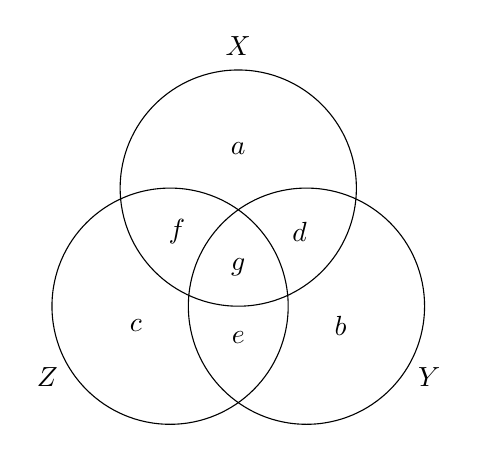
\begin{tikzpicture}
    % circles
    \draw (90:1) circle (1.5);
    \draw (210:1) circle (1.5);
    \draw (330:1) circle (1.5);

    % labels
    \node at (90:2.8) {$X$};
    \node at (330:2.8) {$Y$};
    \node at (210:2.8) {$Z$};
    
    \node at (90:1.5) {$a$};
    \node at (330:1.5) {$b$};
    \node at (210:1.5) {$c$};
    \node at (30:.9) {$d$};
    \node at (270:.9) {$e$};
    \node at (150:.9) {$f$};
    \node at (0:0) {$g$};
  \end{tikzpicture}
  \caption{Partition of $X \cup Y \cup Z$.  The quantities $a,b,c,d,e,f,g$
    represent the cardinalities of each disjoint set as shown.}
  \label{fig:partition}
\end{figure}

A related dissimilarity is the normalised symmetric difference,
$\delta_{\symdif} \colon 2^{\dset} \times 2^{\dset} \to \mathbb{R}^{\geq 0}$,
defined as:
\begin{equation*}
  \delta_{\symdif_n}(X,Y) =
  \begin{cases}
    \displaystyle \frac{|X \symdif Y|}{|X \cup Y|} & \text{if $X \cup Y \neq
      \emptyset$}, \\
    0 & \text{otherwise,}
  \end{cases}
\end{equation*}
for all $X,Y \in 2^{\dset}$.

\begin{thm}
  The normalised symmetric difference is a metric on $2^{\dset}$.
\end{thm}

The following proof was presented in \citep{yianilos91}, with some errors.  We
reproduce the proof here with the errors corrected.

\begin{proof}
  It is easy to see the function is nonnegative, symmetric and that
  $\delta_{\symdif_n}(X,Y)=0$ if and only if $X=Y$ for all $X,Y \in 2^{\dset}$
  so we will show that the triangle inequality holds which is:
  \begin{equation*}
    \frac{|X \symdif Y|}{|X \cup Y|} + \frac{|Y \symdif Z|}{|Y \cup Z|} \geq
    \frac{|X \symdif Z|}{|X \cup Y|}
  \end{equation*}
  or, equivalently:
  \begin{equation}
    \label{eq:tri-inequality}
    1 - \frac{|X \cap Y|}{|X \cup Y|} +
    1 - \frac{|Y \cap Z|}{|Y \cup Z|} \geq
    1 - \frac{|X \cap Z|}{|X \cup Z|}.
  \end{equation}

  We partition $X \cup Y \cup Z$ into disjoint subsets as shown in
  Figure~\ref{fig:partition} and let
  \begin{align*}
    a = |X \setminus (Y \cup Z)|,&\qquad
    b = |Y \setminus (X \cup Z)|,\\
    c = |Z \setminus (X \cup Y)|,&\qquad
    d = |(X \cap Y) \setminus Z|.\\
    e = |(Y \cap Z) \setminus X|.&\qquad
    f = |(Z \cap X) \setminus Y|.\\
    g = |X& \cap Y \cap Z|,
  \end{align*}
  and for convenience we let
  \begin{equation*}
    \xi  = |X \cup Y \cup Z|.
  \end{equation*}

  We can now write equation~(\ref{eq:tri-inequality}) as
  \begin{equation*}
    1 - \frac{d+g}{\xi -c} + 1 - \frac{e+g}{\xi -a} \geq 1 - \frac{f+g}{\xi -b}
  \end{equation*}
  which can be rewritten as
  \begin{equation*}
    \frac{d+g}{\xi -c} + \frac{e+g}{\xi -a} \leq \frac{f+g}{\xi -b} + 1.
  \end{equation*}

  Removing $b$ from the denominators on the LHS can only make the LHS
  greater, so it is sufficient to show that
  \begin{equation*}
    \frac{d+g}{\xi -b-c} + \frac{e+g}{\xi -a-b} \leq \frac{f+g}{\xi -b} + 1.
  \end{equation*}

  Now if we replace $1$ with $\frac{\xi -a-b-c}{\xi -a-b-c}$ on the RHS and add
  the fractions on the LHS we get
  \begin{multline*}
    \frac{(\xi -a-b)(d+g)+(\xi -b-c)(e+g)}{(\xi -b-c)(\xi -a-b)}\\
    \leq \frac{(\xi -a-b-c)(\xi -b)+(\xi -a-b-c)(f+g)}{(\xi -b)(\xi -a-b-c)}
  \end{multline*}
  which when we expand the denominators becomes
  \begin{multline*}
    \frac{(\xi -a-b)(d+g)+(\xi -b-c)(e+g)}{\xi ^2-\xi a-2\xi b-\xi c+ab+bc+b^2+ac}\\
    \leq \frac{(\xi -a-b-c)(\xi -b)+(\xi -a-b-c)(f+g)}{\xi ^2-\xi a-2\xi b-\xi c+ab+bc+b^2}.
  \end{multline*}
  Notice that the denominator on the LHS is equal to the denominator on the
  RHS with the addition of $ac$ so it cannot be less.  It is therefore
  sufficient to show that
  \begin{multline*}
    (\xi -a-b)(d+g)+(\xi -b-c)(e+g)\\
    \leq (\xi -a-b-c)(\xi -b)+(\xi -a-b-c)(f+g).
  \end{multline*}

  Starting with the LHS we have
  \begin{align*}
    &(\xi -a-b)(d+g)+(\xi -c-b)(e+g)\\
    &= (\xi -a-b-c)(d+g)+c(d+g)+(\xi -a-b-c)(e+g)+a(e+g)\\
    &\leq (\xi -a-b-c)(d+g)+c(\xi -a-b-c)\\
    &\qquad\qquad+(\xi -a-b-c)(e+g)+a(\xi -a-b-c)\\
    &= c(\xi -a-b-c)+(\xi -a-b-c)(d+e+g)\\
    &\qquad\qquad+g(\xi -a-b-c)+a(\xi -a-b-c)\\
    &\leq c(\xi -a-b-c)+(\xi -a-b-c)^2+g(\xi -a-b-c)+a(\xi -a-b-c)\\
    &= (\xi -a-b-c)(\xi -b)+g(\xi -a-b-c)\\
    &\leq (\xi -a-b-c)(\xi -b) + (f+g)(\xi -a-b-c).
  \end{align*}
\end{proof}

\subsubsection{Hausdorff distance}
\label{sec:hausdorff-distance}

\begin{figure}
  \centering
  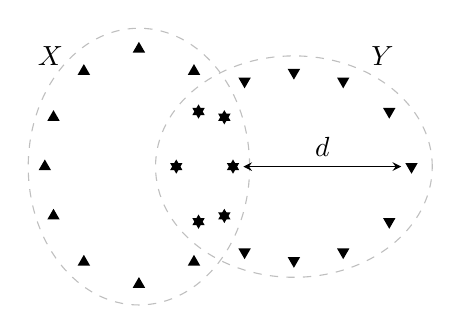
\begin{tikzpicture}[
    ]

    \draw [dashed,faint] (-2.8em,0) ellipse (4em and 5em);
    \draw [dashed,faint] (2.8em,0) ellipse (5em and 4em);

    % set 1 primary markers
    \begin{scope}[xshift=-2.8em,scale=0.85]
      \foreach \theta in {0,30,...,330} {
        \pgfmathparse{(4*5)/sqrt((5*cos(\theta))^2+(4*sin(\theta))^2)}
        \node [setnode1] (1set\theta) at (\theta:\pgfmathresult em) {};
      }
    \end{scope}
    % set 2 markers
    \begin{scope}[xshift=-2.8em,scale=0.85]
      \foreach \theta in {0,30,330} {
        \pgfmathparse{(4*5)/sqrt((5*cos(\theta))^2+(4*sin(\theta))^2)}
        \node [setnode2] at (\theta:\pgfmathresult em) {};
      }
    \end{scope}

    % set 2 primary markers
    \begin{scope}[xshift=2.8em,scale=0.85]
      \foreach \theta in {0,30,...,330} {
        \pgfmathparse{(5*4)/sqrt((4*cos(\theta))^2+(5*sin(\theta))^2)}
        \node [setnode2] (2set\theta) at (\theta:\pgfmathresult em) {};
      }
    \end{scope}
    % set 1 markers
    \begin{scope}[xshift=2.8em,scale=0.85]
      \foreach \theta in {150,180,210} {
        \pgfmathparse{(5*4)/sqrt((4*cos(\theta))^2+(5*sin(\theta))^2)}
        \node [setnode1] at (\theta:\pgfmathresult em) {};
      }
    \end{scope}

    \draw [symdist] (2set0) -- node[auto,swap] {$d$} (1set0);

    % labels
    \node at (-6em,4em) {$X$};
    \node at (6em,4em) {$Y$};
  \end{tikzpicture}
  \caption{$X$ and $Y$ are sets with elements labelled by \tikzuptriangle ~and
    \tikzupdtriangle ~respectively.  Elements in both sets are labelled with
    \tikzbotriangle .  The Hausdorff distance between $X$ and $Y$ is,
    informally, the greatest distance one must travel if starting from a point
    in one set and travelling to the closest point in the other.  This
    distance is marked by $d$ in the diagram.}
  \label{fig:haussdorf}
\end{figure}

Let $(M,d)$ be a metric space and $\mathcal{M}=2^M \setminus \{\emptyset\}$.
The Hausdorff distance, $\delta_{H} \colon \mathcal{M} \times \mathcal{M} \to
\mathbb{R}^{\geq 0}$, is defined as:
\begin{equation*}
  \delta_{H}(X,Y) = \max\left(\max_{x \in X} \min_{y \in Y} d(x,y),
                             \max_{y \in Y} \min_{x \in X} d(x,y)\right), 
\end{equation*}
for all $X,Y \in \mathcal{M}$.  The Hausdorff distance is a metric on
$\mathcal{M}$ \citep{braun2003geometry}.  This distance is illustrated in
Figure~\ref{fig:haussdorf} by showing the Hausdorff distance between two sets
with elements in a metric space.  In Chapter~\ref{cha:sum-squar-clust} we
present a new metric on $\mathcal{M}$.

\subsubsection{Linkage functions}
\label{sec:linkage-functions}

We conclude by remarking that the linkage functions, which are used in
hierarchical clustering, the topic of Section~\ref{sec:hier-clust-meth}, are
not generally metrics.  For a metric space, $(M,d)$, and $\mathcal{M}=2^M
\setminus \emptyset$, the \textit{single-linkage distance}, $\delta_{SL}
\colon \mathcal{M} \times \mathcal{M} \to \mathbb{R}^{\geq 0}$ is defined as:
\begin{equation*}
  \delta_{SL}(X,Y) = \min_{x \in X, y \in Y} d(x,y),
\end{equation*}
for all $X,Y \in \mathcal{M}$.  While single-linkage is a simple and intuitive
distance between sets, it is not a metric since distinct sets can have a
distance of zero.  The \textit{complete-linkage} and \textit{average-linkage}
dissimilarities are, in fact, not even distances.  These measures will be
discussed further in Section~\ref{sec:hier-clust-meth}.

% \subsection{Multiset datasets}
% \label{sec:multiset-datasets}

% It is tempting to think of a dataset and a metric defined on its elements as a
% metric space, but this is not necessarily correct.  The reason is that,
% contrary to the name, a dataset is not usually a set but a multiset.  Consider
% a dataset consisting of only the heights of some population of humans.
% Depending on the precision of the measurements taken, it would generally be
% expected that multiple subjects share the same height.  In order to have these
% observations in a set, some unique integer---an experiment number, say---would
% need to be attached to each observation.  But then the metric condition that
% $d(x,y)=0$ only if $x=y$ would be violated---in fact we would have only a
% \textit{pseudometric}.  We can get a proper metric if we define an equivalence
% relation $x \sim y$ if $d(x,y)=0$.  Then $(\dset/\sim,d)$ is a metric space.

% Most of the time we do not need to worry about this.  From now on a dataset,
% $\dset$, will implicitly mean $\dset/\sim$ as defined above unless stated
% otherwise.  Occasionally. though, it will be useful or necessary to consider
% the multiset $(\dset,\mu_{\dset})$ where $\dset$ is the underlying set, and
% $\mu_{\dset} \colon \dset \to \mathbb{N}_1$---a map from $\dset$ to the
% (nonzero) natural numbers---is called the membership function and tells us how
% many times an element appears in the multiset.

% A further generalisation is then possible: we can relax the definition of the
% membership function to $\mu_{\dset} \colon \dset \to \mathbb{R}_1$---a map
% from $\dset$ to the positive real numbers.  The dataset is then a fuzzy
% multiset.  Such datasets have been used in document clustering applications,
% for example in \citep{miyamoto2003information}, where objects can appear
% multiple times with a certain probability attached.  If the membership
% function if $\mu_{\dset} \colon \dset \to \mathbb{R}_1 \cap [0,1]$ then
% $(\dset,\mu_{\dset})$ is called a fuzzy set
% \citep{zadeh1965fuzzy,gottwald2010fuzzy}.

\section{Partitions}
\label{sec:partitions}

In this section we look at the properties of partitions of sets, how we can
compare partitions and how we can find partitions.  Throughout, we assume that
$n > 0$ and refer to a set of $n$ elements as an \textit{$n$-set}.

\subsection{The space of partitions}
\label{sec:space-partitions}

Given an $n$-set $\dset$, a $k$-partition $\clus = \{C_1,C_2,\dotsc,C_k\}$ of
$\dset$ is a set of $k \in \{1,\dotsc,n\}$ nonempty, pairwise-disjoint subsets
of $\dset$ such that $C_1 \cup C_2 \cup \dotsb \cup C_k = \dset$.  Following
common practice, we will refer to the elements of $\clus$ as
\textit{clusters}.

\begin{figure}
  \centering
  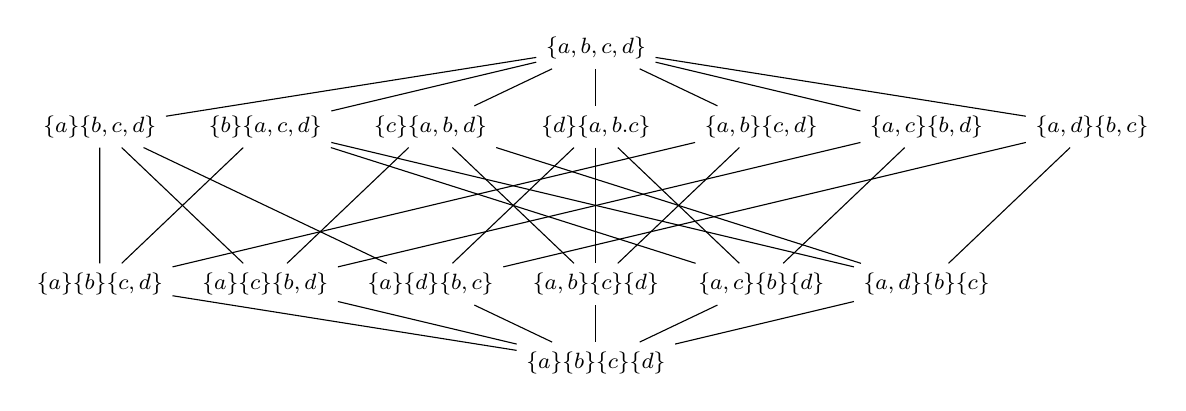
\begin{tikzpicture}[
    xscale=2.1, font=\footnotesize]

    % vertices
    
    \node (0) at (0,0) {$\{a,b,c,d\}$};

    \node (10) at (-3,-1) {$\{a\}\{b,c,d\}$};
    \node (11) at (-2,-1) {$\{b\}\{a,c,d\}$};
    \node (12) at (-1,-1) {$\{c\}\{a,b,d\}$};
    \node (13) at (0,-1) {$\{d\}\{a,b.c\}$};
    \node (14) at (1,-1) {$\{a,b\}\{c,d\}$};
    \node (15) at (2,-1) {$\{a,c\}\{b,d\}$};
    \node (16) at (3,-1) {$\{a,d\}\{b,c\}$};

    \node (20) at (-3,-3) {$\{a\}\{b\}\{c,d\}$};
    \node (21) at (-2,-3) {$\{a\}\{c\}\{b,d\}$};
    \node (22) at (-1,-3) {$\{a\}\{d\}\{b,c\}$};
    \node (23) at (0,-3) {$\{a,b\}\{c\}\{d\}$};
    \node (24) at (1,-3) {$\{a,c\}\{b\}\{d\}$};
    \node (25) at (2,-3) {$\{a,d\}\{b\}\{c\}$};

    \node (3) at (0,-4) {$\{a\}\{b\}\{c\}\{d\}$};

    % edges

    \draw (0) to (10);
    \draw (0) to (11);
    \draw (0) to (12);
    \draw (0) to (13);
    \draw (0) to (14);
    \draw (0) to (15);
    \draw (0) to (16);

    \draw (10) to (20);
    \draw (10) to (21);
    \draw (10) to (22);
    \draw (11) to (20);
    \draw (11) to (24);
    \draw (11) to (25);
    \draw (12) to (21);
    \draw (12) to (23);
    \draw (12) to (25);
    \draw (13) to (22);
    \draw (13) to (23);
    \draw (13) to (24);
    \draw (14) to (20);
    \draw (14) to (23);
    \draw (15) to (21);
    \draw (15) to (24);
    \draw (16) to (22);
    \draw (16) to (25);

    \draw (20) to (3);
    \draw (21) to (3);
    \draw (22) to (3);
    \draw (23) to (3);
    \draw (24) to (3);
    \draw (25) to (3);
  \end{tikzpicture}
  \caption{The Hasse diagram of the lattice of partitions of a set,
    $\dset=\{a,b,c,d\}$ \citep{meila-2005}.  Each vertex in the graph is a
    partition $\{C_1,\dotsc,C_k\}$ of $\dset$ which we denote by
    $C_1,\dotsc,C_k$ for clarity.}
  \label{fig:lattice}
\end{figure}

Let $\parts_{\dset}$ be the set of all partitions of $\dset$ and $\clus,\clus'
\in \parts_{\dset}$.  The partition $\clus$ is called a \textit{refinement} of
$\clus'$ if every element of $\clus$ is a subset of some element of $\clus'$.
We can then say that $\clus$ is \textit{finer-than-or-equal-to} $\clus'$,
which we notate $\clus \leq \clus'$ (or that $\clus'$ is
\textit{coarser-than-or-equal-to} $\clus$).  The relation $\leq$ imposes a
partial order on the elements of $\parts_{\dset}$.

The partially-ordered set $(\parts_{\dset},\leq)$ is called the
\textit{lattice of partitions} and can be represented in terms of a graph
called the \textit{Hasse diagram} associated with $\parts_{\dset}$.  The
vertex set of that graph is $\parts_{\dset}$ and its arc set consists of the
pairs $(\clus_1,\clus_2) \in \parts_{\dset} \times \parts_{\dset}$ such that
$\clus_2 < \clus_1$ and there exists no $\clus_3 \in \parts_{\dset}$ such that
$\clus_2 < \clus_3 < \clus_1$.  Informally, this means that $\clus_2$ can be
obtained by bisecting one cluster of $\clus_1$.

The Hasse diagram of the set $\dset = \{a,b,c,d\}$ is presented in
Figure~\ref{fig:lattice}.  The partition at the top is the coarsest partition
(a 1-partition) and the partition at the bottom is the finest partition (an
$n$-partition).

As this example suggests, a set can potentially support a very large number of
partitions.  For an $n$-set $\dset$ the cardinality of $\parts_{\dset}$ is
given by the \textit{Bell number} $B_n$
\citep{bell1934exponential,stanley2000enumerative} where $B_0=1$ and
\begin{equation*}
  B_n = \sum_{l=0}^{n-1} B_l \binom{n-1}{l} \qquad \text{for $n \geq 1$}.
\end{equation*}
Alternatively, $B_n$ is given by Dobi\'{n}ski's formula
\citep{dobinski1877summation}:
\begin{equation*}
  B_n = \frac{1}{e} \sum_{l=0}^{\infty} \frac{l^n}{l!} \qquad \text{for $n
    \geq 0$}.
\end{equation*}
We illustrate the growth of the Bell number in Table~\ref{tab:bell-number}.

\begin{table}
  \centering
  \begin{tabular}{rr}
    \toprule
    $n$ & $B_n$ \\
    \midrule
    5 & 52 \\
    10 & 115,975 \\
    15 & 1,382,958,545 \\
    20 & $5.17 \times 10^{13}$ \\
    25 & $4.64 \times 10^{18}$ \\
    \bottomrule
  \end{tabular}
  \caption{The value of the Bell number, $B_n$, for some selected values of
    $n$.  The value of $B_n$ is equivalent to the number of possible
    partitions of an $n$ element set.}
  \label{tab:bell-number}
\end{table}

\subsubsection{Fuzzy partitions}
\label{sec:fuzzy-partitions}

Partitions can be generalised to fuzzy partitions by letting the clusters be
fuzzy sets.  Fuzzy sets are collections of objects where each member of a
collection has a grade of membership associated to it \citep{zadeh1965fuzzy}.
Sets are a special case where the grades of membership are binary---objects
are either members of a set or they are not.  Fuzzy sets and partitions have
many applications including classification of data in the natural sciences
where membership is not precisely defined.

Formally, a fuzzy set is an ordered pair $(C,\mu_{C})$ consisting of an
underlying set $C$ and a membership function $\mu_{C} \colon C \to [0,1]$.
For some fuzzy set $(C,\mu_C)$ and element $x \in C$ $\mu_C(x) = 1$ means $x$
is a full member, $\mu_C(x) = 0$ means $x$ is not a member and $0 < \mu_C(x) <
1$ means $x$ is a fuzzy member.  If $\mu_C(x) = 0$ or $1$ for all $x \in C$
then the object is called by contrast a \textit{crisp set} and may be handled
by ordinary set theory \cite{zadeh1965fuzzy,klir1995fuzzy}.

A \textit{$k$-fuzzy-partition} of an $n$-set $\dset$ is a set of $k \in
\{1,\dotsc,n\}$ fuzzy sets: \[\{(C_1,\mu_1),(C_2,\mu_2),\dotsc,(C_k,\mu_k)\}\]
where $C_1 \cup \dotsb \cup C_k = \dset$, $C_i \neq \emptyset$ for all $i \in
\{1,\dotsc,k\}$ and $\sum_{i=1}^{k} \mu_i(x) = 1$ for all $x \in \dset$.  Note
that the underlying sets of the fuzzy sets $(C_i,\mu_i)$ are not necessarily
pairwise disjoint, so elements can belong to more than one cluster.

\subsection{Comparing partitions}
\label{sec:comparing-partitions}

An attractive way to find partitions of a set is by means of a partitional
clustering method.  Many methods exist---we will review some in
Section~\ref{sec:part-clust-algor}---and, depending on their respective
approach to the problem, they all tend to produce different partitions.  To
further complicate matters, some methods are nondeterministic so can
potentially produce different partitions each time they are used.

For the purposes of comparing and assessing clustering methods it is therefore
useful to be able to compare partitions.  Many measures have been devised for
this purpose, including similarity measures and dissimilarity measures, of
which some are metrics.  Existing methods fall into four main categories; for
two partitions $\clus_1$ and $\clus_2$ of a set $\dset$, these are:
\begin{description}
\item[Pair counting] which measures the agreement and disagreement between
  $\clus_1$ and $\clus_2$ by means of counting pairs of element in $\dset$,
\item[Set matching] which ``matches'' clusters in $\clus_1$ with clusters in
  $\clus_2$ and measures the similarity between matched sets,
\item[Information theoretic] which uses information theory to measure the
  information and mutual information contained in $\clus_1$ and $\clus_2$,
\item[Density profile] which takes into account the values of the data when
  computing the measure.
\end{description}

We will review measures belonging to the first three categories in this
section.  The fourth category consists of a single measure called ADCO which
we will analyse in Chapter~\ref{cha:sum-squar-clust}.

To be able to describe the measures in detail, we need to introduce some more
terminology.  Let $\dset = \{x_1,x_2,\dotsc,x_n\}$ be an $n$-set with $n \geq
2$ and again, as before, let $\clus_1 = \{C_{11},C_{12},\dotsc,C_{1k}\}$ and
$\clus_2 = \{C_{21},C_{22},\dotsc,C_{2k'}\}$ be two partitions of $\dset$ with
$k$ and $k'$ clusters, respectively.  We denote, for some $x \in \dset$, and a
partition, $\clus$, of $\dset$, the cluster in $\clus$ that contains $x$ by
$\clus(x)$.  The \textit{confusion matrix} associated with $\clus_1$ and
$\clus_2$ is the $k \times k'$ matrix $[n_{ij}]$ where $n_{ij} = |C_{1i} \cap
C_{2j}|$.  It is used for the calculation of both pair counting and set
matching measures.

To illustrate these definitions and the comparison measures we review below,
we will use two example partitions $\clus^*_1$ and $\clus^*_2$ of the set
$\dset^* = \{1,\dotsc,9\}$ throughout this section:
\begin{equation}
  \label{eq:example-parts}
  \clus^*_1 = \{C^*_{11},C^*_{12},C^*_{13}\},\qquad
  \clus^*_2 = \{C^*_{21},C^*_{22},C^*_{23},C^*_{24}\}
\end{equation}
where
\begin{align*}
  C^*_{11}&=\{1,2,3\},\quad C^*_{12}=\{4,5,6\},\quad C^*_{13}\{7,8,9\} \quad \text{and}\\
  C^*_{21}&=\{1,4\},\quad C^*_{22}=\{2,3,6\},\quad C^*_{23}=\{5,8\},\quad C^*_{24}\{7,9\}.
\end{align*}
Then, for example, we have $\clus^*_1(3) = C^*_{11}$, and the confusion matrix
associated with $\clus^*_1$ and $\clus^*_2$ is:
\begin{equation*}
  [n_{ij}]^*=\left[
  \begin{matrix}
    1 & 2 & 0 & 0 \\
    1 & 1 & 1 & 0 \\
    0 & 0 & 1 & 2
  \end{matrix}
  \right]
\end{equation*}

\subsubsection{Pair counting}
\label{sec:pair-counting}

There are $\binom{n}{2}$ distinct pairs of elements in $\dset$.  For each
distinct pair $(a,b) \in \dset \times \dset$ one of the following is true:
\begin{align*}
\clus_1(a)=\clus_1(b) &\text{ and } \clus_2(a)=\clus_2(b),\\
\clus_1(a)\neq \clus_1(b) &\text{ and } \clus_2(a)\neq \clus_2(b),\\
\clus_1(a)=\clus_1(b) &\text{ and } \clus_2(a)\neq \clus_2(b),\\
\clus_1(a)\neq \clus_1(b) &\text{ and } \clus_2(a)=\clus_2(b).
\end{align*}
Counting the number of element in each category gives us four counts which are
defined formally as:
\begin{align*}
  N_{11} &= |\{(a,b) \in \dset \times \dset \colon
              \clus_1(a)=\clus_1(b) \text{ and } \clus_2(a)=\clus_2(b)
            \}|, \\
  N_{00} &= |\{(a,b) \in \dset \times \dset \colon
              \clus_1(a)\neq\clus_1(b) \text{ and } \clus_2(a)\neq\clus_2(b)
            \}|, \\
  N_{10} &= |\{(a,b) \in \dset \times \dset \colon
              \clus_1(a)=\clus_1(b) \text{ and } \clus_2(a)\neq\clus_2(b)
            \}|, \\
  N_{01} &= |\{(a,b) \in \dset \times \dset \colon
              \clus_1(a)\neq\clus_1(b) \text{ and } \clus_2(a)=\clus_2(b)
            \}|.
\end{align*}
The size of $N_{11}$ and $N_{00}$ are considered to be measurements of
\textit{agreement} between $\clus_1$ and $\clus_2$, while $N_{10}$ and
$N_{01}$ are considered measurements of \textit{disagreement}.

The measures based on pair counting can all be expressed in terms of these
four counts.  Clearly \[N_{11}+N_{00}+N_{10}+N_{01} = \binom{n}{2}\] is always
satisfied.  The quantities $N_{11},N_{00},N_{10}$ and $N_{01}$ can all be
obtained from the confusion matrix using the following formul\ae
\citep{hubert-arabie-1985}:
\begin{align*}
  N_{11} &= \frac{1}{2} \sum_{i=1}^{k} \sum_{j=1}^{k'} n_{ij}(n_{ij}-1),\\
  N_{00} &= \frac{1}{2} \left(n^2 + \sum_{i=1}^{k} \sum_{j=1}^{k'} n_{ij}^2
                             - \sum_{i=1}^{k}
                                \left(\sum_{j=1}^{k'} n_{ij} \right)^2
                             - \sum_{j=1}^{k'}
                                \left(\sum_{i=1}^{k} n_{ij} \right)^2
                       \right),\\
  N_{10} &= \frac{1}{2} \left(\sum_{i=1}^{k}
                              \left(\sum_{j=1}^{k'} n_{ij} \right)^2
                             - \sum_{i=1}^{k} \sum_{j=1}^{k'} n_{ij}^2
                       \right),\\
  N_{01} &= \frac{1}{2} \left(\sum_{j=1}^{k'}
                              \left(\sum_{i=1}^{k} n_{ij} \right)^2
                             - \sum_{i=1}^{k} \sum_{j=1}^{k'} n_{ij}^2
                       \right).
\end{align*}
The four counts for our example partitions $\clus^*_1$ and $\clus^*_2$ are:
\begin{equation*}
  N_{11} = 2,\quad
  N_{00} = 23,\quad
  N_{10} = 7,\quad
  N_{01} = 4.
\end{equation*}

One of the simplest pair counting measures between $\clus_1$ and $\clus_2$ is
the widely-used \textit{Rand index} $\partcomparen{R}$ introduced in
\citep{rand-1971} and defined as:
\begin{equation*}
\partcompare{R} = \frac{(N_{11}+N_{00})}{\binom{n}{2}}.
\end{equation*}
The Rand index is a similarity measure with a lower bound of 0 and an upper
bound of 1.  \citet{hubert-arabie-1985} use the following variation:
\[\partcompare{HA} = (N_{11}+N_{00}-N_{10}-N_{01})/\binom{n}{2}.\]

\citet{wallace-1983} introduced two asymmetric measures for comparing
$\clus_1$ and $\clus_2$ defined as:
\begin{equation*}
  \mathcal{W}_{I}(\clus_1,\clus_2) =
  \frac{N_{11}}{\sum_{i=1}^{k} |C_{i1}|(|C_{1i}|-1)/2},
\end{equation*}
and
\begin{equation*}
  \mathcal{W}_{II}(\clus_1,\clus_2) =
  \frac{N_{11}}{\sum_{j=1}^{k'} |C_{2j}|(|C_{2j}|-1)/2}.
\end{equation*}
$\mathcal{W}_{I}$ and $\mathcal{W}_{II}$ represent the probabilities that, for
a pair of elements $(a,b) \in \dset \times \dset$ with
$\clus_1(a)=\clus_1(b)$, we also have $\clus_2(a)=\clus_2(b)$, and vice versa.
A symmetric similarity measure for $\clus_1$ and $\clus_2$ can be obtained by
taking the geometric mean of the Wallace measures:
\begin{equation*}
  \partcompare{F} = \sqrt{\mathcal{W}_{I}(\clus_1,\clus_2)
                          \mathcal{W}_{II}(\clus_1,\clus_2)}.
\end{equation*}
This measure was also introduced independently by Fowlkes and Mallows in
\citep{fowlkes-mallows-1983}.

The \textit{Jaccard coefficient} $\partcomparen{J}$ is another widely-used
similarity measure and is defined, for $\clus_1$ and $\clus_2$, as:
\begin{equation*}
  \partcompare{J} = \frac{N_{11}}{N_{10}+N_{01}+N_{11}}.
\end{equation*}

It should be noted that all measures reviewed so far are similarity measures.
The \textit{Mirkin metric} $\partcomparen{M}$ for measuring dissimilarity
between $\clus_1$ and $\clus_2$ was originally introduced in
\citep{mirkin1996mathematical} and is defined as
\begin{equation*}
  \partcompare{M} = \sum_{i=1}^{k} |C_{1i}|^2 +
                    \sum_{j=1}^{k'} |C_{1j}|^2 +
                    2\sum_{i=1}^{k}\sum_{j=1}^{k'} n_{ij}^2,
\end{equation*}
where $[n_{ij}]$ again denotes the confusion matrix associated with $\clus_1$
and $\clus_2$.  As it turns out, \[\partcompare{M}=2(N_{10}+N_{01}).\] The
closely related measure: \[\partcompare{AB}=(N_{10}+N_{01})/\binom{n}{2}\] is
also a metric on $\parts_{\dset}$ and was used by
\citet{mirkin1970measurement} and \citet{arabie1973multidimensional}.

\begin{table}
  \centering
  \begin{tabular}{lr}
    \toprule
    Name & Measure \\
    \midrule
    Rand index          & $\partcomparest{R} \approx 0.694$ \\
    Wallace measures    & $\mathcal{W}_{I}(\clus^*_1,\clus^*_2) \approx 0.222$ \\
                        & $\mathcal{W}_{II}(\clus^*_1,\clus^*_2) \approx 0.333$ \\
    Fowlkes \& Mallows  & $\partcomparest{F} \approx 0.272$ \\
    Jaccard coefficient & $\partcomparest{J} \approx 0.154$ \\
    Merkin metric       & $\partcomparest{M} = 22.00$ \\
    \bottomrule
  \end{tabular}
  \caption{Various pair counting based measures applied to the example
    partitions $\clus^*_1$ and $\clus^*_2$~\eqref{eq:example-parts}.}
  \label{tab:pair-counting-comparison}
\end{table}

The values of the reviewed pair counting measures when applied to $\clus^*_1$
and $\clus^*_2$ are given in Table~\ref{tab:pair-counting-comparison}.

\subsubsection{Set matching}
\label{sec:set-matching}

Set matching measures for partitions $\clus_1$ and $\clus_2$ are based on
comparisons between matched pairs of clusters.  Each pair to be compared
consists of one element of $\clus_1$ and one of $\clus_2$.  All of the
measures that we review here are based on the confusion matrix, meaning that
they use the cardinality of the intersection between two clusters as a
similarity measure.  The differences between the measures are essentially due
to the way that they find the matched pairs of clusters for comparison.

As before, let $\dset$ be an $n$-set and let $\clus_1 =
\{C_{11},\dotsc,C_{1k}\}$ and $\clus_2 = \{C_{21},\dotsc,C_{1k'}\}$, where
$k,k' \geq 1$, denote two partitions of $\dset$.  Also assume, without loss of
generality, that $k' \geq k$.  Then, a \textit{matching} between $\clus_1$ and
$\clus_2$ is a function $\sigma \colon \{1,\dotsc,k\} \to \{1,\dotsc,k'\}$.

\begin{figure}
  \centering
  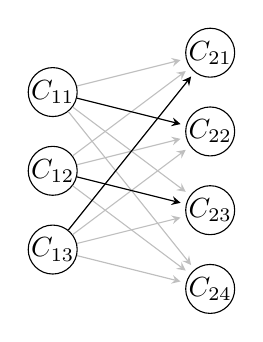
\begin{tikzpicture}[
    % >=stealth,
    % clus/.style={circle,draw=black,inner sep=0,minimum size=5mm},
    % dist/.style={->,shorten >=2pt},
    % faint/.style={dist,gray!50},
    nonmatch/.style={dist,faint},
    match/.style={dist,black}
    ]

    \node [clus] (c11) at (0,1) {$C_{11}$};
    \node [clus] (c12) at (0,0) {$C_{12}$};
    \node [clus] (c13) at (0,-1) {$C_{13}$};

    \node [clus] (c21) at (2,1.5) {$C_{21}$};
    \node [clus] (c22) at (2,.5) {$C_{22}$};
    \node [clus] (c23) at (2,-.5) {$C_{23}$};
    \node [clus] (c24) at (2,-1.5) {$C_{24}$};

    % join them all
    \foreach \x in {1,2,3} {
      \foreach \y in {1,2,3,4} {
        \draw [nonmatch] (c1\x) to (c2\y);
      }
    }

    % matches
    \draw [match] (c11) to (c22);
    \draw [match] (c12) to (c23);
    \draw [match] (c13) to (c21);
  \end{tikzpicture}
  \caption{The clusters belonging to two partitions $\{C_{11},\dotsc,C_{13}\}$
    and $\{C_{21},\dotsc,C_{24}\}$ are shown with all similarities between
    pairs shown in grey.  The black lines represent one possible matching
    between the clusters.  In this case, the matching is an injection.}
  \label{fig:matching}
\end{figure}

\citet{meila-2001} introduced a set matching measure for measuring the
similarity between $\clus_1$ and $\clus_2$.  It finds a matching $\sigma$
using the following heuristic: let $[n_{ij}]$ be the $k \times k'$ confusion
matrix associated with $\clus_1$ and $\clus_2$.  Compute $n_{ab} = \argmax
\{n_{ij} \colon 1 \leq i \leq k, 1 \leq j \leq k'\}$ and put $\sigma(a) \gets
b$.  Repeat the process for the $(k-1) \times (k'-1)$ submatrix obtained by
deleting row $a$ and column $b$, and so on until $k$ matches have been made.
This process clearly finds an injection for $\sigma$ and then the similarity
of $\clus_1$ and $\clus_2$ based on that matching is:
\begin{equation*}
  \partcompare{H} = \frac{1}{n} \sum_{i=1}^{k} n_{i \sigma(i)}.
\end{equation*}

A second similarity measure on $\parts_{\dset}$, denoted $\partcomparen{L}$
and introduced by \citet{larsen-aone-1999} simply computes a maximal match for
each cluster in $\clus_1$ and $\clus_2$:
\begin{equation*}
  \partcompare{L} = \frac{1}{k} \sum_{i=1}^{k} \max_{1 \leq j \leq k'}
                                             \frac{2n_{ij}}{|C_{1i}|+|C_{2j}|}.
\end{equation*}

A dissimilarity measure $\partcomparen{V}$, which is a metric on
$\parts_{\dset}$, was introduced by \citet{van-dongen-2000}.  This measure,
again, computes maximal matches for each cluster in $\clus_1$ and $\clus_2$:
\begin{equation*}
  \partcompare{V} = 2n - \sum_{i=1}^{k} \max_{1 \leq j \leq k'} n_{ij}
                         \sum_{j=1}^{k'} \max_{1 \leq i \leq k} n_{ij}.
\end{equation*}

A second metric on $\parts_{\dset}$ denoted by $\partcomparen{CE}$ is due to
\citet{meila-2005} and is known by the name \textit{classification error}.
Like $\partcomparen{H}$, this measure computes an injection for $\sigma$, but
instead of using a heuristic finds a globally optimal injection in the set
$S_k$ of all possible injections from $\{1,\dotsc,k\}$ to $\{1,\dotsc,k'\}$:
\begin{equation*}
  \partcompare{CE} = 1 - \frac{1}{n} \max_{\sigma \in S_k}
                                     \sum_{i=1}^{k} n_{i \sigma(i)}.
\end{equation*}
Note that the injection, $\sigma$, can be found in polynomial time.  Also,
\[\partcompare{CE} \leq 1\] for all partitions $\clus_1$ and $\clus_2$ of
$\dset$.  The values of the set matching measures when applied to our example
partitions $\clus^*_1$ and $\clus^*_2$ are given in
Table~\ref{tab:set-matching-comparison}.

\begin{table}
  \centering
  \begin{tabular}{lr}
    \toprule
    Name & Measure \\
    \midrule
    Meilă \& Heckerman   & $\partcomparest{H} \approx 0.556$ \\
    Larsen \& Aone       & $\partcomparest{L} \approx 0.622$ \\
    Van Dongen metric    & $\partcomparest{V} = 7.000$ \\
    Classification Error & $\partcomparest{CE} \approx 0.445$ \\
    
    \bottomrule
  \end{tabular}
  \caption{Various set matching based measures applied to the example
    partitions $\clus^*_1$ and $\clus^*_2$~\eqref{eq:example-parts}.}
  \label{tab:set-matching-comparison}
\end{table}

\citet{meila-2007} and \citet{bae2010comparison} point out that all of these
measures suffer from the so-called ``problem of matching'' which we will now
illustrate.  Given a partition $\clus=\{C_1,\dotsc,C_k\}$ with $k\geq 2$
equally sized clusters, we can obtain a partition $\clus'$ from $\clus$ by
moving a fraction $f$ of the objects from each cluster $C_{i}$ to $C_{i+1}$,
with the indices taken$\mod k$.  We can obtain a further partition $\clus''$
from $\clus$ by taking the same fraction from each cluster in $C \in \clus$
and distributing the objects evenly among all other clusters in $\clus
\setminus \{C\}$.  Our intuition would be that the similarity between $\clus$
and $\clus'$ is not the same as the similarity between $\clus$ and $\clus''$.
However,
\begin{align*}
  \partcomparep{H} = \partcomparepp{H},&\quad
  \partcomparep{L} = \partcomparepp{L},\\
  \partcomparep{V} = \partcomparepp{V},&\quad
  \partcomparep{CE} = \partcomparepp{CE}
\end{align*}
whenever $0< f < 1/2$.

To give a numerical example, let $\dset = \{1,\dotsc,15\}$,
\begin{equation*}
  \clus = \{\{1,2,3,4,5\},\{6,7,8,9,10\},\{11,12,13,14,15\}\}
\end{equation*}
be a partition of $\dset$ and $f = 2/5$.  Then
\begin{equation*}
\clus' = \{\{1,2,3,14,15\},\{6,7,8,4,5\},\{11,12,13,9,10\}\}
\end{equation*}
and
\begin{equation*}
\clus'' = \{\{1,2,3,9,14\},\{6,7,8,4,15\},\{11,12,13,5,10\}\}
\end{equation*}
are partitions of $\dset$ obtained from $\clus$ as described above.  In this
case we have
\begin{align*}
  \partcomparep{H} = \partcomparepp{H} = 3/5,&\quad
  \partcomparep{L} = \partcomparepp{L} = 3/5,\\
  \partcomparep{V} = \partcomparepp{V} = 12,&\quad
  \partcomparep{CE} = \partcomparepp{CE} = 2/5.
\end{align*}

\subsubsection{Information theoretic}
\label{sec:inform-theor}

Two measures which use information theory are \textit{Normalized Mutual
  Information} \citep{fred-jain-2003} and \textit{Variation of Information}
\citep{meila-2007}.  For the remainder of this section we will focus on the
latter and refer the reader to \citep{fred-jain-2003} for details on the
former.

Variation of Information is based on both how much information is contained in
each partition and how much information one partition contains about the other
(their mutual information).

Let $\clus = \{C_{1},\dotsc,C_{k}\}$, where $k \geq 1$, be partition of an
$n$-set $\dset$.  Then the \textit{information} contained in $\clus$ is
measured by:
\begin{equation}
  \label{eq:entropy}
  H(\clus) = -\sum_{i=1}^{k} P_{\clus}(i) \log_b P_{\clus}(i),
\end{equation}
where
\begin{equation*}
  P_{\clus}(i) = \frac{|C_{i}|}{k}, \qquad \text{for $i = 1,\dotsc,k$}.
\end{equation*}
Informally, $P_1(i)$, is the probability that an object picked randomly from
$\dset$ is in cluster $C_{1i}$.  This measure is sometimes called
\textit{entropy}.  The base of the logarithm determines the unit of
information; for example, the bases $b=2,b=e$ and $b=10$ give the information
in so-called \textit{bits}, \textit{nits} and \textit{Hartleys}, respectively
\citep[see][]{kullback68information}.

Now, with $\clus_1 = \{C_{11},\dotsc,C_{1k}\}$ and $\clus_2 =
\{C_{21},\dotsc,C_{1k'}\}$, where $k,k' \geq 1$, the mutual information,
$I(\clus_1,\clus_2)$, between $\clus_1$ and $\clus_2$ is given by:
\begin{equation}
  \label{eq:mutualinf}
  I(\clus_1,\clus_2) = \sum_{i=1}^{k} \sum_{i=1}^{k'}
  P_{12}(i,j) \log_b \frac{P_{12}(i,j)}{P_{\clus_1}(i)P_{\clus_2}(j)},
\end{equation}
where
\begin{equation*}
  P_{12}(i,j) = \frac{|C_{1i} \cap C_{2j}|}{n}, \qquad \text{for $i =
    1,\dotsc,k,j = 1,\dotsc,k'$}.
\end{equation*}
Informally, $P_{12}(i,j)$ is the probability that an object picked randomly
from $\dset$ is in both $C_{1i}$ and $C_{2j}$.

The \textit{Variation of Information}, $\partcomparen{VI}$, between $\clus_1$
and $\clus_2$ is then defined as:
\begin{equation*}
  \partcompare{VI} = H(\clus_1) + H(\clus_2) - 2I(\clus_1,\clus_2).
\end{equation*}

As it turns out, $\Delta_{\mathcal{VI}}$ is a metric on $\parts_{\dset}$ and
has some attractive properties.  These include that it is $n$-invariant,
meaning its value depends only on the relative sizes of the clusters in
$\clus_1$ and $\clus_2$ and not on the size of $n$.  Further, it is bounded
for all $n$ by
\begin{equation*}
  \partcompare{VI} \leq \log_b n.
\end{equation*}
Finally, if $\max(k,k') \leq k^*$ where $k^* \leq \sqrt{n}$ then
\begin{equation*}
  \partcompare{VI} \leq 2 \log_b k^*
\end{equation*}
holds.

\begin{table}
  \centering
  \begin{tabular}{lr}
    \toprule
    Name & Measure \\
    \midrule
    Information & $H(\clus^*_1) \approx 1.585$ \\
                & $H(\clus^*_2) \approx 1.975$ \\
    Mutual information & $I(\clus^*_1,\clus^*_2) \approx 0.834$ \\
    Variation of Information & $\partcomparest{VI} \approx 1.891$
    \\
    \bottomrule
  \end{tabular}
  \caption{Variation of Information and its components applied to the example
    partitions $\clus^*_1$ and $\clus^*_2$~\eqref{eq:example-parts} using base
    2 for the logarithms in equations~\eqref{eq:entropy} and
    \eqref{eq:mutualinf}.}
  \label{tab:vi-comparison}
\end{table}

The values of Variation of Information and its components applied to our
example partitions, $\clus^*_1$ and $\clus^*_2$, are given in
Table~\ref{tab:vi-comparison}.
\\\\
\noindent We conclude this section with mentioning a further measure called
ADCO, which is a density profile based measure.  We will save discussion of
this measure until we introduce our own Assignment Metric later since these
two metrics share a unique feature possessed by no other measure discussed in
this section.  Namely, they take into account that the partitions to be
compared are partitions of a dataset themselves, with elements that have a
metric defined on them.

\section{Partitional clustering}
\label{sec:part-clust-algor}

The problem of finding meaningful partitions of a dataset is called
\textit{partitional clustering}.  Broadly speaking, the applications of
partitional clustering fall into two categories: \textit{data reduction} and
\textit{object classification}.

Data reduction may be necessary when a dataset is large and it is deemed that
only an essence of the data is wanted for a particular application.  For
example, if geographical data is to be displayed on a map then a large dataset
may not be desirable due to the visual clutter it would create.  Clustering
can be used to reduce the dataset into a more visually appealing and usable
subset.

Object classification is concerned with grouping data into a number of
classes.  For example, given a dataset obtained by market research one may
wish to find different classes of consumers in order to observe their habits
and predict future behaviour.  A further example is document clustering is an
important area concerned with clustering on datasets consisting of objects
written in a natural language.  Search engines such as those found on the
World Wide Web use document clustering to suggest, among other things,
``similar'' documents to the one a user is currently interested in
\citep{steinbach2000comparison}.

\subsection{Criteria}
\label{sec:criteria}

Informally, a meaningful partition of a dataset $(D,d)$ is one which contains
clusters that are homogeneous---meaning objects belonging to the same cluster
are similar---and well-separated---meaning objects belonging to different
clusters are dissimilar, according to $d$.

The task of judging a particular partition of a dataset based on these
informal standards is often a highly subjective one but, nevertheless, many
objective criteria have been devised for the purposes of automatic clustering.
The aim of a partitional clustering algorithm is to find a globally optimal
solution, that is a partition which has maximum homogeneity or separation or
both, according to a particular criterion.

\subsubsection{Dissimilarity based criteria}
\label{sec:diss-based-crit}

The most general criteria for homogeneity and separation are defined only
using dissimilarities.  To make this more precise, let $\dset$ be an $n$-set
with $n\geq 1$, $d \colon \dset \times \dset \to \mathbb{R}^{\geq 0}$ be a
dissimilarity on $\dset$ and $C \subseteq \dset$ be some cluster.
\\\\
\noindent Criteria that measure the homogeneity of $C$ include the
\textit{diameter} of $C$, which is defined as the maximum dissimilarity
between two members of $C$:
\begin{equation*}
  \max_{x,y \in C} d(x,y),
\end{equation*}
the \textit{radius} of $C$, which is defined as the minimum of the maximum
dissimilarities between each member and another member of $C$:
\begin{equation*}
  \min_{x \in C_i} \max_{y \in C} d(x,y)
\end{equation*}
the \textit{star} of $C$, which is defined as the minimum of the sums of
dissimilarities between each member and every other member of $C$:
\begin{equation*}
  \min_{c \in C} \sum_{x \in C} d(x,c),
\end{equation*}
and the \textit{clique} of $C$, which is defined as the sum of dissimilarities
between each pair of members of $C$:
\begin{equation*}
  \sum_{x,y \in C} d(x,y).
\end{equation*}

Criteria that measure the separation of $C$ from every other cluster include
the \textit{split} of $C$, which is defined as the minimum dissimilarity
between a member of $C$ and an element in $\dset \setminus C$:
\begin{equation*}
  \min_{x \in C, y \in \dset \setminus C} d(x,y),
\end{equation*}
and the \textit{cut} of $C$, which is defined as the sum of dissimilarities
between all members of $C$ and all elements in $\dset \setminus C$:
\begin{equation*}
  \sum_{x \in C} \sum_{y \in \dset \setminus C} d(x,y).
\end{equation*}

Dissimilarity based criteria for partitions can then be obtained from the
above measures for clusters by simply taking the sum over all clusters in a
partition.  We call these criteria \textit{sum-of-diameters},
\textit{sum-of-radii}, \textit{sum-of-stars} and so on.  Alternatively one
could simply take the maximum or minimum value, as appropriate, over the
clusters which we would call \textit{max-diameter}, \textit{max-radius},
\textit{min-cut} and so on.  The aim of a clustering method is then to
minimise a criterion for homogeneity or maximise a criterion for separation.

Some criteria for homogeneity are equivalent to criteria for separation.  Most
notably, minimising sum-of-cliques is equivalent to maximising sum-of-cuts.
Such criteria are therefore criteria for both homogeneity and separation.

As it turns out, criteria which only measure one or the other, like min-split
and max-diameter, are often conflicting.  For example, maximising min-split
produces clusters with poor homogeneity, called the \textit{chaining effect},
and minimising max-diameter results in clusters with poor separation, called
the \textit{dissection effect}.  Such criteria are therefore not so useful on
their own, but one way to overcome this problem is to consider a
\textit{bicriterion}, that is simultaneously consider a criterion for
homogeneity and a criterion for separation \citep{delattre1980bicriterion}.

\subsubsection{Scatter matrix based criteria}
\label{sec:scatter-matrix-based}

If the dataset of interest is embedded in $m$-dimensional Euclidean space,
with $m \geq 1$, then the following criteria based on the scatter or
dispersion matrix of \citet{wilks60} are possible.  To make this more precise,
let $d_E$ denote the Euclidean distance on $\dset$ and denote a vector
$\vec{v} \in \mathbb{R}^m$ by $\vec{v} = (v_1,\dotsc,v_m)$.  Suppose $C =
\{\vec{x}_1,\dotsc,\vec{x}_n\} \subset \mathbb{R}^m$, then the \textit{total
  scatter matrix} of $C$, $\mathbf{T}_{C}$, is the $m \times m$ matrix defined
as:
\begin{equation*}
  \mathbf{T}_{C} = \sum_{i=1}^{n} (\vec{x}_i - \vec{c})(\vec{x}_i - \vec{c})^{\mathrm{T}}
\end{equation*}
where $\vec{c}$ is the mean value of $\dset$.

For $\clus = \{C_1,\dotsc,C_k\}$, a partition of an $n$-set $\dset =
\{\vec{x}_1,\dotsc,\vec{x}_n\}$, two further matrices are associated.  The
\textit{within-cluster scatter matrix}, $\mathbf{W}_{\clus}$, is defined as:
\begin{equation*}
\mathbf{W}_{\clus} = \sum_{i=1}^{k} \mathbf{T}_{C_i},
\end{equation*}
where $\mathbf{T}_{C_i}$ is the total scatter matrix for cluster $C_i$ of
$\clus$.  The \textit{between-cluster scatter matrix}, $\mathbf{B}_{\clus}$,
is defined as:
\begin{equation*}
  \mathbf{B}_{\clus} =
  \sum_{i=1}^{k} |C_i| (\vec{c}_i - \bar{\vec{x}}) (\vec{c}_i -
  \bar{\vec{x}})^{\mathrm{T}}
\end{equation*}
where $\vec{c}_i$ is the mean of cluster $C_i$ and $\bar{\vec{x}}$ is the mean
of $\dset$.  These matrices are related by the equality
\begin{equation*}
  \mathbf{T}_{\dset} = \mathbf{W}_{\clus} + \mathbf{B}_{\clus}.
\end{equation*}

A popular criterion used in clustering algorithms is the minimisation of the
trace of $\mathbf{W_{\clus}}$, denoted $\tr(\mathbf{W_{\clus}})$.  Since
\begin{equation*}
  \tr(\mathbf{T_{\dset}}) = \tr(\mathbf{W_{\clus}}) + \tr(\mathbf{B_{\clus}}),
\end{equation*}
and $\tr(\mathbf{T}_{\dset})$ is a constant, it follows that minimising
$\tr(\mathbf{W_{\clus}})$ is equivalent to maximising
$\tr(\mathbf{B_{\clus}})$.

Intriguingly, $\tr(\mathbf{W}_{\clus})$ is also equivalent to the sum over all
clusters $C \in \clus$ of the sum of Euclidean distances squared between each
element $\vec{x} \in C$ and the mean $\vec{c}$ of $C$:
\begin{equation}
  \label{eq:tr(W)}
  \tr(\mathbf{W_{\clus}}) = \sum_{i=1}^{k} \sum_{\vec{x} \in C_i}
  d_{E}^2(\vec{x},\vec{c}_i).
\end{equation}
This can be seen easily by examining the main diagonal of the total scatter
matrix for each cluster $C \in \clus$, as illustrated here:
\begin{multline*}
  \mathbf{T}_{C} = \\
  \sum_{\vec{x} \in C}
  \begin{bmatrix}
    (x_1-c_{1})^2 & (x_1-c_{1})(x_2-c_{2}) & \cdots &
    (x_1-c_{1})(x_m-c_{m}) \\
    (x_2-c_{2})(x_1-c_{1}) & (x_2-c_{2})^2 & \cdots &
    (x_2-c_{2})(x_m-c_{m}) \\
    \vdots & \vdots & \ddots & \vdots \\
    (x_m-c_{m})(x_1-c_{1}) & (x_m-c_{m})(x_2-c_{2}) & \cdots &
    (x_m-c_{m})^2
  \end{bmatrix}
\end{multline*}
where $\vec{c}=(c_1,\dotsc,c_m)$ is the mean of $C$.

Similarly, $\tr(\mathbf{B_{\clus}})$ is equivalent to the sum of Euclidean
distances squares between the mean $\vec{c}$ of a cluster $C$ and
$\bar{\vec{x}}$, the mean of $\dset$, multiplied by the size of $C$:
\begin{equation}
  \label{eq:tr(B)}
  \tr(\mathbf{B_{\clus}}) = \sum_{i=1}^{k} |C_i| d_E^2(\vec{c}_i,\bar{\vec{x}}).
\end{equation}

For this reason, the trace of $\mathbf{W}_{\clus}$ is often called
``sum-of-squares'', but this name is ambiguous since any criterion utilising
sums of distances squared could have this name.  We therefore call the
criterion shown in equation~\eqref{eq:tr(W)} the \textit{centroid-distance} of
$\clus$, due to measuring the distances between elements and centroids, and in
general call any criterion using sums of distances squared a
\textit{sum-of-squares criterion}.  Note that when the centroid-distance of a
partition is calculated using equation~\eqref{eq:tr(W)} we can use any metric
in place of $d_{E}$.  But if it is calculated using the scatter matrices then
it is implicitly using Euclidean distance.

The relationship between equations~\eqref{eq:tr(W)} and \eqref{eq:tr(B)} can
also be established by the \textit{Huygens-Steiner}, or
\textit{parallel-axis}, theorem.  This theorem states that, for any cluster $C
\subset \mathbb{R}^m$ with mean $\vec{c}$ and any element $\vec{s} \in
\mathbb{R}^m$:
\begin{equation}
  \label{eq:huygens}
  \sum_{\vec{x} \in C} d_E^2(\vec{x},\vec{s}) = d_E^2(\vec{c},\vec{s}) \dot |C| +
                             \sum_{\vec{x} \in C} d_E^2(\vec{x},\vec{c}).
\end{equation}

We now use this theorem to establish a relationship between centroid-distance
and sum-of-cliques.  With some $C \subset \mathbb{R}^m$ as before, we
beginning with equation~\eqref{eq:huygens} and assign some $\vec{y} \in C$ to
$\vec{s}$ and sum over all $\vec{y} \in C$:
\begin{equation*}
  \sum_{\vec{x},\vec{y} \in C} d_E^2(\vec{x},\vec{y}) = \sum_{\vec{y} \in C}
  d_E^2(\vec{c},\vec{y}) \dot |C| 
  + \sum_{\vec{x} \in C} d_E^2(\vec{x},\vec{c}) \dot |C|
\end{equation*}
and, since $d_E$ is symmetric,
\begin{equation}
  \label{eq:cd-as-equivalence}
  \frac{\displaystyle \sum_{\vec{x},\vec{y} \in C} d_E^2(\vec{x},\vec{y})}
       {|C|}
  = 2 \sum_{\vec{x} \in C} d_E^2(\vec{x},\vec{c}).
\end{equation}
So when we use squared Euclidean distance as a dissimilarity measure,
centroid-distance for a cluster $C \subset \mathbb{R}^m$ is equivalent to the
sum-of-cliques of $C$ over twice its cardinality.  Since $d_E$ is symmetric
this equates to only counting pairwise distances once each.

It should also be noted that centroid-distance is, in fact, simply a more
general version of sum-of-stars where the centre need not be a member of the
dataset under consideration but is a member of some underlying metric space,
which in the above case was $(\mathbb{R}^m,d_E)$.

As mentioned, we generally call any criterion involving a metric squared a
sum-of-squares criterion.  We call the numerator of the left-hand side of
equation~\eqref{eq:cd-as-equivalence} \textit{all-squares}, since we sum over
all pairs of distances.  Since sum-of-cliques can generally be used with any
dissimilarity measure we generally count each pair of elements twice, once in
each direction, but for a metric this is obviously redundant.

\citet{friedman1967criteria} suggested two further criteria based on scatter
matrices, these are the minimisation of the determinant of
$\mathbf{W_{\clus}}$ (denoted $\det(\mathbf{W}_{\clus})$), which is sometimes
called \textit{generalised variance}, and the maximisation of
$\tr(\mathbf{B_{\clus}W_{\clus}}^{-1})$.  These criteria tend to produce
clusters of similar shape and size as centroid-distance with the Euclidean
distance \citep{marriott1982optimization}.

A further three criteria based on scatter matrices are discussed in
\citep{marriott1982optimization}, these are
$\prod_{i=1}^{k}\det(\mathbf{W}_i)^{|C_i|}$, which is a generalisation of
$\det(\mathbf{W})$ that allows cluster of different shapes; $n
\log{\det(\mathbf{W})} - 2\sum_{i=1}^{k} |C_i| \log{|C_i|}$; and
$\sum_{i=1}^{k} (|C_i| \log{\det(\mathbf{W}_i)} - 2|C_i|\log{|C_i|})$.
Finally, in \citep{maronna1974} the criterion
$\sum_{i=1}^{k}\det(\mathbf{W}_i)^{\frac{1}{m}}$ was introduced.

It is worth noting that all of the criteria based on the scatter matrix tend
to produce clusters of an ellipsoidal shape; clusters with other shapes will
either not be found or end up divided into smaller clusters.  Most of them
also tend to produce clusters which are \textit{linearly-separable}---meaning
they are separated by hyperplanes \citep{marriott1982optimization}.

\subsubsection{Other criteria}
\label{sec:other-criteria}

Some criteria are based on similarities instead of dissimilarities.  One such
example is the \textit{average entity stability} \citep{Rubin67optimal}.  This
criterion considers an object to be stable if it is more attracted to the rest
of the cluster it is currently in than to any other cluster.  Give, a
similarity measure, $s$, the attraction between an object and a cluster is
defined as the average similarity between the object and the members of that
cluster, with respect to $s$.  The clustering criterion is to maximise the
average entity stability over the whole dataset.

Criteria based on information theory are also possible.
\citet{wallace1968information} introduce a clustering program called SNOB
which attempts to optimise one such information measure.

\subsection{Computational complexity}
\label{sec:complexity-issues}

Given the potentially huge space of possible partitions of a set, partitional
clustering is intuitively a hard problem.  In fact, as we will see below, it
has been shown that many partitional clustering problems are NP-complete.

We first need to make precise what we mean by a ``partitional clustering
problem''.  Given a set $\dset$ and a criterion, a partition in
$\parts_{\dset}$ that is a global minimum or maximum, whichever is
appropriate, according to that criterion is called an \textit{optimal
  partition}.  When we speak of a particular criterion we qualify this name
appropriately, so for example a \textit{centroid-distance optimal partition}
is a partition which globally minimises the centroid-distance criterion.

For brevity, we will refer to the problem of finding an optimal partition
according to some criterion simply as \textsc{Clustering} and, similarly,
whenever we speak of a particular criterion we will qualify the name
appropriately, so for example \textsc{Centroid-Distance Clustering} is the
problem of finding an optimal partition with respect to the centroid-distance
criterion.

An NP-completeness result refers to a decision problem.  Since clustering
problems are optimisation problems, whenever one is said to be NP-complete we
are actually referring to the decision problem derived from the optimisation
problem.  The general decision problem version of \textsc{Clustering} is
simply stated, the specific clustering problems are identical except the value
for the criterion $f$ is fixed:
\begin{problem}{Clustering}
  \instance{An $n$-set $\dset$, the number of clusters desired $k \in
    \{1,\dotsc,n\}$, a criterion $f \colon \parts_{\dset} \to \mathbb{R}^+$,
    which involves $k$ in some way, and a bound $B \in \mathbb{R}^+$.}
  \question{Does there exist a $k$-partition $\clus \in \parts_{\dset}$ such
    that $f(\clus) \leq B$?}
\end{problem}

Optimisation problems also have corresponding \textit{approximation problems}.
The $n$-approximation problem corresponding to an optimisation problem is the
problem of finding solutions with an objective criterion value within $n$
times the value for an optimal solution.  There is also a decision problem
corresponding to the approximation problem which, again, we will be referring
to implicitly when speaking of NP-completeness results.
% \begin{problem}{Max Cut}
%   \instance{Graph $G=(V,E)$, weight $w(e) \in \mathbb{Z}^+$ for each $e \in
%     E$, positive integer $K$.}
%   \question{Is there a partition of $V$ into disjoint sets $V_1$ and $V_2$
%     such that the sum of weights of the edges from $E$ that have one endpoint
%     in $V_1$ and one endpoint in $V_2$ is at least $K$?}
% \end{problem}
\\\\
\noindent \textsc{Sum-of-Cuts Clustering} (\textsc{S-Cuts}) is seen to be NP-complete be
considering the classic NP-complete graph problem \textsc{Max Cut}
\citep{karp72twentyone,gonzalez1982computational}.  It turns out that
\textsc{Max Cut} is simply a special case of \textsc{S-Cuts} with $k=2$ and
where a dissimilarity with values in $\{0,1\}$ is used
\citep{garey76simplified}.  Since an optimal partition according to the
sum-of-cuts criterion is also an optimal partition according to the
sum-of-cliques criterion, it is clear that \textsc{Sum-of-Cliques Clustering}
(\textsc{S-Cliques}) is NP-complete also.  An approximate solution to
\textsc{S-Cuts} is possible to find in polynomial time, but, interestingly,
the approximation problem of \textsc{S-Cliques} remains NP-complete
\citep{sahni1976p}.
\\\\
\noindent A number of partitional clustering problems were shown to be in
NP-complete by \citet{brucker1978complexity}.  Among these was
\textsc{Max-Diameter Clustering} (\textsc{M-Diam}), a result which, as it
turns out, is directly deducible from the earlier results of
\citet{sahni1976p}.  \textsc{M-Diam} remains NP-complete for $k=3$ and when
all dissimilarities are in $\{0,1\}$ \citep{gareyjohnson79}.

It was shown in \citet{gonzalez1985clustering} that \textsc{M-Diam} is
NP-complete when the dataset is in 2-dimensional Euclidean space and Euclidean
distance is used.  It is also shown that for a general dissimilarity function,
even the $n$-approximation problem is NP-complete for all $n\geq 1$.

For a dataset in 1-dimensional Euclidean space \textsc{M-Diam} is solvable in
polynomial time.  Further, whenever the dissimilarity measure is a metric it
is possible to find an approximate solution efficiently in general.
\citet{brucker1978complexity} provides an algorithm for finding solutions with
a max-diameter value within two times the max-diameter value of the optimal
solution.  However, \citet{bern1996approximation} show that, under the
Euclidean distance, the 1.969-approximation problem associated with
\textsc{M-Diam} is NP-complete.  It is also shown that, for the similar
\textsc{Max-Radius Clustering} problem, the 1.822-approximation problem is
NP-complete.
\\\\
\noindent Another result of \citet{brucker1978complexity} is that
\textsc{Sum-of-Diameters Clustering} (\textsc{S-Diam}) is NP-complete for $k
\geq 3$.  \citet{doddi2000approximation} show that the associated
2-approximation problem can be solved efficiently when the dissimilarity used
is a metric.  But if the triangle inequality is not satisfied by the
dissimilarity used then it is shown that, if $P \neq NP$, no efficient
approximation algorithm is possible, even for $k=3$.

% \begin{quote}
%   A source produces one sample of a random variable $X$ with equiprobable
%   values in $\{1,2,\dotsc,n\}$.  The encoder (quantizer) maps $X$ into a
%   variable $Y$ with values in $\{1,2,\dotsc,k\}$. The decoder maps $Y$ into a
%   decision variable $Z$ with values in $\{1,2,\dotsc,m\}$. If $X = i$ and $Z =
%   j$ the resulting distortion is $d_{ij}$.  All entries in the $n \times m$
%   matrix $[d_{ij}]$ are zeros or ones. The goal is to find an encoder
%   function, $f \colon X \to Y$, and a decoder function, $g \colon Y \to Z$,
%   such that the average distortion
%   \begin{equation*}
%     \frac{1}{n} \sum_{i=1}^{n} d_{ig(f(i))}
%   \end{equation*}
%   is as small as possible.
% \end{quote}

In \citet{hansen87sumofdiameters} it is shown that, when $k=2$,
\textsc{S-Diam} is solvable in $O(n^2 \log n)$ time.  It is also shown that
minimising any function of the diameters can be done in $O(n^5)$ time when
$k=2$.
\\\\
\noindent In \citet{garey82quant} it is shown that the \textit{quantization
  problem} is NP-complete.  It turns out that this problem is a special case
of \textsc{Sum-of-Stars Clustering} (\textsc{S-Stars}) where a dissimilarity
with values in $\{0,1\}$ is used.  Further, it is shown that the problem is
NP-complete even when the parameter corresponding to $k$ is set to 2.
\\\\
\noindent The above complexity results, especially the last one for
\textsc{S-Stars}, has led many authors to believe that
\textsc{Centroid-Distance Clustering} in Euclidean space is also NP-complete.
In fact this was proved only relatively recently.  It is in fact NP-complete
even when $k=2$ \citep{aloise09exact} and for general $k$ in 2-dimensional
Euclidean space \citep{mahajan09}.  If both $k$ and the number of dimensions,
$m$, are fixed, then the problem is exactly solvable in $O(n^{mk+1} \log n)$
time \citep{inaba94weightedvoronoi}.
\\\\
\noindent We conclude by remarking that not all clustering problems are hard.
One example is \textsc{Min-Split Clustering} for which a polynomial time
algorithm exists (for the optimisation problem).  In particular, the problem
is solved with the \textsc{Slink} hierarchical clustering algorithm of
\citet{johnson67hierarchical}.  The runtime of this algorithm is $O(n^2)$
\citep{delattre1980bicriterion}.  However, the min-split criterion does suffer
from the previously mentioned chaining effect and for this reason it is often
paired with a criterion for homogeneity in a bicriterion, effectively making
it a hard problem again \citep{delattre1980bicriterion}.

\subsection{Methods}
\label{sec:methods}

The consequence of the complexity issues discussed in the previous section are
that heuristic methods for approximating optimal solutions are very
prevalent.  There are only a small handful of algorithms which are either
guaranteed to find a globally optimal solution or guaranteed to find a
solution within a known degree of the optimal.

Many of the heuristic methods happen in two stages.  Given an $n$ element
dataset, $\dset$, the number of clusters desired, $k \in \{1,\dotsc,n\}$, and
a criterion, $f \colon \parts_{\dset} \to \mathbb{R}^+$, we proceed as
follows:
\begin{enumerate}
\item (Initialisation) Select some initial partition, $\clus
  \in \parts_{\dset}$,
\item (Improvement) Try to improve the partition with respect to the
  criterion, so find a second partition $\clus'$ such that $f(\clus') <
  f(\clus)$.
\end{enumerate}
We will look at each stage in turn now.

\subsubsection{Initialisation}
\label{sec:initialisation}

A common way to select an initial partition, $\clus$, is to choose $k$
elements to be initial estimates for the ``centre'' of each cluster.  The
elements of the dataset are then grouped with the centre that is closest.
Sometimes the centres are updated each time a new element is grouped with
them, for example they could become the actual centroid of the current
cluster.  The $k$ centres are usually selected from the dataset, but they
could also be taken from the underlying metric space.

A great number of methods for selecting centres have been suggested and we
present a far from exhaustive review next.  Further examples can be found in
the following \citep{he2004initialization}, \citep{khan2004clusterecenter},
\citep{cao09initialization}, \citep{yedla2010enhancing},
\citep{zhang2009initialcenters}, \citep{Erisoglu2011intiailcenters} and
\citep{redmond2007method}.

The most simple ways to select $k$ centres include taking the first $k$
elements of the dataset \citep{macqueen1967some}, taking $k$ random elements
of the dataset \citep{forgy65cluster} or taking $k$ elements regularly spaced
across the dataset \citep{beale1969euclidean}.

More sophisticated methods include the Kennard-Stone algorithm (shown in
Algorithm~\ref{alg:kennard-stone}) which aims to find $k$ centres that are
maximally separated in the metric space.  It is noted by
\citet{degroot1999selecting} that this method is sensitive to outliers and it
is suggested that, instead of picking maximally separated elements as the
first two centres as in the original algorithm (see
Algorithm~\ref{alg:kennard-stone}), the first two centres should be distant,
but not outliers.

\begin{algorithm}[h]
  \caption{Kennard-Stone initial centres algorithm.}
  \label{alg:kennard-stone}

  \begin{algorithmic}
    \Require Number of centres desired, $k \geq 2$, and a dataset, $\dset =
             \{x_1,x_2,\dotsc,x_n\}$ with $n \geq k$, with dissimilarity
             $d \colon \dset \times \dset \to \mathbb{R}^{\geq 0}$.
    \Ensure Centres $\{c_1,c_2,\dotsc,c_k\} \subseteq \dset$.

    \State $\displaystyle (c_1,c_2) \gets
            \argmax_{(c,c') \in \dset \times \dset} d(c,c')$ \Comment First
            two centres
    \State $S \gets \{c_1,c_2\}$
    \State $m \gets 2$

    \While{$m < k$}
       \State $\displaystyle c_{m+1} \gets
               \argmax_{c \in \dset \setminus C}
               \min_{\raisebox{-.2em}{$\scriptstyle c' \in C$}} d(c,c')$
       \State $S \gets S \cup \{c_{m+1}\}$
       \State $m \gets m+1$
    \EndWhile

    \State \Return $S$.
  \end{algorithmic}
\end{algorithm}

Another method, due to \citet{yuan04initial}, is shown in
Algorithm~\ref{alg:yuan-meng}.  The algorithm has a parameter, $\alpha$, for
which the authors suggest a value of 0.75 since this gave good results in
their experiments.

\begin{algorithm}[h]
  \caption{Yuan-Meng-Zhang-Dong initial centres algorithm.}
  \label{alg:yuan-meng}

  \begin{algorithmic}
    \Require Number of centres desired, $k > 0$, $0 < \alpha \leq 1$, and a
             dataset $\dset = \{x_1,x_2,\dotsc,x_k\}$, with $n \geq k$,
             embedded in a metric space $(M,d)$.
    \Ensure Centres $\{c_1,c_2,\dotsc,c_k\} \subseteq \dset$.

    \State $m \gets 1$
    \While{$m<k$}
       \State $\displaystyle (x_i,x_j) \gets
               \argmin_{(x,x') \in \dset \times \dset} d(x,x')$
       \State $C_m \gets \{x_i,x_j\}$
       \State $\dset \gets \dset \setminus \{x_i,x_j\}$
       \While{$\displaystyle |C_m| < \alpha \cdot \frac{n}{k}$}
          \State $\displaystyle x_i \gets
                  \argmin_{x \in \dset} \min_{x' \in C_m} d(x,x')$
          \State $C_m \gets C_m \cup \{x_i\}$
          \State $\dset \gets \dset \setminus \{x_i\}$
       \EndWhile
    \EndWhile

    \ForAll{$1 \leq i \leq k$}
       \State $\displaystyle c_i \gets
               \argmin_{c \in M} \sum_{x \in C_i} d^2(x,c)$
    \EndFor

    \State \Return $\{c_1,c_2,\dotsc,c_k\}$.
  \end{algorithmic}
\end{algorithm}

A further method, introduced by \citet{arthur2007kmeans++} is called
$k$-means++ and is shown in Algorithm~\ref{alg:kmeans++}.  Its name reflects
the fact that it was designed to be used in conjunction with an improvement
method, which we will see later, that is often referred to as $k$-means.

\begin{algorithm}[h]
  \caption{$k$-means++ initial centres algorithm.}
  \label{alg:kmeans++}

  \begin{algorithmic}
    \Require Number of centres desired, $k > 0$, dataset $\dset =
             \{x_1,x_2,\dotsc,x_n\}$, with $n \geq k$, and dissimilarity
             $d \colon \dset \times \dset \to \mathbb{R}^{\geq 0}$.
    \Ensure Centres $\{c_1,c_2,\dotsc,\c_k\}$.

    \State $S \gets \{\text{element chosen at random from $\dset$}\}$
    \State $m \gets 2$
    \While{$m < k$}
       \State $\displaystyle S \gets S \cup
               \left\{\text{an element $x' \in \dset$ chosen with probability
                            $\frac{\displaystyle \min_{c \in S} d^2(x',c)}
                             {\displaystyle
                              \sum_{x \in \dset} \min_{c \in S} d^2(x,c)}$
                            }\right\}$
    \EndWhile

    \State \Return $S$.
  \end{algorithmic}
\end{algorithm}

\subsubsection{Improvement}
\label{sec:improvement}

Given an initial partition, $\clus$, of a set $\dset$ and a criterion $f
\colon \parts_{\dset} \to \mathbb{R}^+$, the aim is now to find a partition
that is an \textit{improvement} of the initial partition, if possible.  A
partition $\clus'$ of $\dset$ is an improvement of $\clus$ if $f(\clus') <
f(\clus)$ or $f(\clus') > f(\clus)$, whichever is appropriate for the
criterion.  We will now look at some of the methods that have been devised for
making improvements.
\\\\
\noindent \textit{Hartigan's method} \citep{hartigan1975clustering} is a
simple heuristic that is general in the sense that it takes a criterion as a
parameter and attempts to produce an improvement with respect to that
criterion.  This is unlike most methods which are specialised to a particular
criterion and often even to a particular type of dataset and metric.  Many of
the earliest clustering methods, such as those described in \citep{everitt80},
simply consisted of a particular initialisation step followed by Hartigan's
method with respect to a particular criterion.

Given a set $\dset$, a partition $\clus$ on $\dset$ and a criterion,
Hartigan's method produces a new partition, $\clus'$, by selecting an element
in $\dset$ and moving it to a different cluster, if such a move would produce
an improvement.  The new cluster is chosen such that the criterion is
optimised at each stage.  This is called an optimal reassignment.  Elements
are repeatedly optimally reassigned until no more reassignments would produce
an improvement.  Thus, upon termination, a locally optimal partition has been
found.
\\\\
\noindent \textit{LLoyd's method}, which is specialised to the
centroid-distance criterion with the Euclidean distance, is probably the most
well-known and widely used clustering method today.  The centroid-distance
problem is also commonly called the $k$-means problem.  The popularity of
Lloyd's method had led to many authors referring to it simply as ``the
$k$-means algorithm'' (although, as we note below, calling it an algorithm may
be erroneous).  There is some confusion here, though, as some authors also
refer to Hartigan's method with respect to the centroid-distance criterion as
$k$-means and others refer Lloyd's method as H-means.  To try to avoid
ambiguity we avoid any of these alternative names.

The method is simple and easy to understand, given an initial $k$ partition of
a dataset $\dset$ it proceeds as follows:
\begin{enumerate}
\item Call the current centroid of each cluster the ``centre''.  Move each
  element to the cluster with the closest centre.
\item Set each cluster's centre equal to the centroid.  If any centres changed
  then go to step 1, otherwise terminate.
\end{enumerate}

The version written here is as suggested by \citet{ballhall67clustering}.
\citet{macqueen1967some} prefers a variation which recomputes centroids every
time new elements are added to the clusters, instead of only once during each
iteration.  To enable quicker termination, usually another stopping condition
is added, for example a maximum number of iterations or a minimum threshold
for the changes made after each iteration.

Note also that we are careful not to call this method an algorithm.  It is
possible that step 1 will results in empty clusters, which has two problems:
we no longer have a partition, and centroids are not defined for empty sets.
Some modifications have been suggested to ensure that clusters remain
nonempty, for example in \citep{pakhira2009modified}.

The major advantage of Lloyd's method is that it is simple, easy to implement
(assuming centroids are easy to compute) and it generally converges very
quickly to a solution.  There are some drawbacks, however.  As mentioned
already, it is implicitly assumed that centroids are easy to compute.  This is
the case when Euclidean distance is used, or in fact any Bregman divergence,
since centroids are then equal to the mean of the elements
\citep{telgarsky2010hartigan,banerjee2005clustering}.  Even calculating means
presents a drawback, since it requires that an implementation has access to
the dataset while other methods only require a matrix of dissimilarities.  A
final drawback is that the method actually requires, in the worse case,
exponentially many iterations to converge, even in the Euclidean plane
\citep{vattani2009exponential}.

But despite these drawbacks, Lloyd's method remains very popular.  In a brief
survey of some popular data mining and machine learning software it was found
that Lloyd's method is used in around three-quarters of implementations for
centroid-distance clustering.  Hartigan's method is used the rest of the time
including in some of the more prominent software, for example in Weka and R.
A comparison of Lloyd's method and Hartigan's method, in which Hartigan's
method is shown to produce more attractive partitions in fewer iterations, is
given in \citep{telgarsky2010hartigan}.
\\\\
\noindent We turn now to sum-of-stars clustering, which is also known as
$k$-medoids clustering analogous to $k$-means clustering and reflecting the
fact that medoids are calculated in the process of calculating the
sum-of-stars criterion.  The oldest and simplest heuristic method for
sum-of-stars clustering is Partitioning Around Medoids (PAM), shown in
Algorithm~\ref{alg:pam}, was introduced by \citet{kaufman2005finding}.
\begin{algorithm}[h]
  \caption{Partition Around Medoids (PAM).}
  \label{alg:pam}
  \begin{algorithmic}
    \Require A dataset, $\dset = \{x_1,\dotsc,x_n\}$ with a dissimilarity $d
             \colon \dset \times \dset \to \mathbb{R}^{\geq 0}$ and an integer
             $k > n$.
    \Ensure  A $k$ partition $\{C_1,\dotsc,C_k\}$ of $\dset$.
    \begin{itemize}
    \item Initialise a partition $\{C_1,\dotsc,C_k\}$ by selecting $k$
      elements at random from $\dset$ and placing one in each cluster.  Call
      the set of $k$ selected elements $\dset_s$ and the set of unselected
      elements $\dset_u$.
    \item Assign each element in $\dset_u$ to the cluster containing a
      maximally similar element of $\dset_s$, according to $d$.  Calculate the
      sum-of-stars value for this partition.
    \item Repeatedly swap elements of $\dset_s$ with elements of $\dset_u$ and
      reassign the elements of $\dset_u$, whenever the swap would improve the
      sum-of-stars value.  Continue to swap until no swap will improve the
      sum-of-stars.
    \end{itemize}
  \end{algorithmic}

\end{algorithm}

Since PAM can require the sum-of-stars value to be calculated a very large
number of times, \citet{kaufman2005finding} suggested a version with enhanced
performance for large datasets called CLARA (CLustering LArge Applications).
For a dataset, $\dset$, the basic idea is to run PAM on a subset, $\dset'$, of
the $\dset$ which is selected at random.  The centres found by PAM in $\dset'$
should be a good approximation for the centres that would be found by PAM in
$\dset$.  After the centres are found in $\dset'$, the remaining elements of
$\dset$ are assigned to the cluster with the closest centre.  Usually multiple
samples are taken for $\dset'$ and the partition with the smallest
sum-of-stars value is taken.  As a guidance, \citet{kaufman2005finding}
suggest taking five samples of size $40+2k$.

Compared with PAM, CLARA performs well for larger datasets.  For an $n$
element dataset where $k$ clusters are desired, each iteration of PAM has
runtime complexity of $O(k(n-k)^2)$ while for CLARA it is only $O(k(40+k)^2 +
k(n-k))$ with the suggested sample size \citep{ng2002clarans}.

CLARANS (Clustering Large Applications based on RANdomized Search) takes
influence from both PAM and CLARA \citep{ng2002clarans}.  The algorithm
considers the graph $G_{nk}$ with vertex set $V_{nk}=\{\{m_1,m_2,\dotsc,m_k\}
| m_1,m_2,\dotsc,m_k \in \dset\}$, so all possible $k$-medoids, which each
define a partition.  Two vertices, $M_1, M_2 \in V_{nk}$ are connected by an
edge if and only if $|M_1 \cap M_2| = k-1$, meaning $M_1$ and $M_2$ differ by
only one object.

With regards to this graph, PAM can be thought of as a search through $G_{nk}$
to find a vertex for which no adjacent vertices have a smaller sum-of-stars
value.  For a found vertex in $G_{nk}$, PAM works by considering every vertex
adjacent to it to continue the search.  CLARA instead searches through only a
subgraph of $G_{nk}$ which has far fewer vertices, so effectively, when a
vertex is found in $G_{nk}$, it considers only a subset of the vertices
adjacent to it.

CLARANS, shown in Algorithm~\ref{alg:clarans}, searches through the entire
graph $G_{nk}$ but, for a found vertex $v \in V_{nk}$, does not consider every
vertex adjacent to $v$, instead it considers only a random subset of the set
of vertices adjacent to $v$.  In experiments, CLARANS was shown to run faster
than PAM while producing partitions with a smaller sum-of-stars value than
those produced by CLARA \citep{ng2002clarans}.

\begin{algorithm}[h]
  \caption{CLARANS.}
  \label{alg:clarans}
  \begin{algorithmic}
    \Require A dataset, $\dset = \{x_1,\dotsc,x_n\}$, with a dissimilarity $d
             \colon \dset \times \dset \to \mathbb{R}^{\geq 0}$, an integer
             $k \geq n$ and parameters $numlocal$ and $maxneighbour$.
    \Ensure  A set of $k$ medoids $\{m_1,\dotsc,m_k\}\subseteq \dset$.
    \begin{itemize}
    \item Set $i \gets 1$ and $mincost$ to a large number,
    \item Set $current$ to a random vertex of $G_{nk}$,
    \item Set $j \gets 1$,
    \item Compare the sum-of-stars of $current$ and a random vertex, $S$,
      adjacent to $current$,

      If $S$ has a lower cost, set $current \gets S$ and go to 3,

      Otherwise, set $j \gets j+1$,
    \item If $j \leq maxneighbour$, go to 4,

      Otherwise, if $ss(current)<mincost$, set $mincost \gets ss(current)$ and
      $bestnode \gets current$,
    \item Set $i \gets i+1$m

      If $i \leq numlocal$, go to 2,
  
      Otherwise return $bestnode$.
    \end{itemize}
  \end{algorithmic}

\end{algorithm}

\noindent Heuristics remain the most popular choice for clustering
applications in general, probably due to their ability to produce acceptable
solutions for a wide variety of input.  But it is often more desirable to have
an algorithm with a proven worst-case runtime complexity and which is
guaranteed to produce either optimal solutions or solutions within some known
degree of the optimal.  The former type are called \textit{exact algorithms}
and the latter \textit{approximation algorithms}.

Approximation algorithms are a popular way to deal with many NP-hard
optimisation problems.  An algorithm is called an $n$-approximation algorithm
if the solutions produced are guaranteed to have a cost, with respect to the
objective criterion function, of no more than $n$ times (a minimisation
problem) or $1/n$ times (a maximisation problem) the cost of the optimal
solution, for some $n > 1$.

\citet{gonzalez1985clustering} provides a 2-approximation algorithm for
max-diameter which, for an $n$ element dataset and $k$ cluster desired, has
worst-case runtime complexity of $O(nk)$.  The algorithm requires that the
dissimilarity used is a metric.  \citet{doddi2000approximation} provide a
2-approximate algorithm for sum-of-diameters which, again, requires that the
dissimilarity is a metric.  They also provide a version which produces
partitions of no more than $O(k)$ clusters that have sum-of-diameters values
within $O(\ln(n/k))$ times the optimal for a $k$-partition.  Other
approximation algorithms have been devised for max-radius
\citep{wirth04approx} and centroid-distance \citep{cormode2008approximation}.

Some work has been done on exact algorithms for certain criteria.  For those
problems which are NP-complete, these algorithms are only efficient under very
constrained input conditions.  Algorithms for centroid-distance exist
including methods using branch-and-bound \citep{brusco2006repetitive},
branch-and-cut \citep{aloise09exact} and column generation
\citep{merle1999interior}.  Some of these algorithms are able to find exact
solutions to instances in the plane with up to 2000 objects, in reasonable
time \citep{aloise09exact}.

The all-squares problem, or more generally sum-of-cliques, has received
attention also.  An exact algorithm using branch-and-bound
\citep{klein1991optimal} can be used to solve problems with $n \leq 50, k \leq
5$ in reasonable time \citep{hansen1997mathprog}.  Cutting planes have also
been applied with problems with $n \leq 158$ solved quickly
\citep{hansen1997mathprog,palubeckis1997branch}.

In \citet{hansen1978complete} an exact algorithm using graph-colouring for the
max-diameter problem is given which is shown to exactly cluster 270 objects in
reasonable time.

Not many clustering problems are in $P$, but one problem which has already
been mentioned is min-split which can be exactly solved using the SLINK
algorithm \citep{johnson67hierarchical,sibson1973slink}.  This is actually a
hierarchical clustering algorithm, but can be used to find partitions simply
by taking the layer of the hierarchy with the desired number of clusters.

% \chapter{The Assignment Metric}
% \label{cha:assignment-metric}

% \section{Summary}
% \label{sec:asgn-met-summary}

% In this chapter we present the assignment metric and show how it can be used
% as a metric on subsets in a metric space as well as partitions.



%%% Local Variables:
%%% TeX-master: "thesis"
%%% End:


\chapter{Sum-of-Squares Clustering}
\label{cha:sum-squar-clust}

\textit{This chapter is largely based on the following paper:}
\vspace{0.5em}

\noindent
\bibentry{kettleborough13sumsquares}\\

% \begin{itemize}
% \item 

%   % George Kettleborough and V.J. Rayward-Smith. Optimising sum-of-squares
%   % measures for clustering multisets over a metric space.
%   % \textit{Discrete Applied Mathematics}, 2013.
% \end{itemize}

\vspace{1em}

\textit{My contributions include: the examples showing that
equations~(\ref{eq:cd-sep-eq}) and (\ref{eq:as-cd-eq}) do not hold for all
metrics, the example to show that linear separability does not hold for
all-squares clustering in Section~\ref{sec:linear-separability}, the proof for
Lemma~\ref{lem:eq-dis}, the proof of Theorems~\ref{thm:np-complete-3-val},
\ref{thm:asc-np-complete-n-val} and \ref{thm:cdc-np-complete-n-val}, the
examples of using the assignment metric in
Section~\ref{sec:lifting-metric-space}, and the examples leading to
Theorem~\ref{thm:worst-case}.  I also responsible for preparation of the
published manuscript and implementation of the assignment metric for testing.
}
\newpage

\section{Introduction}
\label{sec:ss-introduction}

\subsection{Summary}
\label{sec:summary-sum-squar}

In this chapter we examine two sum-of-squares criteria for clustering in a
metric space and compare their performance.  It has recently been shown that
partitional clustering under the centroid-distance criterion is an NP-hard
problem in Euclidean space.  We show that the associated decision problem
is NP-complete even in a highly constrained 2-valued metric space, as well as
general $p$-valued metric spaces.  We also show that the problem is
NP-complete under the related all-squares criterion both in Euclidean space
and for a $p$-valued metric.  We propose a new metric for comparing clustering
called the assignment metric which allows us to use information about the
underlying metric space of a clustering to help distinguish different
clustering solutions.  Using this metric we finally show that optimal
clustering solutions under our two different sum-of-squares criteria can be as
different as any two solutions can possibly be.

\subsection{Multiset datasets}
\label{sec:datasets}

The first stage of clustering is to build a dataset in which clusters are to
be found.  These data are often sampled from some set, $M$.  If the objects in
$M$ have a metric, $d$, defined on them then we say that $(M,d)$ is a metric
space.  The same metric is, of course, then defined for any elements sampled
from $M$, so given a dataset, $\dset \subseteq M$, $(\dset,d)$ is itself a
metric space.

However, there is usually no restriction on how many times an element from $M$
may be sampled so, contrary to the name, a dataset is not usually a set, but
is often a multiset.  A multiset can be considered a generalisation of a fuzzy
set, that is an ordered pair $(\dset,\mu_{\dset})$ where $\dset$ is the
\textit{underlying set} and is the \textit{membership function} but with
$\mu_{\dset} \colon \dset \to \mathbb{R}^+$.  For some element $x \in \dset$
$\mu_{\dset}(x) = n$ means that $n$ copies $x$ appear in $(\dset,\mu_{\dset})$
(note that $x \in \dset$ is ordinary set notation).

\subsection{Multiset clusterings}
\label{sec:multiset-clusterings}

A clustering is usually considered to be a set of subsets of the dataset but
if the dataset is a multiset then the clusters must also be multisets.  A
$k$-clustering of $(\dset,\mu_{\dset})$ is therefore $\clus =
\{(C_{1},\mu_{1}),(C_{2},\mu_{2}),\dotsc,(C_{k},\mu_{k})\}$ where $\mu_i$ is
the membership function for cluster $C_i$.  For any such clustering we have
that $C_{1} \cup C_{2} \cup \dotsb \cup C_{k} = \dset$ and for all $x \in
\dset$, $\sum_{i=1}^{k} \mu_{i}(x) = \mu_{\dset}(x)$.  We will see later that
there are some surprising differences between normal clusterings and multiset
clusterings (see Theorem~\ref{thm:2-met-multiset-np-complete}).

\section{Clustering criteria}
\label{sec:clustering-criteria}

As discussed in Section~\ref{sec:criteria}, the problem of clustering is
finding a solution where the clusters are both homogeneous, meaning elements
belonging to the same cluster are similar, and well-separated, meaning
elements belonging to different clusters are dissimilar.  We have seen that
there are a large number of possible $k$-clustering solutions for any given
dataset and many criteria for judging the homogeneity, separation or both of a
given solution.

In this chapter we will look at the two sum-of-squares criteria which judge
the suitability of a $k$-clustering based on both homogeneity and separation.
We derived the two criteria, called centroid-distance and all-squares, from
the scatter matrix in Section~\ref{sec:scatter-matrix-based}.  We state them
again here defined as cost functions along with definitions of their
corresponding optimal partitions.

The \textit{all-squares cost} of a clustering is defined as:
\begin{equation}
  \label{eq:ASC}
  cost_{as}(\clus) = \sum_{i=1}^{k} \sum_{x,y \in C_i} \mu_i(x) \mu_i(y) d^2(x,y).
\end{equation}

\begin{dfn}
  A multiset $k$-clustering which minimises the all-squares cost for a
  particular $\dset$ is called an all-squares optimal $k$-clustering of
  $\dset$.
\end{dfn}

The \textit{centroid-distance cost} is defined as:
\begin{equation}
  \label{eq:CDC}
  cost_{cd}(\clus) = \sum_{i=1}^{k} \sum_{x \in C_i} \mu_i(x) d^2(x,c_i),
\end{equation}
where $c_i$ is the centroid of $C_i$ and is defined as
\begin{equation*}
  c_i = \argmin_{c \in M} \sum_{x \in C_i} \mu_i(x) d^2(x,c).
\end{equation*}
Calculation of the centroid depends on the metric; for example, with the
Euclidean metric the centroid is the mean, with the overlap metric it is the
mode and with the heterogeneous Euclidean-overlap metric (HEOM, as defined in
Section~\ref{sec:mixed-data-metrics}) it is a mixture of means and modes.

\begin{dfn}
  A multiset $k$-clustering which minimises the centroid-distance cost for a
  particular $\dset$ is called a centroid-distance optimal $k$-clustering of
  $\dset$.
\end{dfn}

Centroid-distance cost is a well known criterion which is often called
sum-of-squares without qualification in the literature (see, for example,
\citep{aloise09,merle1999interior,spath80,jain-1999,hansen1997mathprog}).  We
believe that both of the criteria which we have stated can equally well be
called sum-of-squares criteria, so we qualify them as all-squares and
centroid-distance.

If $d$ is the Euclidean metric, centroid-distance is also equivalent to a
criterion for separation, although it is not immediately obvious why.  It is
due to the parallel axis theorem, or Huygens-Steiner theorem, which we saw in
Section~\ref{sec:scatter-matrix-based}.  The theorem states that when
$(M,d_E)$ is the Euclidean space with the Euclidean metric
\begin{equation}
  \label{eq:huygens}
  \sum_{x \in A} \mu_A(x) d_E^2(x,s)
  = \sum_{x \in A} \mu_A(x) d_E^2(a,s)
  + \sum_{x \in A} \mu_A(x) d_E^2(x,a)
\end{equation}
for each $A \subseteq M$, where $a \in M$ is the centroid of $A$, and $s \in
M$ \citep{spath80}.  By summing over each clustering, $C_1,\dotsc,C_k$ in some
clustering of $\dset$ we obtain the equation:
\begin{equation}
  \label{eq:cd-sep-eq}
  \sum_{x \in \dset} \mu_{\dset}(x) d_E^2(x,s)
  = \sum_{i=1}^{k} \sum_{x \in C_i} \mu_i(x) d_E^2(c_i,s)
  + \sum_{i=1}^{k} \sum_{x \in C_i} \mu_i(x) d_E^2(x,c_i).
\end{equation}
The left-hand side is a constant for any $s$ and $\dset$ and the second term
on the right-hand side is the centroid-distance cost.  Therefore, minimising
the centroid-distance cost is equivalent to maximising squared-separation
\begin{equation*}
  sep(\clus) = \sum_{i=1}^{k} \sum_{x \in C_i} \mu_i(x) d_E^2(c_i,s).
\end{equation*}
For convenience, $s$ is usually taken to be the centroid of $\dset$.

We can also use equation~\eqref{eq:huygens} to show an alternative formula for
centroid-distance cost.  We substitute some $y \in C_i$ for $s$ in
\eqref{eq:huygens} and sum over all $y \in C_i$, multiplying each term by
$\mu_i(y)$:
\begin{eqnarray*}
  \sum_{y \in C_i} \sum_{x \in C_i} \mu_i(x) \mu_i(y) d_E^2(x,y)
  &=& \sum_{y \in C_i} \mu_i(y) d_E^2(c_i,y) \sum_{x \in C_i} \mu_i(x)\\
  &+& \sum_{x \in C_i} \mu_i(x) d_E^2(c_i,x) \sum_{y \in C_i} \mu_i(y).
\end{eqnarray*}
Rearranging we get
\begin{equation*}
  \frac{1}{2}
  \frac{\displaystyle \sum_{x,y \in C_i} \mu_i(x) \mu_i(y) d_E^2(x,y)}
       {\displaystyle \sum_{x \in C_i} \mu_i(x)}
  = \sum_{x \in C_i} \mu_i(x) d_E^2(x,c_i).
\end{equation*}
So,
\begin{equation}
  \label{eq:as-cd-eq}
  \frac{1}{2}\sum_{i=1}^{k}
  \frac{\displaystyle \sum_{x,y \in C_i} \mu_i(x) \mu_i(y) d_E^2(x,y)}
       {\displaystyle \sum_{x \in C_i} \mu_i(x)}
  = \sum_{i=1}^{k} \sum_{x \in C_i} \mu_i(x) d_E^2(x,c_i).
\end{equation}
The right-hand side here is centroid-distance cost, while the left-hand side
bears a resemblance to all-squares cost.

It is important to note that equation~\eqref{eq:huygens} does not hold for a
general metric space, so neither equation~\eqref{eq:cd-sep-eq} nor
equation~\eqref{eq:as-cd-eq} necessarily hold for metrics other than the
Euclidean metric.

An example to show that \eqref{eq:cd-sep-eq} does not hold for the HEOM
follows.  Let $\dset$ be a dataset with two numerical attributes and one
categorical attribute.  The dataset consists of four distinct elements,
$a=(0,0,p), b=(1,0,q), c=(0,1,r), d=(1,1,s)$ with the following
multiplicities, shown in multiset notation:
\begin{equation*}
  \dset = \{a,a,a,a,b,b,b,c,c,d\}.
\end{equation*}

Under the HEOM, the centroid-distance optimal multiset 2-clustering is
\begin{equation*}
  \{\{a,a,a,a,c,c\},\{b,b,b,d\}\},
\end{equation*}
which has centroids $(0,\frac{1}{3},p)$ and $(1,\frac{1}{4},q)$.  The
centroid-distance cost is $4(\frac{1}{3})^2 + 2((\frac{2}{3})^2+1) +
3(\frac{1}{4})^2 + (\frac{3}{4})^2 + 1 = 5\frac{1}{12}$ and the
squared-separation is $6((\frac{2}{5})^2+(\frac{1}{30})^2) +
4((\frac{3}{5})^2+(\frac{1}{20})^2+1) = 6\frac{5}{12}$.  But this is not the
maximum squared-separation possible since the clustering
\begin{equation*}
  \{\{a,a,a,a\},\{b,b,b,c,c,d\}\},
\end{equation*}
with centroids $(0,0,p)$ and $(\frac{2}{3},\frac{1}{2},q)$, has a
squared-separation of $4((\frac{2}{5})^2+(\frac{3}{10})^2) +
6((\frac{4}{15})^2+(\frac{1}{5})^2+1) = 7\frac{2}{3}$.

Similarly, we can show that \eqref{eq:as-cd-eq} does not hold with the overlap
metric: let $M = (\dset,d_1) = (\{a,b,c\},overlap)$.  We measure the cost of
the multiset clustering $\{C_1\}$ where $C_1 = (\{a,b,c\},\mu_1)$ and
$\mu_1(a)=\mu_1(b)=\mu_1(c)=1$.  The centroid is equal to either $a,b$ or $c$,
this gives a cost using the left-hand side of equation~\eqref{eq:as-cd-eq} of
$\frac{1}{2}$ while the right-hand side gives $2$.

So, although it may seem sensible to minimise centroid-distance cost for other
metrics, in general it should not be considered to be a criterion for
separation.

\subsection{Consistency}
\label{sec:consistency}

\begin{dfn}
  \label{dfn:consistency}
  A clustering on a multiset is called \textit{consistent} if and only if it
  satisfies the condition that for all $x \in \dset, \mu_i(x) =
  \mu_{\dset}(x)$ whenever $x \in C_i$.  In other words, all of the copies of
  $x$ belong to the same cluster.
\end{dfn}

\begin{thm}
  There exists an all-squares optimal $k$-clustering that is consistent.
\end{thm}

\begin{proof}
  Assume there exists an all-squares optimal $k$-clustering
  \begin{equation*}
    \mathcal{C} = \{(C_1,\mu_1),(C_2,\mu_2),\dotsc,(C_k,\mu_k)\}
  \end{equation*}
  where two identical points are in different clusters: $x \in C_{i}$ and $x
  \in C_{j}$ with $\mu_i(x) \geq 1$ and $\mu_j(x) \geq 1$.

  Consider the clustering $\mathcal{C}'$ constructed from $\mathcal{C}$ by
  removing one copy of $x$ from $C_{i}$ and placing it in $C_{j}$.  Then
  \begin{equation*}
    cost_{as}(\mathcal{C}') = cost_{as}(\mathcal{C})
    - \sum_{y \in C_{i}} \mu_{i}(y) d^2(x,y)
    + \sum_{y \in C_{j}} \mu_{j}(y) d^2(x,y).
  \end{equation*}
  Since $cost_{as}(\mathcal{C})$ is minimal we thus deduce
  \begin{equation}
    \label{eq:ss-ineq-1}
    \sum_{y \in C_{j}} \mu_{j}(y) d^2(x,y) \geq
    \sum_{y \in C_{i}} \mu_{i}(y) d^2(x,y).
  \end{equation}

  Similarly we can construct a clustering $\mathcal{C}''$ by removing one copy
  of $x$ from $C_{j}$ and placing it in $C_{i}$ and deduce that
  \begin{equation*}
    cost_{as}(\mathcal{C}'') = cost_{as}(\mathcal{C})
    - \sum_{y \in C_{j}} \mu_{j}(y) d^2(x,y)
    + \sum_{y \in C_{i}} \mu_{i}(y) d^2(x,y).
  \end{equation*}
  So
  \begin{equation}
    \label{eq:ss-ineq-2}
    \sum_{y \in C_{i}} \mu_{i}(y) d^2(x,y) \geq
    \sum_{y \in C_{j}} \mu_{j}(y) d^2(x,y).
  \end{equation}
  Therefore due to (\ref{eq:ss-ineq-1}) and (\ref{eq:ss-ineq-2})
  \begin{equation*}
    \sum_{y \in C_{i}} \mu_{i}(y) d^2(x,y) =
    \sum_{y \in C_{j}} \mu_{j}(y) d^2(x,y),
  \end{equation*}
  and so
  \begin{equation*}
    cost_{as}(\mathcal{C}) = cost_{as}(\mathcal{C}') = cost_{as}(\mathcal{C}'').
  \end{equation*}
  So, for an optimal clustering, moving elements from one cluster where they
  exist to another cluster where they exist does not change the all-squares
  cost.  Thus all copies of an element can be safely moved to the same cluster
  and the result follows.
\end{proof}

\begin{thm}
  There exists a centroid-distance optimal $k$-clustering which is consistent.
\end{thm}

\begin{proof}
  Assume there exists a centroid-distance optimal $k$-clustering
  \begin{equation*}
    \mathcal{C} = \{(C_1,\mu_1),(C_2,\mu_2),\dotsc,(C_k,\mu_k)\},
  \end{equation*}
  where two identical points are in different clusters:  $x \in C_{i}$
  and $x \in C_{j}$ with $\mu_i(x) \geq 1$ and $\mu_j(x) \geq 1$.

  The clustering $\mathcal{C}'$ is constructed from $\mathcal{C}$ by removing
  one copy of $x$ from $C_{i}$ and placing it in $C_{j}$.  We call the new
  clusters $C_{i}'$ and $C_{j}'$.  Let the centroids of $C_{i},C_{j},C_{i}'$
  and $C_{j}'$ be $c_{i},c_{j},c_{i}'$ and $c_{j}'$ respectively with
  membership functions $\mu_{i},\mu_{j},\mu_{i}'$ and $\mu_{j}'$.

  Note that $C_{i}'$ must be nonempty in order for $c_{i}'$ to be well
  defined.  This is always the case since the clustering where $C_{i} = \{x\}$
  is trivially a suboptimal centroid-distance clustering.

  Then
  \begin{align*}
    cost_{cd}(\mathcal{C}') = cost_{cd}(\mathcal{C})
    &-\sum_{y \in C_{i}} \mu_{i}(y) d^2(y,c_{i})
    -\sum_{y \in C_{j}} \mu_{j}(y) d^2(y,c_{j})\\
    &+\sum_{y \in C_{i}'} \mu_{i}'(y) d^2(y,c_{i}')
    +\sum_{y \in C_{j}'} \mu_{j}'(y) d^2(y,c_{j}').
  \end{align*}
  Now, by the definition of a centroid,
  \begin{equation*}
    \sum_{y \in C_{j}'} \mu_{j}'(y) d^2(y,c_{j}') \leq
    \sum_{y \in C_{j}} \mu_{j}(y) d^2(y,c_{j}) + \mu_{i}(x_1) d^2(x,c_{j}),
  \end{equation*}
  and
  \begin{equation*}
    \sum_{y \in C_{i}'} \mu_{i}'(y) d^2(y,c_{i}') \leq
    \sum_{y \in C_{i}} \mu_{i}(y) d^2(y,c_{i}) - \mu_{i}(x_1) d^2(x,c_{i}).
  \end{equation*}
  So
  \begin{equation*}
    cost_{cd}(\mathcal{C}') \leq cost_{cd}(\mathcal{C})
    + \mu_{i}(x_1)(d^2(x,c_{j})-d^2(x,c_{i})).
  \end{equation*}
  Since $cost_{cd}(\mathcal{C})$ is optimal we deduce that
  \begin{equation*}
    d^2(x,c_{j}) \geq d^2(x,c_{i}).
  \end{equation*}

  Similarly we construct a clustering $\mathcal{C}''$ by removing $x_2$ from
  $C_{j}$ and placing it in $C_{i}$ and deduce that
  \begin{equation*}
    d^2(x,c_{i}) \geq d^2(x,c_{j}).
  \end{equation*}
  Therefore
  \begin{equation*}
    d^2(x,c_{i}) = d^2(x,c_{j})
  \end{equation*}
  and
  \begin{equation*}
    cost_{cd}(\mathcal{C}) = cost_{cd}(\mathcal{C}') = cost_{cd}(\mathcal{C}'').
  \end{equation*}
  
  So, for an optimal clustering, moving elements from one cluster where they
  exist to another cluster where they exist does not change the
  centroid-distance cost and, again, all copies of an element can be moved to
  the same cluster and the result follows.
\end{proof}

\subsection{Linear separability}
\label{sec:linear-separability}

If our dataset is a subset of $n$ dimensional Euclidean space, $\mathbb{R}^n$,
then we can consider whether a clustering solution will be linearly separable
or not.  Consider a clustering $\clus = \{C_1,C_2,\dotsc,C_k\}$ of points in
$\mathbb{R}^n$.  Let $H_i$ denote the convex hull of $C_i$ for all $1 \geq i
\geq k$.

\begin{dfn}
  $\clus$ is \textit{linearly separable} if $H_i \cap H_j = \emptyset$ for all
  $1 \leq i < j \leq k$.
\end{dfn}

It is well known that a centroid-distance optimal clustering is necessarily
linearly separable.  This can be seen by considering the Voronoi tessellation
defined by the centroids of the clustering; each cluster must lie wholly
within the region defined by the tessellation.

\begin{figure}
  \centering
    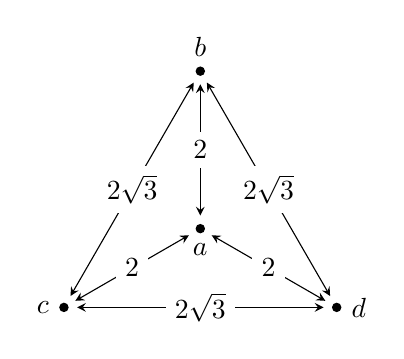
\begin{tikzpicture}[ >=stealth,
      dot/.style={circle,fill=black,inner sep=0,minimum size=1.2mm},
      len/.style={<->,shorten >=1mm,shorten <=1mm} ]
      % points
      \node[dot,label=below:{$a$}] (a) at (0,0) {};
      \node[dot,label=above:{$b$}] (b) at (90:2) {};
      \node[dot,label=left:{$c$}] (c) at (210:2) {};
      \node[dot,label=right:{$d$}] (d) at (330:2) {};

      % lengths
      \draw [len] (b) to (c);
      \draw [len] (c) to (d);
      \draw [len] (d) to (b);

      \draw [len] (a) to (b);
      \draw [len] (a) to (c);
      \draw [len] (a) to (d);      

      % labels
      \node[fill=white] at (270:1) {$2\sqrt{3}$};
      \node[fill=white] at (30:1) {$2\sqrt{3}$};
      \node[fill=white] at (150:1) {$2\sqrt{3}$};

      \node[fill=white] at (90:1) {$2$};
      \node[fill=white] at (210:1) {$2$};
      \node[fill=white] at (330:1) {$2$};
    \end{tikzpicture}
  \caption{A dataset in Euclidean space consisting of three points arranged in
  an equilateral triangle with another point at the centre.}
  \label{fig:points-in-plane}
\end{figure}

An all-squares optimal clustering, on the other hand, is not necessarily
linearly separable.  This can be shown by a simple example.  Consider a
dataset consisting of distinct points $a,b,c,d$ arranged in the Euclidean
plane as illustrated in Figure~\ref{fig:points-in-plane}.  There are $n$
copies of $a$ and one copy each of $b,c,d$.  The clustering $\clus =
\{\{(a,n)\},\{(b,1),(c,1),(d,1)\}\}$ has an all-squares cost of 72.  But if we
move one of $b,c,d$ into the first cluster, then we have a cost of $8n+24$
which is greater whenever $n>6$.  Similarly if we move two of $b,c,d$ into the
first cluster we get a cost of $16n+24$.  So whenever $n>6$ the all-squares
optimal clustering is $\clus$ and hence is not linearly separable.

% \subsection{Methods for finding optimal clusterings}
% \label{sec:meth-find-optim}

% In this paper we do not present any new methods for computing optimal
% clusterings, but we will briefly discuss existing methods and other
% possibilities here.  Optimal clustering is intuitively a hard problem.
% Centroid-distance clustering in Euclidean space was taken to be NP-complete
% for decades although this was proved only relatively
% recently\citep{aloise09exact}.  In the next section we will see that
% all-squares clustering is also NP-complete and for both problems we
% investigate the complexity for specific, very simple metric spaces.

% The consequence of the complexity of the problems is that heuristic algorithms
% for estimating optimal solutions are very prevalent; indeed, the $k$-means
% heuristic algorithm (also known as Lloyd's algorithm, although it was
% independently discovered by many different authors\citep{jain2010data}) for
% estimating the centroid-distance optimal $k$-clustering is probably the most
% well-known and widely-used clustering algorithm today.  Assuming that
% centroids are easy to compute, this algorithm is simple and, generally,
% quickly converges to a local optimum.  However, in the worst case, $k$-means
% requires exponentially many iterations in order to converge on a solution,
% even in the plane\citep{vattani2009exponential}.  There are many more
% heuristic methods for the problem; nine prominent methods are compared in
% \citep{brusco2007comparison}.

% Some algorithms for exactly solving the centroid-distance problem are known
% including methods using branch-and-bound \citep{brusco2006repetitive},
% branch-and-cut \citep{aloise09exact} and column generation
% \citep{merle1999interior}.  Some of these algorithms are able to exactly solve
% instances in the plane of around 2000 elements in reasonable time
% \citep{aloise09exact}.

% The all-squares problem, or more generally sum-of-cliques, has received less
% attention but there are, nonetheless, a number of algorithms described in the
% literature.  An exact algorithm using branch-and-bound
% \citep{klein1991optimal} can be used to solve problems with $n \leq 50, k \leq
% 5$ \citep{hansen1997mathprog}.  Cutting planes have also been applied with
% problems with $n \leq 158$ solved quickly
% \citep{hansen1997mathprog,palubeckis1997branch}.  In terms of heuristic
% approaches, there is an obvious iterative agglomerative technique that can be
% applied.  We have a simple randomised version that is showing some promise
% \citep{gk2012agglomerative}.

\section{Complexity issues}
\label{sec:complexity-issues}

We will now formally define the problems of finding an optimal clustering
according to either criteria and analyse the complexity of these problems.

\subsection{All-squares clustering}
\label{sec:all-squar-clust}

We state the all-squares problem formally as a decision problem:
\begin{problem}{All Squares Clustering (ASC)}
  \instance{A multiset of nodes $(\dset,\mu_{\dset})$, where $\dset =
    \{S_1,S_2,\dotsc,S_n\}$; a metric, $d$, which is defined for all elements
    in $\dset$; the number of clusters desired, $k \in \mathbb{Z}^+$ and a
    bound $B \in \mathbb{R}^+$.}  \question{Is there a $k$-clustering, $\clus
    = \{C_1,C_2,\dotsc,C_k\}$, such that
    \begin{equation*}
      cost_{as}(\clus)=
      \sum_{i=1}^{k} \sum_{x,y \in C_i} \mu_{C_i}(x)\mu_{C_i}(y)d^2(x,y)
      \leq B \quad \text{?}
    \end{equation*}}
\end{problem}

The problem is defined for multisets but, unless stated otherwise, the
NP-completeness proofs which follow are for sets, since this establishes the
result for multisets too.  When dealing with sets, the membership functions
are omitted since they are always equal to 1.

% so the cost function becomes simply
% \begin{equation*}
%   cost_{as}(\clus)=
%   \sum_{i=1}^{k} \sum_{x,y \in C_i} d^2(x,y).
% \end{equation*}

\subsubsection{Euclidean space}
\label{sec:euclidean-space}

An important special case of ASC is when the nodes are in Euclidean space and
we use the Euclidean metric $d_E$.  We call this special case Euclidean
all-squares clustering (EASC).

\begin{thm}
  EASC is NP-complete.
\end{thm}

\begin{proof}
  We observe that a guessed solution, $\clus_g$, can be checked in polynomial
  time by simply calculating $cost_{as}(\clus_g)$ and comparing the value to
  the bound.  Therefore $\text{EASC} \in \NP$.
  
  Now to show that EASC is NP-complete we construct a transformation from a
  known NP-complete problem to our problem.  The NP-complete problem we will
  use is the following \citep{gareyjohnson79}:
  \begin{problem}{Partition into Triangles (PT)}
    \instance{Graph $G = (V,E)$, with $|V| = 3q$ for some integer $q$.}
    \question{Can each of the vertices of $G$ be partitioned into $q$ disjoint
      sets $V_1,V_2,\dotsc,V_q$, each containing exactly $3$ vertices, such
      that for each $V_i = \{u_i,v_i,w_i\}, 1 \leq i \leq q$, all three of the
      edges $\{u_i,v_i\}, \{u_i,w_i\}$ and $\{v_i,w_i\}$ belong to $E$?}
  \end{problem}

  We transform an instance $I = G = (V,E)$ of PT, where $|V|=3p$, $V = \{v_0,
  \dotsc, v_{3p-1}\}$ and $|E|=m$ into an instance $f(I)$ of EASC: first we
  assign to $\dset$ a set of $n=3p$ points in $(3p+m)$-dimensional Euclidean
  space.  Each element $v_i \in V$ corresponds to a point where
  \begin{enumerate}
  \item the $i$th coordinate is $N = 2m$,
  \item all other coordinates $1 \leq i \leq 3p$ are 0,
  \item for $1 \leq j \leq m$, if $v_i$ is incident with $e_j \in E$ then the
    $(3p+j)$th coordinate is 1, otherwise it is 0.
  \end{enumerate}
  We then set $k$ to $p$ and $B$ to $8m-12p+12N^2p$.  It is easy to see that
  this transformation can be computed in polynomial time.

  \begin{lem}
    \label{lem:eq-dis}
    Let $\dset$ be a dataset with $|\dset| = n$ where the distance squared
    between each pair of distinct elements is $s$.  The sum-of-squares minimal
    $k$-clustering will contain clusters with cardinality of either
    $\left\lceil \frac{n}{k} \right\rceil$ or $\left\lfloor \frac{n}{k}
    \right\rfloor$ only.
  \end{lem}

  \begin{proof}
    The cost associated with a cluster, $C$, which contains $p$ elements is
    $p(p-1)s = (p^2-p)s$.  The extra cost of adding an element to $C$ is
    $((p+1)^2 - (p+1))s - (p^2-p)s = 2ps$, and the saving when removing an
    element is $(p^2 - p)s - ((p-1)^2 - (p-1))s = 2(p - 1)s$.

    We proceed by contradiction.  Assume that we have an optimal
    $k$-clustering, where $k \geq 2$ (the case where $k=1$ is trivial),
    including two clusters $C_i$ and $C_j$, where $|C_i| = p_i$, $|C_j| = p_j$
    and $p_i > p_j + 1$.  We move an element from $C_i$ to $C_j$; the
    difference in overall cost due to the move is $2p_js - 2p_is + 2s < 0$, so
    we have a saving.  Therefore our original clustering could not have been
    optimal.
  \end{proof}

  \begin{cor}
    \label{cor:extra-cost}
    Since $p_i \geq p_j + 2$, the difference in cost will be $(2p_j - 2p_i +
    2)s \leq 2s$.  Therefore, the cost of any suboptimal clustering will be at
    least $2s$ greater than the cost of the optimal clustering.
  \end{cor}

  In our reduction $\left\lceil \frac{n}{k} \right\rceil = \left\lfloor
    \frac{n}{k} \right\rfloor = 3$, so the optimal clustering when all nonzero
  distances are equal will be one where each cluster contains three elements.

  \begin{lem}
    \label{lem:euclidean-iff}
    $I$ is a YES instance of PT if and only if $f(I)$ is a YES instance of EASC.
  \end{lem}

  \begin{proof}
    If $I \in Y_{\text{PT}}$ then we can construct a clustering by letting
    each cluster correspond to one of the triangles in the partition of $G$.
    Let $w,x,y$ be the vertices of such a triangle, and therefore a cluster.
    The distance squared between a pair of these points is $d^2(w,x) =
    2N^2+\deg(w)+\deg(x)-2$; the $2N^2$ comes from the coordinates governed by
    rules 1 and 2 in the transformation and the $\deg(w) + \deg(x) - 2$ comes
    from the coordinates governed by rule 3.  The overall cost of the
    clustering is therefore $2(2\deg(w)+2\deg(x)+2\deg(y)+6N^2-6)$.  Hence,
    the set of $p$ triangles has cost
    \begin{equation}
      \label{eq:tri-cost}
      4\sum_{v \in V} \deg(v) + 12N^2p - 12p = 8m + 12N^2p - 12p = B,
    \end{equation}
    so $f(I) \in Y_{\text{EASC}}$.

    If $f(I) \in Y_{\text{EASC}}$ then we have a $k$-clustering which fits the
    bound.  The distance between each pair of distinct points in the dataset
    is at least $2N^2$.  Assume that the distances are all exactly $2N^2$: due
    to Lemma~\ref{lem:eq-dis}, the optimal clustering in this case is one
    where each cluster contains 3 elements, and this clustering has an overall
    cost of $12N^2p$.  Due to Corollary~\ref{cor:extra-cost}, any suboptimal
    clustering would have an overall cost of at least $(12p+4)N^2$ and, since
    $N^2=4m^2$, will not meet the bound.  Clearly, if one of these suboptimal
    clusterings contained distances greater than $2N^2$ in the sum their
    overall cost would be greater still.  Therefore, each cluster must contain
    exactly 3 elements.

    As shown in equation~\eqref{eq:tri-cost}, the cost of a clustering where
    each cluster corresponds to a triangle in $G$ equals the bound.  If some
    cluster does not correspond to a triangle, then its cost is increased, and
    therefore the overall cost of the clustering will be greater than the
    bound.  So each cluster must be a triangle, so $I \in Y_{\text{PT}}$.
  \end{proof}
  Hence, due to Lemma~\ref{lem:euclidean-iff}, the theorem is established.
\end{proof}

\subsubsection{$p$-valued metric}
\label{sec:p-valued-metric}

\begin{dfn}
  A \textbf{$p$-valued metric} is a metric where the cardinality of the
  codomain is equal to some positive integer $p$.
\end{dfn}

\begin{thm}
  \label{thm:np-complete-3-val}
  ASC is NP-complete even with a 3-valued metric.
\end{thm}

\begin{proof}
  We observe that a guessed solution can be checked in polynomial time,
  therefore $\text{ASC} \in \NP$.

  Now we choose again to construct a transformation from \textsc{Partition
    into Triangles} (PT).  An instance $I$ of PT is transformed into an
  instance $f(I)$ of ASC as follows: first we construct a 3-valued metric
  space by setting $\dset$ to $V$ and defining a function $d \colon \dset
  \times \dset \to \{0,\alpha,\beta\}$ where $0 > \alpha > \beta$ by
  \begin{equation*}
    d(u,v) = \begin{cases}
      0 & \text{if $u=v$,}\\
      \alpha & \text{if there exists an edge in $G$ between $u$ and $v$,}\\
      \beta & \text{otherwise.}
    \end{cases}
  \end{equation*}

  \begin{lem}
    \label{lem:3-val-met}
    $(\dset,d)$ is a metric space.
  \end{lem}
  
  \begin{proof}
    We show that $d$ satisfies each condition required for a metric for all
    $u,v,w \in \dset$:
    \begin{enumerate}
    \item $d(u,v)=0$ if and only if $u=v$ by definition,
    \item $d(u,v)=d(v,u)$ by definition,
    \item $d(u,v)+d(v,w) \geq d(u,w)$ (triangle inequality)\\
      If $u=w$ then this is trivially true.\\
      If $d(u,w)=\alpha$ then $u \neq w$ so either $u \neq v$ or $v \neq w$ or
      both.\\
      If $d(u,w)=\beta$ then $u \neq w$ and there is no edge between $u$ and
      $w$, we then have two cases: either both $u \neq v$ and $v \neq w$ which
      satisfies the inequality, or one of $u=v$ or $v=w$, but we know there is
      no edge between $u$ and $w$ so therefore there is no edge between $v$
      and $w$ or $v$ and $u$ respectively, so the inequality is satisfied.
    \end{enumerate}
  \end{proof}

  We then set $B$ to $6q\alpha$ and $k$ to $q$ to complete the transformation.
  It is easy to see that this transformation can be computed in polynomial
  time.

  \begin{lem}
    \label{lem:3-val-iff}
    $I$ is a YES instance of PT if and only if $f(I)$ is a YES instance of ASC.
  \end{lem}

  \begin{proof}
    If $I \in Y_{\text{PT}}$ then observe that we can construct a clustering,
    $\clus$, by assigning to each cluster $C_i$ the set $V_i$.  Since each
    $V_i$ has an edge between each pair of vertices, the cost of each cluster
    $C_i$ is $6\alpha$, and therefore the cost of $\clus$ is $6q\alpha$.  So
    therefore $f(I) \in Y_{\text{ASC}}$.

    If $I \in N_{\text{PT}}$ then we cannot have a clustering where all
    clusters have cardinality $3$ as this will contain at least one distance
    greater than $\alpha$ and therefore not meet the bound.  We must consider
    clusterings where all within cluster distances are equal to $\alpha$, but
    due to Lemma~\ref{lem:eq-dis}, any such clustering with clusters of
    different sizes always has a higher cost so they also cannot meet the
    bound.  Therefore $f(I) \in N_{\text{ASC}}$.
  \end{proof}

  Hence, due to Lemmata~\ref{lem:3-val-met} and \ref{lem:3-val-iff}, the
  theorem is established.

\end{proof}

\begin{thm}
  \label{thm:asc-np-complete-n-val}
  For all $n \geq 3$ there exists a metric such that ASC is hard, therefore
  ASC is NP-complete with an n-valued metric when $n \geq 3$.
\end{thm}

\begin{proof}
  We proceed by induction.  Theorem~\ref{thm:np-complete-3-val} establishes
  the base case, so we now assume that the problem is NP-complete with an
  $n$-valued metric and show that it is NP-complete with an $(n+1)$-valued
  metric.

  We transform an instance, $I$, of the $n$-valued problem into an instance,
  $f(I)$ of the $(n+1)$-valued problem.  Let $\dset^*$, $d^*$, $k^*$ and $B^*$
  be the dataset, metric, number of clusters and bound of $f(I)$,
  respectively.  We set $\dset^*$ to $\dset \cup \{a\}$, $k^*$ to $k+1$ and
  $B^*$ to $B$.  We define a function $d^* \colon \dset \times \dset$ by
  \begin{equation*}
    d^*(x,y) =
    \begin{cases}
      0 & \text{if $x=y$,}\\
      s & \text{if $x=a$ or $y=a$,}\\
      d(x,y) & \text{otherwise,}
    \end{cases}
  \end{equation*}
  where $s = \sum_{p,q \in \dset} d^2(p,q)$.  Notice that the distance between
  $a$ and each element in $\dset$ is the complete sum of all distances squared
  in $\dset$.  It is easy to see that this transformation can be computed in
  polynomial time.

  \begin{lem}
    \label{lem-asc-n-val-iff}
    $I$ is a YES instance of $n$-valued ASC if and only if $f(I)$ is a YES
    instance of $(n+1)$-valued ASC.
  \end{lem}
  \begin{proof}
    If $I \in Y_{ASC}$ then there is some clustering $\clus =
    \{C_1,C_2,\dotsc,C_k\}$ of $\dset$ with a cost less than or equal to $B$.
    We can construct a similar clustering of $\dset^*$ : $\clus^* = \clus \cup
    \{\{a\}\}$.  The extra cluster will not contribute to the cost, so the
    cost of $\clus^*$ is also less than or equal to $B$, so $f(I) \in
    Y_{ASC}$.

    If $f(I) \in Y_{ASC}$ then there is some clustering, $\clus^* =
    \{C^*_1,C^*_2,\dotsc, C^*_{k^*}\}$, with cost less than or equal to $B$.
    Let $C^*_l$ be the cluster which contains the element $a$.  If some other
    elements belong to this cluster then we can move them into any other
    cluster: each element we move makes a saving of at least $s^2$ but the
    final overall cost of the cluster we move them to can be at worst $s$, so
    clearly this will result in a saving.  Now, $C_l$ contains only $a$ so
    does not contribute to the overall cost, so $\clus^* \setminus C^*_l$ has
    an overall cost less than or equal to $B$ and therefore $I \in Y_{ASC}$.
  \end{proof}

  Hence, due to Lemma~\ref{lem-asc-n-val-iff}, the theorem is established.
\end{proof}

If our dataset is a set and the metric is 2-valued then the problem is
solvable in polynomial time due to Lemma~\ref{lem:eq-dis}.  We need only solve
the equation
\begin{equation*}
  x \left\lceil\frac{n}{k}\right\rceil
  + (k-x) \left\lfloor\frac{n}{k}\right\rfloor = n
\end{equation*}
for $x$ and an optimal clustering is then $x = n-k\lfloor\frac{n}{k}\rfloor$
clusters of $\lceil\frac{n}{k}\rceil$ elements and $k-x$ clusters of
$\lfloor\frac{n}{k}\rfloor$ elements.  For the decision version we would then
simply calculate the cost of the clustering to see if it is less than the
bound.  We conclude with:
\begin{thm}
  When the dataset is a set with a 2-valued metric, an optimal clustering can
  be found in polynomial time.
\end{thm}

However, if the dataset is a multiset this is not the case; the problem
becomes NP-complete.
\begin{thm}
  \label{thm:2-met-multiset-np-complete}
  When the dataset is a multiset with a 2-valued metric, ASC is an NP-complete
  problem.
\end{thm}

\begin{proof}
  We construct a transformation from the NP-complete problem
  \citep{gareyjohnson79}:
  \begin{problem}{Minimum Sum of Squares (MSS)}
    \instance{Finite set $A$, a size $s(a) \in \mathbb{Z}^+$ for each $a \in
      A$, positive integers $K \leq |A|$ and $J$.}
    \question{Can $A$ be partitioned into $K$ disjoint sets
      $A_1,A_2,\dotsc,A_k$ such that
      \begin{equation*}
        \sum_{i=1}^{K}\left(\sum_{a \in A_i} s(a)\right)^2 \leq J \quad ?
      \end{equation*}
    }
  \end{problem}
  We construct our dataset by setting $\dset$ to $A$ and $\mu_{\dset}$ to $s$
  and we set $k$ to $K$.  We define a metric $d$ for all $u,v \in \dset$ as
  \begin{equation*}
    d(u,v) =
    \begin{cases}
      0 & \text{if $u=v$,}\\
      1 & \text{otherwise.}
    \end{cases}
  \end{equation*}

  To find the value for $B$, consider an optimal multiset clustering
  $\clus=\{C_1,C_2,\dotsc,C_k\}$ which is consistent, so
  $\mu_{C_i}(x)=\mu_{\dset}(x)$ for all $x \in \dset$ and $1 \leq i \leq k$.
  The cost of a single cluster, $C_i$, is
  \begin{equation*}
    \sum_{x,y \in C_i} \mu_{\dset}(x)\mu_{\dset}(y)
    = \left(\sum_{x \in C_i} \mu_{\dset}(x)\right)^2
    - \sum_{x \in C_i} (\mu_{\dset}(x))^2,
  \end{equation*}
  so the total cost of $\clus$ is
  \begin{equation}
    \label{eq:clus-tot}
    \sum_{i=1}^{k}\left(\sum_{x \in C_i} \mu_{\dset}(x)\right)^2
    - \sum_{i=1}^{k}\sum_{x \in C_i} (\mu_{\dset}(x))^2.
  \end{equation}
  The second term is a constant and is equivalent to
  \begin{equation*}
    \Gamma = \sum_{x \in \dset} (\mu_{\dset}(x))^2.
  \end{equation*}
  We set $B$ to $J-\Gamma$ and the transformation is complete.  It is now easy
  to see that the cost of the optimal clustering, $\clus$, will meet the
  bound, $B$, if and only if the first term in expression~\eqref{eq:clus-tot}
  is less than or equal to $J$.  So $I \in Y_{\text{MSS}}$ if and only if
  $f(I) \in Y_{\text{ASC}}$ and the theorem is established.
\end{proof}

\subsection{Centroid-distance clustering}
\label{sec:centr-dist-clust}

Again, we state the problem formally as a decision problem:
\begin{problem}{Centroid-Distance Clustering (CDC)}
  \instance{A metric space $(M,d)$, a set of nodes $\dset \subseteq M$, the
    number of clusters desired, $k \in \mathbb{Z}^+$, and a bound, $B \in
    \mathbb{R}^+$.}
  \question{Is there a $k$-clustering, $\clus = \{C_1,C_2,\dotsc,C_k\}$ such
    that
    \begin{equation*}
      cost_{cd}(\clus)
      = \sum_{i=1}^{k} \sum_{x \in C_i} \mu_i(x) d^2(x,c_i) \leq B,
    \end{equation*}
    where $c_i \in M$ is the centroid of cluster $C_i$?
  }
\end{problem}
Again, the problem is defined for multisets, but the following proof is for
sets so the membership function has been omitted.

\begin{thm}
  \label{thm:CDC-NP}
  CDC is NP-complete.
\end{thm}

\begin{proof}
  We observe that a guessed solution, $\clus_g$, can be checked in polynomial
  time, therefore $\text{CDC} \in \NP$.

  To show that CDC is NP-complete we will construct a transformation from a
  known NP-complete problem to our problem.  The problem we will use is the
  following \cite{gareyjohnson79}:
  \begin{problem}{Dominating Set (DS)}
    \instance{A graph $G=(V,E)$ and a positive integer $K \leq |V|$.}
    \question{Is there a dominating set of size $K$ or less for $G$ or, in
      other words, a subset $V' \subseteq V$ with $|V'| \leq K$ such that for
      all $u \in V \setminus V'$ there is a $v \in V'$ for which $\{u,v\} \in
      E$?  }
  \end{problem}

  We transform an instance $I$ of DS into an instance $f(I)$ of CDC.  Fist we
  construct a 3-valued metric space by setting $M = \dset$ to $V$ and define a
  function $d \colon M \times M \to \rr$ by
  \begin{equation*}
    d(u,v) = \begin{cases}
      0 & \text{if $u=v$,}\\
      1 & \text{if there exists an edge in $G$ between $u$ and $v$,}\\
      2 & \text{otherwise.}
    \end{cases}
  \end{equation*}

  This is a metric space by Lemma~\ref{lem:3-val-met}. We then set $k$ to $K$
  and $B$ to $n-k$.

  \begin{lem}
    \label{lem:iff}
    $I$ is a YES instance of DS if and only if $f(I)$ is a YES instance of CDC.
  \end{lem}

  \begin{proof}
    If $I \in Y_{DS}$ then $|V'| \leq K = k$.  We can construct a
    $k$-clustering by first picking $k-|V'|$ arbitrary elements from $V
    \setminus V'$ and adding each of these to separate clusters.  These are
    final clusters and will not contribute to the overall cost.  We then add
    one element of the dominating set each to the remaining $|V'|$ clusters.
    These elements are the tentative centroids of the clusters.  So far we
    still have an overall cost of zero.  The remaining $n-k$ elements are
    added one by one to any cluster where they share an edge with the
    tentative centroid.  Thus, each of these $n-k$ elements contributes to the
    cost by 1.  If one of the final centroids of these constructed clusters
    turns out to be different to the tentative centroids, this can only
    decrease the cost of that cluster, by the definition of a centroid.
    Therefore the overall cost is less than or equal to $B = n-k$, so $f(I)
    \in Y_{CDC}$.

    \begin{figure}
      \centering
      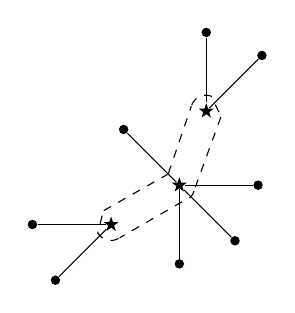
\begin{tikzpicture}[
        node/.style={circle,fill=black,inner sep=0,minimum size=1.2mm},
        cent/.style={star,star point height=0.6mm,fill=black,inner sep=0,minimum size=2mm},
        edge/.style={-},
        outl/.style={dashed},
        help/.style={inner sep=0,minimum size=0mm}]

        % dominating set nodes (centroids)
        \node[cent] (1) at (0,0) {};
        \node[cent] (2) at (70:1) {};
        \node[cent] (3) at (210:1) {};

        % other nodes
        \begin{scope}
          \node[node] (11) at (0:1) {};
          \node[node] (12) at (135:1) {};
          \node[node] (13) at (270:1) {};
          \node[node] (14) at (315:1) {};
          % helpers
          \node[help] (1h1) at (135:0.2) {};
          \node[help] (1h2) at (-20:0.2) {};
          \node[help] (1h3) at (300:0.2) {};
        \end{scope}
        
        \begin{scope}[shift={(70:1)}]
          \node[node] (21) at (45:1) {};
          \node[node] (22) at (90:1) {};
          % helpers
          \node[help] (2h1) at (-20:0.2) {};
          \node[help] (2h2) at (70:0.2) {};
          \node[help] (2h3) at (160:0.2) {};
        \end{scope}

        \begin{scope}[shift={(210:1)}]
          \node[node] (31) at (225:1) {};
          \node[node] (32) at (180:1) {};
          % helpers
          \node[help] (3h1) at (120:0.2) {};
          \node[help] (3h2) at (210:0.2) {};
          \node[help] (3h3) at (300:0.2) {};
        \end{scope}

        % edges
        \foreach \n in {11,12,13,14} {
          \draw [edge] (1) to (\n);
        }

        \foreach \n in {21,22} {
          \draw [edge] (2) to (\n);
        }

        \foreach \n in {31,32} {
          \draw [edge] (3) to (\n);
        }

        % dominating set outline
        \draw[outl] (1h1) -- (2h3) to [bend left=45] (2h2) to (2h1) -- (1h2)
        to [bend left=25] (1h3) -- (3h3) to [bend left=45] (3h2) to (3h1) -- (1h1);
      \end{tikzpicture}
      \caption{Each of the $k$ clusters correspond to star graphs with the
        centroid at the centre, so there is a dominating set of size $k$ as
        outlined.}
      \label{fig:domset}
    \end{figure}

    If $f(I) \in Y_{\text{CDC}}$ then we have an overall cost of less than or
    equal to $n-k$.  Since $\dset = M$, each cluster must contain an element
    equal to the centroid of that cluster, so there are exactly $k$ elements
    which do not contribute to the overall cost.  Each of the $n-k$ remaining
    elements must contribute to the cost by at least $1$, so therefore must
    contribute by exactly $1$ giving an overall cost of exactly $n-k$.  Each
    cluster therefore corresponds to a star in $G$, as illustrated in
    Figure~\ref{fig:domset}, so $I \in Y_{\text{DS}}$.
  \end{proof}

  Hence, due to Lemmata~\ref{lem:3-val-met} and \ref{lem:iff}, the theorem is
  established.
\end{proof}

Theorem~\ref{thm:CDC-NP} has already been established using Euclidean space.
In fact, the problem has been shown to be NP-hard for both $k=2$ in general
Euclidean space \citep{aloise09} and for general $k$ in only 2 dimensions
\citep{mahajan09}.  If both $k$ and $d$, the number of dimensions, are fixed,
the problem is exactly solvable in $O(n^{dk+1} \log n)$
time\citep{inaba94weightedvoronoi}.

Our proof establishes the following new result:
\begin{cor}
  Even if the metric, $d$, is a 3-valued metric, centroid-distance clustering
  remains an NP-complete problem.
\end{cor}

\begin{thm}
  \label{thm:cdc-np-complete-n-val}
  For all $n \geq 3$ there exists a metric such that CDC is hard, therefore
  CDC is NP-complete with an n-valued metric when $n \geq 3$.
\end{thm}

\begin{proof}
  We proceed by induction.  Theorem~\ref{thm:CDC-NP} establishes the base
  case, so we now assume that the problem is NP-complete with an $n$-valued
  metric and show that it is NP-complete with an $(n+1)$-valued metric.

  We use the same transformation as used for the proof of
  Theorem~\ref{thm:asc-np-complete-n-val}.

  \begin{lem}
    \label{lem-cdc-n-val-iff}
    $I$ is a YES instance of $n$-valued CDC if and only if $f(I)$ is a YES
    instance of $(n+1)$-valued CDC.
  \end{lem}

  \begin{proof}
    If $I \in Y_{CDC}$ then there is some clustering $\clus =
    \{C_1,C_2,\dotsc,C_k\}$ of $\dset$ with a cost less than or equal to $B$.
    We can construct a similar clustering of $\dset^*$: $\clus^* = \clus \cup
    \{\{a\}\}$.  The extra cluster will not contribute to the cost, so the
    cost of $\clus^*$ is also less than or equal to $B$, so $f(I) \in
    Y_{CDC}$.

    If $f(I) \in Y_{CDC}$ then there is some clustering $\clus^* =
    \{C^*_1,C^*_2,\dotsc,C^*_{k^*}\}$ which has cost less than or equal to
    $B$.  Let $C^*_l$ be the cluster which contains element $a$.  If other
    elements belong to this cluster then the cluster will have cost greater
    than or equal to $s^2$.  We can move all other elements to any other
    cluster, say $C^*_p$, which will reduce the cost of $C^*_l$ to 0, but the
    cost of $C^*_p$ must be less than $s$, so we have an overall saving.  Now
    $C^*_l$ does not contribute to the overall cost, so $\clus^* \setminus
    C^*_l$ has an overall cost less than or equal to $B$ and therefore $I \in
    Y_{CDC}$.
  \end{proof}
  Hence, due to Lemma~\ref{lem-cdc-n-val-iff}, the theorem is established.
\end{proof}

However, when the metric is 2-valued, the problem is solvable in polynomial
time, even in the multiset case.  To see this, let our metric be
\begin{equation*}
  d(u,v) =
  \begin{cases}
    0 & \text{if $u=v$,}\\
    s & \text{otherwise.}
  \end{cases}
\end{equation*}

The overall cost of a clustering will be
\begin{equation*}
  \sum_{i=1}^{k} \sum_{\{x \in C_i,x \neq c_i\}} \mu_{i}(x)s^2
\end{equation*}
or, equivalently,
\begin{equation*}
  \sum_{x \in \dset} \mu_{\dset}(x)s^2 - \sum_{i=1}^{k} \mu_{i}(c_i)s^2.
\end{equation*}
The first term is a constant, so the problem is to simply maximise the second
term.  This can be done by ordering the elements of $\dset$ by their
membership count in descending order and selecting the first $k$ elements.  We
move all copies of each of the selected elements to their own cluster; these
will become the centroids.  The remaining elements may then be moved to an
arbitrary cluster as they will all contribute to the cost by $s$ each in any
case.

\section{The assignment metric}
\label{sec:metr-comp-clust}

There are many existing methods for comparing clusterings.  Many do not
provide us with, or do not have established, bounds so are not very useful for
our purposes.  We will look at two metrics which have upper bounds: the
Variation of Information (VI) (see Section~\ref{sec:inform-theor}) and our
assignment metric which we present here.  The assignment metric is based on
set matching like those discussed in Section~\ref{sec:set-matching}, but
allows any metric to be used for comparing the matched sets.

Let $\mathcal{P}_k$ be the set of all possible $k$-clusterings of $\dset$.
We define the assignment metric as a function $\Delta \colon \mathcal{P}_k
\!\times \mathcal{P}_k \to \mathbb{R}$ where
\begin{equation*}
  \Delta(\clus_1, \clus_2) = \min_{\sigma \in S_k} \sum_{i=1}^{k}
  \delta(C_{1i}, C_{2\sigma(i)})
\end{equation*}
for some $\delta \colon (2^{\dset} \setminus \emptyset) \times (2^{\dset}
\setminus \emptyset) \to \mathbb{R}$ and where $S_k$ is the set of all
possible functions $\sigma \colon \{1, \dotsc, k\} \to \{1, \dotsc, k\}$.

\begin{thm}
  The measure $\Delta$ is a metric on $\mathcal{P}_k$ whenever $\delta$ is a
  metric on $(2^{\dset} \setminus \emptyset)$.
\end{thm}

\begin{proof}
  We show that $\Delta$ satisfies all conditions required for a metric:
  \begin{enumerate}
  \item $\Delta(\clus_1, \clus_2) \geq 0$ trivially since
    $\delta(C_{1i}, C_{2j}) \geq 0$ for all $1 \leq i,j \leq k$ since
    $\delta$ is itself a metric,
  \item If $\clus_1 = \clus_2$ then there exists some $\sigma$ for which
    $C_{1i} = C_{2\sigma(i)}$ and therefore $\delta(C_{1i},
    C_{2\sigma(i)}) = 0$ for all $1 \leq i \leq k$, so $\Delta(\clus_1,
    \clus_2) = 0$.

    If $\Delta(\clus_1, \clus_2) = 0$ then $\delta(C_{1i},
    C_{2\sigma(i)}) = 0$ and therefore $C_{1i} = C_{2\sigma(i)}$ for
    some $\sigma$ and all $1 \leq i \leq k$, so $\clus_1 = \clus_2$,
  \item $\Delta(\clus_1, \clus_2) = \Delta(\clus_2, \clus_1)$
    trivially since $\delta(C_{1i}, C_{2j}) = \delta(C_{2j}, C_{1i})$
    for all $1 \leq i,j \leq k$,
  \item Let $\Delta(\clus_1, \clus_2) = \sum_{i=1}^{k} \delta(C_{1i},
    C_{2\sigma(i)})$ for
    some $\sigma \in S_k$\\
    and $\Delta(\clus_2, \clus_3) = \sum_{i=1}^{k} \delta(C_{2i},
    C_{\uptau(i)})$ for some $\uptau \in S_k$.
    
    Then,
    \vspace{-1em}
    \begin{align*}
      \Delta(\clus_1, \clus_2) + \Delta(\clus_2, \clus_3) &=
      \sum_{i=1}^{k} \delta(C_{1i},
      C_{2\sigma(i)}) + \delta(C_{2\sigma(i)}, C_{3\uptau(\sigma(i))})\\
      &\geq \sum_{i=1}^{k} \delta(C_{1i},
      C_{3\uptau(\sigma(i))})\quad\text{(due to
        triangle inequality of $\delta$)}\\
      &\geq \min_{\sigma \in S_k} \sum_{i=1}^{k} \delta(C_{1i}, C_{3\sigma(i)})\\
      &= \Delta(\clus_1, \clus_3).
    \end{align*}
  \end{enumerate}
\end{proof}

Possible choices for the $\delta$ metric are the cardinality of the symmetric
difference, $\delta(A,B) = |A \symdif B|$, and the normalised symmetric
difference, also known as the Jaccard distance, $\delta(A,B) = \frac{|A
  \symdif B|}{|A \cup B|}$.  These are well known metrics with the former
being used often in the literature for comparing sets, for example in
\cite{reynolds2006clustering}.  These two metrics extend naturally to
multisets; the multiset version of symmetric difference is
$\delta((A,\mu_A),(B,\mu_B)) = \sum_{x,y \in A \cup B} |\mu_A(x)-\mu_B(y)|$.

Calculating $\Delta$ amounts to calculating the minimum cost matching between
the clusters.  There are $k!$ possible matchings, but the minimum can be found
in $O(k^3)$ time using the Hungarian algorithm \cite{kuhn1955hungarian}.
Since $k! < k^3$ when $k < 6$, it may be more efficient to simply enumerate
all solutions when $k$ is small.

Clusterings with different $k$ can be compared by the addition of the
pseudometric $||\clus_1|-|\clus_2||$ (ie. the absolute difference between the
set cardinalities).  Let $\mathcal{P}$ be the set of all partitions of
$\dset$.  The assignment metric then becomes a function $\Delta \colon
\mathcal{P} \times \mathcal{P} \to \mathbb{R}$ defined as
\begin{equation*}
  \Delta(\clus_1, \clus_2)
  = \min_{\sigma \in S_k} \sum_{i=1}^{k} \delta(C_{1i},C_{2\sigma(i)})
  + \lambda ||\clus_1|-|\clus_2||,
\end{equation*}
where $k = \min(|C_1|,|C_2|)$, $\delta \colon (2^{\dset}\setminus \emptyset)
\times (2^{\dset}\setminus \emptyset) \to \mathbb{R}$ and $\lambda$ is a
positive real number.

This is most sensible when the metric $\delta$ is bounded or normalised and
$\lambda$ is greater than or equal to the upper bound on $\delta$.
Calculation of the metric using the Hungarian algorithm can then be performed
by a simple modification, namely by setting the cost of matching a set to
nothing as $\lambda$ and finding the minimum matching in the same way.

Using a bounded metric does not limit our choice since any metric can be
bounded.  One general formula for bounding a metric by $[0,1]$ is
\begin{equation}
  \label{eq:met-bound}
  \delta_b (A,B) = \frac{\delta(A,B)}{1+\delta(A,B)}.
\end{equation}
Alternatively, it may be possible to normalise the metric, as with the
normalised symmetric difference metric.

This version of the assignment metric is bounded by $\lambda \cdot
\max(|\clus_1|,|\clus_2|)$, and this bound is approached arbitrarily closely
by $\clus_1 = \{\{1,2,\dotsc,n\}\}, \clus_2 = \{\{1\},\{2\},\dotsc,\{n\}\}$ in
the limit of large $n$ for any metric $\delta$.  Tighter bounds may exist for
specific choices of $\delta$ and fixed $k$ (we prove one in
Section~\ref{sec:upper-bound}).

In Section~\ref{sec:asgn-met-fuzzy-partitions} we show how the assignment
metric can be used to compare fuzzy partitions and in
Section~\ref{sec:lifting-metric-space} we discuss the use of metrics which are
aware of the underlying metric space of a clustering.  In
Section~\ref{sec:worst-case-perf} we use the symmetric difference to prove a
worst case result for our two clustering criteria.

\subsection{Comparing fuzzy partitions}
\label{sec:asgn-met-fuzzy-partitions}

The assignment metric extends easily to fuzzy partitions.  All we need is a
metric on fuzzy sets.  Here we present such a metric which is analogous to the
symmetric difference.

Let $\mathcal{F}_f$ be the set of all fuzzy sets and $\mathcal{F}_c \subset
\mathcal{F}_f$ the set of all crisp sets.  Note that a crisp set is a special
case of a fuzzy set where
\begin{equation*}
  \mu_A(x) =
  \begin{cases}
    1 & \text{if $x \in A$}\\
    0 & \text{if $x \notin A$}
  \end{cases}
\end{equation*}
for all $A \in \mathcal{F}_c$.

We now define a function $\delta_f \colon \mathcal{F}_f \times \mathcal{F}_f
\to \mathbb{R}$ by
\begin{equation*}
  \delta_f(A,B) = \sum_{x \in \mathcal{R}} |\mu(x,A) - \mu(x,B)|.
\end{equation*}

\begin{thm}
  The measure $\delta_f$ is equivalent to the symmetric difference
  $\delta(A,B) = |A \symdif B|$ for all $A,B \in \mathcal{F}_c$.
\end{thm}

\begin{proof}
  For each $x \in \mathcal{R}$:
  \begin{enumerate}
  \item If $x \notin A$ and $x \notin B$ then $\mu(x,A) = \mu(x,B) = 0$ and
    therefore this does not contribute to the sum in $\delta_f(A,B)$,
  \item if $x \in A$ and $x \notin B$ then $\mu(x,A) = 1$ and $\mu(x,B) = 0$
    so $|\mu(x,A) - \mu(x,B)| = |1 - 0| = 1$,
  \item similarly, if $x \notin A$ and $x \in B$ then $|\mu(x,A) - \mu(x,B)|
    = |0 - 1| = 1$,
  \item if $x \in A$ and $x \in B$ then $|\mu(x,A) - \mu(x,B)| = |1 - 1| = 0$
    and therefore also does not contribute to the sum.
  \end{enumerate}
\end{proof}

For fuzzy sets this measure does correspond to $|A \symdif B| = |A \cup B|
- |A \cap B|$ since
\begin{align*}
  \mu(x, A \cup B) &= \max(\mu(x,A), \mu(x,B))\\
  \mu(x, A \cap B) &= \min(\mu(x,A), \mu(x,B))
\end{align*}
so the cardinality $|A \cup B| - |A \cap B|$ is
\begin{align*}
  &\sum_{x \in \mathcal{R}} \big(\max(\mu(x,A),\mu(x,B)) - \min(\mu(x,A),\mu(x,B))\big)\\
  &= \sum_{x \in \mathcal{R}} |\mu(x,A) - \mu(x,B)|
\end{align*}

\begin{thm}
  $(\mathcal{F}_f, \delta_f)$ is a metric space.
\end{thm}

\begin{proof}~
  
  \begin{enumerate}
  \item $\delta_f(A,B) = 0 \iff A=B$:
    \begin{align*}
      \delta_f(A,B) = 0 &\iff \mu(x,A) = \mu(x,B) \quad \forall x \in
      \mathcal{R}\\
      &\iff A = B,
    \end{align*}
  \item $\delta_f(A,B) = \delta_f(B,A)$ by definition,
  \item $\delta_f(A,B)+\delta_f(B,C) \geq \delta_f(A,C)$ (the triangle
    inequality):
    \begin{align*}
      \delta_f(A,B) + \delta_f(B,C)
      &= \sum_{x \in \mathcal{R}} |\mu(x,A) - \mu(x,B)|
      + \sum_{x \in \mathcal{R}} |\mu(x,B) - \mu(x,C)|\\
      &= \sum_{x \in \mathcal{R}} \big(|\mu(x,A)-\mu(x,B)|
      + |\mu(x,B)-\mu(x,C)|\big)\\
      &\geq \sum_{x \in \mathcal{R}} |\mu(x,A) - \mu(x,C)|\\
      &= \delta_f(A,C)
    \end{align*}
  \end{enumerate}
\end{proof}

There is also a corresponding normalised version of this metric for use with
the second version of the assignment metric:
  \begin{equation*}
    \delta_{f_n}(A,B) = \frac{|A \symdif B|}{|A \cup B|}.
  \end{equation*}

\subsection{Lifting the underlying metric space}
\label{sec:lifting-metric-space}

\begin{figure}
  \centering
  \begin{subfigure}[b]{0.3\textwidth}
    \begin{tikzpicture}
      \begin{axis}[xmin=0,xmax=10,ymin=0,ymax=10,width=1.2\textwidth,tick label style={font=\tiny}]
        \addplot+[only marks,color=blue,mark=o] table {
          2.0 2.0
          1.0 2.0
          2.0 1.0
          0.9 2.3
          2.1 0.7
          1.4 1.3
          2.6 2.8
          2.3 1.2
          3.6 2.1
          4.6 2.4
          3.6 2.5
          3.4 1.2
        };
        \addplot+[only marks,color=red,mark=x] table {
          8.0 2.0
          6.2 2.6
          8.8 3.9
          7.6 2.4
          7.2 3.2
          5.6 2.0
          8.7 2.4
          8.9 1.5
          7.0 2.0
          6.5 1.7
          7.3 1.6
          5.8 1.5
        };
        \addplot+[only marks,color=brown,mark=triangle] table {
          5.0 8.0
          5.5 8.6
          5.7 7.2
          5.2 6.2
          6.8 8.2
          5.2 6.7
          3.8 9.2
          3.7 8.2
          4.3 6.2
          4.9 6.7
          5.0 9.0
          4.5 8.6
        };
      \end{axis}
    \end{tikzpicture}
    \caption{Clustering $\clus_1$.}
    \label{fig:clus1}
  \end{subfigure}
  \begin{subfigure}[b]{0.3\textwidth}
    \begin{tikzpicture}
      \begin{axis}[xmin=0,xmax=10,ymin=0,ymax=10,width=1.2\textwidth,tick label style={font=\tiny}]
        \addplot+[only marks,color=blue,mark=o] table {
          2.0 2.0
          1.0 2.0
          2.0 1.0
          0.9 2.3
          2.1 0.7
          1.4 1.3
          2.6 2.8
          2.3 1.2
          3.6 2.1
          4.6 2.4
          3.6 2.5
          3.4 1.2
          5.2 6.2
          4.3 6.2
          4.9 6.7
          5.2 6.7        
        };
        \addplot+[only marks,color=red,mark=x] table {
          8.0 2.0
          6.2 2.6
          8.8 3.9
          7.6 2.4
          7.2 3.2
          5.6 2.0
          8.7 2.4
          8.9 1.5
          7.0 2.0
          6.5 1.7
          7.3 1.6
          5.8 1.5
        };
        \addplot+[only marks,color=brown,mark=triangle] table {
          5.0 8.0
          5.5 8.6
          5.7 7.2
          6.8 8.2
          3.8 9.2
          3.7 8.2
          5.0 9.0
          4.5 8.6
        };
      \end{axis}
    \end{tikzpicture}
    \caption{Clustering $\clus_2$.}
    \label{fig:clus2}
  \end{subfigure}
  \begin{subfigure}[b]{0.3\textwidth}
    \begin{tikzpicture}
      \begin{axis}[xmin=0,xmax=10,ymin=0,ymax=10,width=1.2\textwidth,tick label style={font=\tiny}]
        \addplot+[only marks,color=blue,mark=o] table {
          2.0 2.0
          1.0 2.0
          2.0 1.0
          0.9 2.3
          2.1 0.7
          1.4 1.3
          2.6 2.8
          2.3 1.2
          3.6 2.1
          4.6 2.4
          3.6 2.5
          3.4 1.2
          
          6.2 2.6
          5.6 2.0
          6.5 1.7
          5.8 1.5
        };
        \addplot+[only marks,color=red,mark=x] table {
          8.0 2.0
          8.8 3.9
          7.6 2.4
          7.2 3.2
          8.7 2.4
          8.9 1.5
          7.0 2.0
          7.3 1.6
        };
        \addplot+[only marks,color=brown,mark=triangle] table {
          5.0 8.0
          5.5 8.6
          5.7 7.2
          5.2 6.2
          6.8 8.2
          5.2 6.7
          3.8 9.2
          3.7 8.2
          4.3 6.2
          4.9 6.7
          5.0 9.0
          4.5 8.6
        };
      \end{axis}
    \end{tikzpicture}
    \caption{Clustering $\clus_3$.}
    \label{fig:clus3}
  \end{subfigure}
  \caption{Three clusterings on the same dataset.}
  \label{fig:three-clusterings}
\end{figure}


Another possibility that the assignment metric gives us is to use a metric
which is aware of the metric space underlying our clustering.  This overcomes
some of the limitations that are present in most comparison methods
\citep{bae2010comparison}.

Figure~\ref{fig:three-clusterings} shows three possible clusterings,
$\clus_1,\clus_2$ and $\clus_3$ on a given dataset.  The elements in this
dataset exist in the Euclidean plane and are shown in their relative positions
on the page.  Imagine that $\clus_1$ represents the standard clustering and
$\clus_2$ and $\clus_3$ are two alternative clusterings.  We would like to
know which of the alternative clusterings is closest to the standard so we
measure the distance between $\clus_1$ and $\clus_2$ and $\clus_1$ and
$\clus_3$.  Under the VI metric we get $\Delta(\clus_1,\clus_2) =
\Delta(\clus_1,\clus_3) = 3.1154556$.  Under the assignment metric with the
symmetric difference we similarly get $\Delta(\clus_1,\clus_2) =
\Delta(\clus_1,\clus_3) = 72$.  This seems contrary to our intuition: we would
expect that $\clus_2$ is further from the standard since the clusters are of
very different shapes.  The assignment metric combined with the Hausdorff
metric $\delta_{H}$ and Euclidean metric $d_E$ reflects this intuition: we get
$\Delta(\clus_1,\clus_2) = 6.0621233$ and $\Delta(\clus_1,\clus_3) =
3.424846$.  We could, of course, have used a metric other than the Euclidean
metric to plug in to the Hausdorff metric if this made more sense.

The Hausdorff metric can be normalised in a natural way for use with the
second version of the assignment metric.  One way would be to divide by the
maximum distance observed in the dataset:
\begin{equation*}
  \delta_{H_n}(X,Y) = \frac{\delta_{H}(X,Y)}{\max_{x,y \in \dset} d(x,y)}.
\end{equation*}

When we use a metric like the Hausdorff metric we have three ``layers'' of
metric space that we are dealing with.  The underlying layer is our dataset
and metric used for clustering $(\dset, d)$.  We have the cluster layer
$(2^{\dset} \setminus \emptyset,\delta)$ and the clustering layer
$(\mathcal{P},\Delta)$.  When we take into account all three layers we say
that we are ``lifting'' the underlying metric space to the space of
partitions.

% Distances between c1 and c2 and c1 and c3 resp.

% VI
% 3.1154556  3.1154556
% asgn met - symdif
% 72
% asgn met - hausdorff
% 6.0621233  3.424846

It should be noted that two commonly used functions for comparing sets in a
metric space
\begin{equation*}
  f_1(X, Y) = \min_{x \in X, y \in Y} d(x, y)
\end{equation*}
and
\begin{equation*}
  f_2(X, Y) = \sum_{x \in X} \sum_{y \in Y} d(x, y)
\end{equation*}
are \textit{not} metrics.  This can be shown by considering a simple
counterexample for each: $f_1(\{x,y\},\{x,z\}) = 0$ violates property 3 of a
metric (identity of indiscernibles) and $f_2(\{x,y\},\{x,y\}) > 0$ violates
property 2 (identical elements are most similar).

\subsection{Upper bound}
\label{sec:upper-bound}

An upper bound for $\Delta$ can be established when $\delta(A,B) = |A \symdif
B|$.  We show the upper bound using sets for clarity, but the result is still
valid for multisets using the multiset version of symmetric difference.

There are $k^2$ possible matchings between clusters, the costs of which can be
shown in a matrix:
\begin{equation*}
  \begin{pmatrix}
    |C_{11} \symdif C_{21}| & |C_{12} \symdif C_{21}|
    & \dots & |C_{1k} \symdif C_{21}| \\
    |C_{11} \symdif C_{22} | & |C_{12} \symdif C_{22} |
    & \dots & |C_{1k} \symdif C_{22} | \\
    \vdots & \vdots & \ddots & \vdots \\
    |C_{11} \symdif C_{2k} | & |C_{12} \symdif C_{2k} |
    & \dots & |C_{1k} \symdif C_{2k} |
  \end{pmatrix}.
\end{equation*}
Let $p_i = |C_{1i}|$, $p_j = |C_{2j}|$ and $p_{ij} = |C_{1i} \cap C_{2j}|$.
We can calculate the sum of the values in the $j$th row of the matrix for some
$j$:
\begin{align*}
  \sum_{i=1}^{k} |C_{1i} \symdif C_{2j}| &= \sum_{i=1}^{k} (|C_{1i} \cup
  C_{2j}| - | C_{1i} \cap C_{2j}|) \\
  &= \sum_{i=1}^{k} (p_j + p_i - 2p_{ij}).
\end{align*}
Noting that $\sum_{i=1}^{k} p_i = m$ and $\sum_{i=1}^{k} p_{ij} = p_j$ this
can be written as
\begin{equation*}
  kp_j + m - 2p_j = (k-2)p_j + m.
\end{equation*}
The total sum of values in the matrix is therefore
\begin{equation*}
  \sum_{j=1}^{k} ((k-2)p_j + m),
\end{equation*}
and noting that $\sum_{j=1}^{k} p_j = m$ we get
\begin{equation*}
  (k-2)m + mk.
\end{equation*}

There are $k!$ possible solutions to the assignment problem where each
solution is a combination of $k$ assignments.  Let $S = \{s_1, s_2, \dotsc,
s_{k!}\}$ be the set of costs for each solution so each element is equal to
$\sum_{i=1}^{k} \delta(C_{1i}, C_{2\sigma(i)})$ for some $\sigma$.  The mean
value in the matrix is
\begin{equation*}
  \frac{(k-2)m + mk}{k^2},
\end{equation*}
so the mean solution value is
\begin{align*}
  \bar{s} &= k \left( \frac{(k-2)m + mk}{k^2} \right)\\
          &= 2m - \frac{2m}{k}.
\end{align*}

We can split $S$ into three disjoint subsets $S_{<}$, $S_{=}$ and $S_{>}$
which contain the solutions which are less than, equal to and greater than the
mean, respectively.  We have two cases: either both $S_{<} = \emptyset$ and
$S_{>} = \emptyset$ or both $S_{<} \neq \emptyset$ and $S_{>} \neq \emptyset$.
In the first case, all solutions are equal to the mean and therefore any of
these will be picked; in the second case, a solution from $S_{<}$ will be
picked.

\begin{figure}
  \centering
  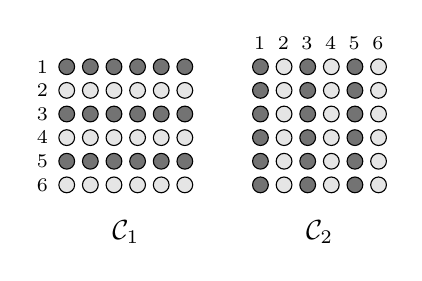
\begin{tikzpicture}[
    poi/.style={circle,draw=black,inner sep=0,minimum size=2mm}
    ]

    % clustering one
    \foreach \y in {0,0.6,1.2} {
      \foreach \x in {0,0.3,0.6,0.9,1.2,1.5} {
        \node[poi,fill=gray!110] at (\x,\y+0.3) {};
        \node[poi,fill=gray!20] at (\x,\y) {};
      }
    }
    % cluster labels
    \foreach \y/\n in {1.5/1,1.2/2,0.9/3,0.6/4,0.3/5,0/6} {
      \node at (-0.3,\y) {$_\n$};
    }

    % clustering label
    \node at (0.75,-0.6) {$\clus_1$};

    % clustering two
    \begin{scope}[xshift=70]
      \foreach \y in {0,0.3,0.6,0.9,1.2,1.5} {
        \foreach \x in {0,0.6,1.2} {
          \node[poi,fill=gray!20] at (\x+0.3,\y) {};
          \node[poi,fill=gray!110] at (\x,\y) {};
        }
      }

      % cluster labels
      \foreach \x/\n in {1.5/6,1.2/5,0.9/4,0.6/3,0.3/2,0/1} {
        \node at (\x,1.8) {$_\n$};
      }

      % clustering label
      \node at (0.75,-0.6) {$\clus_2$};
    \end{scope}

  \end{tikzpicture}
  \caption{Two clusterings, $\clus_1$ and $\clus_2$, formed of six
    clusters each.  These clusterings are optimally different under both the
    assignment metric and variation of information.}
  \label{fig:worst-case}
\end{figure}

Therefore
\begin{equation*}
  \Delta(\clus_1,\clus_2) \leq 2m - \left\lceil \frac{2m}{k} \right\rceil.
\end{equation*}
This bound is tight and can be met with the worst case
\begin{align*}
  \clus_1 = \{&\{1,\dotsc,k\},\{k+1,\dotsc,2k\},\dotsc,\{(k-1)k+1,\dotsc,k^2\}\} \\
  \clus_2 = \{&\{1,k+1,\dotsc,(k-1)k+1\},\\
  &\{2,k+2,\dotsc,(k-1)k+2\},\\
  &\dotsc,\\
  &\{k,k+k,\dotsc,(k-1)k+k\}\}
\end{align*}
which is also shown in Figure~\ref{fig:worst-case}.  This also produces the
worst case under the VI metric, as shown in \citep{meila-2007}.

\section{Worst case performance}
\label{sec:worst-case-perf}

We have so far seen that our two clustering criteria have a number of
similarities, and a number of differences.  Using our metrics for comparing
clusterings, we will now show just how different an all-squares optimal
clustering and a centroid-distance optimal clustering of the same dataset can
be.

\begin{figure}
  \centering
  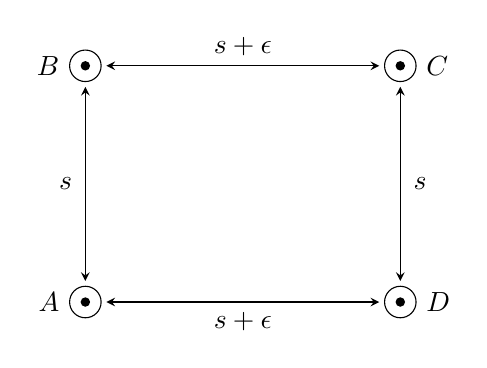
\begin{tikzpicture}[
    >=stealth,
    dot/.style={circle,fill=black,inner sep=0,minimum size=1.2mm},
    sur/.style={circle,fill=white,draw=black,inner sep=0,minimum size=4mm},
    len/.style={<->,shorten >=2mm,shorten <=2mm}
    ]
    % surrounds
    \node[sur,label=left:{$A$}] (A) at (0,0) {};
    \node[sur,label=left:{$B$}] (B) at (0,3) {};
    \node[sur,label=right:{$C$}] (C) at (4,3) {};
    \node[sur,label=right:{$D$}] (D) at (4,0) {};

    % dots
    \node[dot] (A) at (0,0) {};
    \node[dot] (B) at (0,3) {};
    \node[dot] (C) at (4,0) {};
    \node[dot] (D) at (4,3) {};

    % length arrows
    \draw [len] (A) to (B);
    \draw [len] (B) to (D);
    \draw [len] (D) to (C);
    \draw [len] (C) to (A);

    % length labels
    \node at (-0.25,1.5) {$s$};
    \node at (4.25,1.5) {$s$};

    \node at (2,-0.25) {$s+\epsilon$};
    \node at (2,3.25) {$s+\epsilon$};
  \end{tikzpicture}
  \caption{Relative positions of elements to be clustered.  $A$ and $B$
    contain $N$ elements each, $C$ and $D$ contain $N+1$ elements each.}
  \label{fig:clusters}
\end{figure}

Let $(M,d_E)$ be 2-dimensional Euclidean space with the Euclidean metric and
our dataset be $(\dset, \mu_{\dset})$ where $\dset \subset \mathbb{R}^2$,
$\dset = A \cup B \cup C \cup D$, $\mu_{\dset}(A)=\mu_{\dset}(B)=N$ and
$\mu_{\dset}(C)=\mu_{\dset}(D)=N+1$.  The relative positions of $A,B,C,D$ in
the Euclidean plane are shown in Figure~\ref{fig:clusters}.  Two possible
$2$-clusterings of $(\dset,\mu_{\dset})$ are $\{A \cup B,C \cup D\}$ and $\{A
\cup D,B \cup C\}$ which we will call $\clus_1$ and $\clus_2$ respectively.

Formulae for the all-squares and centroid-distance costs of $\clus_1$ and
$\clus_2$ can now be given, first for centroid-distance cost:
\begin{eqnarray*}
  cost_{cd}(\clus_1) &=& \frac{1}{2}\left(Ns^2+(N+1)s^2\right), \\
  cost_{cd}(\clus_2) &=& \frac{1}{2}\left(N(s+\epsilon)^2+(N+1)(s+\epsilon)^2\right).
\end{eqnarray*}
It is clear that $\clus_1$ is the optimal clustering under the
centroid-distance criterion whenever $\epsilon > 0$.  Now, for all-squares
cost,
\begin{eqnarray*}
  cost_{as}(\clus_1) &=& 2N^2s^2+2(N+1)^2s^2, \\
  cost_{as}(\clus_2) &=& 4N(N+1)(s+\epsilon)^2.
\end{eqnarray*}
So $\clus_2$ is the optimal clustering under the all-squares criterion
whenever
\begin{equation*}
  \epsilon < \sqrt{s^2 + \frac{s^2}{2N(N+1)}} - s.
\end{equation*}
Other clusterings of $\dset$ are possible, but these are trivially more
expensive.

A simple numerical example can now be constructed; let $s=1.4$, $\epsilon=0.1$
and $N=1$.  The costs of all possible 2-clusterings are shown in
Table~\ref{tab:costs}.  Again we see that the optimal clustering under each
criterion is different.

% \begin{table}
%   \centering
%   \caption{The costs of possible 2-clusterings
%     of $\dset$, with minimum costs underlined.}
%   \begin{tabular}{lrr}
%   \toprule
%   Clustering & Centroid-distance cost & All-squares cost \\
%   \midrule
%   $\{A \cup B, C \cup D\}$ & \underline{2.94} & 19.6 \\
%   $\{A \cup D, B \cup C\}$ & 3 & \underline{18} \\
%   $\{A \cup C, B \cup D\}$ & $5\frac{46}{75}$ & 33.68 \\
%   $\{A, B \cup C \cup D\}$ & 4.152 & 41.52 \\
%   $\{C, A \cup B \cup D\}$ & 4.2825 & 29.76 \\
%   \bottomrule
% \end{tabular}
% \label{tab:costs}
% \end{table}

\begin{table}
  \centering
  \caption{The costs of possible 2-clusterings
    of $\dset$, with minimum costs underlined.}
  \begin{tabular}{lrr}
  \toprule
  Clustering & Centroid-distance cost & All-squares cost \\
  \midrule
  $\{A \cup B, C \cup D\}$ & \underline{2.940} & 19.60 \\
  $\{A \cup D, B \cup C\}$ & 3.375 & \underline{18.00} \\
  $\{A \cup C, B \cup D\}$ & 5.613 & 33.68 \\
  $\{A, B \cup C \cup D\}$ & 4.152 & 41.52 \\
  $\{B, A \cup C \cup D\}$ & 4.152 & 41.52 \\
  $\{C, A \cup B \cup D\}$ & 4.283 & 29.76 \\
  $\{D, A \cup B \cup C\}$ & 4.283 & 29.76 \\
  \bottomrule
\end{tabular}
\label{tab:costs}
\end{table}


$\clus_1$ and $\clus_2$ are not just slightly different clusterings, they are
in fact optimally different, that is, no two clusterings can be more
different, according to both the VI metric and assignment metric, as well as
our basic intuition.  This leads us to:
\begin{thm}
  \label{thm:worst-case}
  A centroid-distance optimal clustering and an all-squares optimal clustering
  can be optimally different under both the VI metric and the assignment
  metric.
\end{thm}

\section{Conclusion}
\label{sec:conclusion}

In this chapter we have shown that the two sum-of-squares criteria,
centroid-distance and all-squares, share some similarities but also some
differences.  Optimal clusterings according to both criteria may be consistent
but, while centroid-distance always produces linearly separable solutions,
all-squares does not.

Both criteria simultaneously measure both homogeneity and separation.  For
all-squares, the relationship between the homogeneity measure and separation
measure is trivial and independent of the choice of metric.  However, for
centroid-distance we have shown that the homogeneity measure is not
necessarily equivalent to the separation measure when using something other
than the Euclidean metric.  The example we used is the homogeneous
Euclidean-overlap metric for mixed data.

It has recently been shown that the centroid-distance problem is NP-hard using
Euclidean space.  We have shown that both problems are NP-complete even when
using a simple 3-valued metric.  We also show that all-squares is NP-complete
in Euclidean space.  When using a 2-valued metric, both problems are in P,
except for all-squares on a multiset, which remains NP-complete.

We have introduced a new metric for comparing clusterings, called the
assignment metric.  It is, in fact, a family of metrics since any metric for
comparing matched sets can be used.  This allows for some interesting choices
of metric, namely we can use it to compare fuzzy clusterings and take into
account the underlying metric space of the dataset which gives the measure a
more intuitive feel.

We have used this metric to show just how different optimal clusterings
according to the two criteria can be.  It turns out that they can be optimally
different, according to both our metric and the VI metric.

Much of the work here which we present for multisets also applies naturally to
fuzzy multisets.  The consistency results also extend to crispness, that is to
say that optimal fuzzy clusterings according to either criteria need not have
been fuzzy in the first place.  The assignment metric also applies to fuzzy
clusterings simply by using a metric for fuzzy sets.

% Further work will be done on methods for approximating the optimal clustering
% according to all-squares.  Further applications for the assignment metric and
% new bounds will also be investigated.



%%% Local Variables:
%%% TeX-master: "thesis"
%%% End:


\chapter{Hierarchical Clustering}
\label{cha:background2}

\section{Summary}
\label{sec:summary}

In this section we review the relevant terminology and background that is
required for the remainder of this thesis.  We begin with the general theory
of graphs, trees and their relationship to distances and special types of
metrics.  We then look at the problem of reconstructing trees from distances and
finally at the theory of ``lassoing'' a tree from incomplete distance
information.

\section{Graphs, Trees and Distances}
\label{sec:graphs-trees-dist}

\subsection{History}
\label{sec:history}

Trees have been used to represent hierarchical structures for many hundreds of
years \cite{knuth97taocp1}.  One of the most well-known and ubiquitous
occurrences is that of the family tree.  The use of a tree to represent
lineages was widespread in Europe by the 14th Century in Christian artwork
depicting the ancestors of Jesus of Nazareth.  This depiction is known as the
Tree of Jesse \cite{corblet1860etude}.

Darwin would later popularise the concept of the more general ``tree of life''
in his seminal work popularly known as \textit{On the Origin of Species}
\cite{darwin1859origin}.  Darwin's first tree (Figure~\ref{fig:darwin-tree})
shows the theoretical relationship between an ancestral species (1) and its
descendant species \cite{semple2003phylogenetics}.  Extant species are shown
by tips on the endpoints of some branches with the remaining branches possibly
representing extinct species.  His idea was that groups of species would have
diverged at different times and therefore some groups will be more closely
related than others.  For example, the species labelled by B and C would be
more closely related than those labelled by A and D.

\begin{figure}
  \centering
  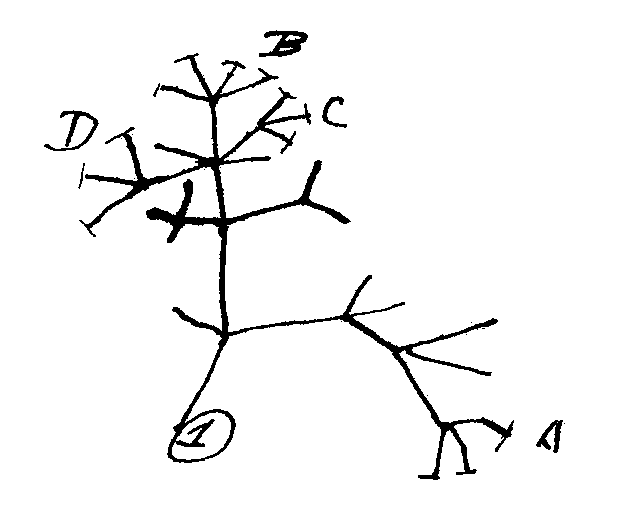
\includegraphics[width=20em]{figures/background2/darwin-tree.png}
  \caption{Charles Darwin's first diagram of an evolutionary tree from his
    notebook \textit{Transmutation of species}, 1837 \cite{darwin1837notebook}.}
  \label{fig:darwin-tree}
\end{figure}

Trees as a formally defined mathematical entity, such as the ones will see in
the following sections, appeared as early as 1847 with the name ``tree''
appearing in the literature shortly afterwards \cite{knuth97taocp1}.  The more
general theory of graphs and topology was developed earlier and is considered
to have begun with Euler who in 1735 presented the paper ``Solutio problematis
ad geometriam situs pertinentis'' \cite{euler1735solutio} in which it was
shown that it was not possible to walk through the city of Königsburg crossing
each of its seven bridges exactly once.

Tree structures are of great importance in computer programming.  One of the
earliest programs to make explicit use of tree structures used them to
represent algebraic formul\ae\ for the purpose of symbolic differentiation
\cite{knuth97taocp1,kahrimanian53differentiation}.  This would later become
the field of computer algebra which would drive the development of computer
science and especially programming languages for many years.

Intuitively, it makes sense to arrange many different types of information in
trees, particularly that for which we can define a distance.  A first question
to ask is whether a representation in terms of a tree exists for a given
dataset and distance function.  As we will see, when the distance function
satisfies certain properties there always exists a tree representation and
this representation is also unique (in a well-defined sense).  We focus then
on a slightly different problem: imagine we know the distance between only
certain pairs of objects in our dataset.  We call this information a partial
distance.  This presents two separate problems.  First, does there exist a
tree representation of a given partial distance and if so, can we find one?
Second, does there exist a unique tree representation of a given partial
distance, and if so can we find it?  These issues are the subject of the
remainder of this thesis.

\subsection{Basic terminology and assumptions}
\label{sec:basic-term-assumpt}

In this section we introduce much of the terminology that is required for
dealing with trees.  Since trees are special cases of graphs, we begin with
general graph theory before moving on to trees and, in particular, a special
type of tree that is of greatest interest to us: the equidistant tree.  As
noted by Knuth \cite{knuth97taocp1} there is a large degree of variation in
the terminology used by different authors in graph theory.  We try to follow
the terminology used in current phylogenetics literature such as
\cite{semple2003phylogenetics} and \cite{dress11lassoing}.  Throughout this
section, let $X$ denote a finite nonempty set.

\subsubsection{Graphs}
\label{sec:graphs}

A \textit{graph} is an ordered pair $(V,E)$ where $V$ is a set of
\textit{vertices} and $E$ is a set (or multiset) of \textit{edges}, each of
the form $\{x,y\}$ such that $x,y \in V$ are distinct.  Unless specified
otherwise, all graphs in this thesis are \textit{simple} and finite meaning
that $V$ and $E$ are finite sets and there are no loops.  Suppose $G = (V,E)$
is a graph. Two vertices $v,v' \in V$ are said to be \textit{adjacent} if
there exists an edge in $G$ joining $v$ and $v'$.  An edge $\{x,y\} \in E$ is
said to be \textit{incident} with the vertices $x$ and $y$.  The
\textit{degree} of a vertex $v \in V$ is the number of edges in $G$ incident
with it.

\begin{figure}
  \centering
  \input{figures/background2/graph-ex.pdft}
  \caption{A graph (i) and a directed graph (ii).}
  \label{fig:graph-ex}
\end{figure}

A \textit{path} is a sequence of distinct vertices $v_1,v_2,\dotsc,v_k$ where
$k \geq 2$ such that for all $i \in \{1,\dotsc,k-1\}, v_i$ and $v_{i+1}$ are
adjacent.  If $k \geq 3$ and $v_1$ and $v_k$ are also adjacent then the path
is called a \textit{cycle}.  A graph is \textit{connected} if between each
pair of distinct vertices there exists a path joining them.  A graph is
\textit{complete} if there is an edge joining each pair of distinct vertices.
A subset $V' \subseteq V$ is called a \textit{clique} if there is an edge
joining each pair of distinct vertices in $V'$.  Figure~\ref{fig:graph-ex}
helps to illustrate these definitions.  In the graph shown in (i) an example
of a path is $g,f,e,d$ and an example of a cycle is $g,f,b,a,g$.  The graph is
connected, but not complete, and the set $\{a,b,g,f\}$ is a clique.

A \textit{directed graph} is an ordered pair $(V,E)$ where $E$ is a set of
\textit{directed edges} or \textit{arcs}.  An arc $(v,v') \in E$ is said to
lead from $v$ to $v'$.  The \textit{out-degree} of a vertex is the number of
arcs leading out from it and the \textit{in-degree} is the number leading in.
The degree of a vertex is therefore the sum of its out-degree and in-degree.
An \textit{oriented path} is a sequence of distinct vertices $v_1,\dotsc,v_k$
such that there exists an arc from $v_i$ to $v_j$ for all $1 \leq i \leq k-1$.
Figure~\ref{fig:graph-ex} (ii) shows a directed graph to help illustrate these
definitions.  Vertex $f$ has out-degree 3, in-degree 1 and therefore degree 4.
An example of an oriented path is $e,f,b,c$.

Two graphs $(V,E)$ and $(V',E')$ are called \textit{isomorphic} if there
exists a bijection $\phi \colon V \to V'$ such that $\{v,v'\} \in E$ if and
only if $\{\phi(v),\phi(v')\} \in E'$.  So, in other words, adjacency of
vertices is preserved.  A graph $(V',E')$ is a \textit{subgraph} of a graph
$(V,E)$ if $V' \subseteq V$ and $E' \subseteq E$.  Further if $V' \subseteq V$
and $E'$ contains all edges $\{v,v'\} \in E$ whenever $v,v' \in V'$ the graph
$(V',E')$ is an \textit{induced subgraph} of $(V,E)$.

\subsubsection{Trees}
\label{sec:trees}

In this section we formally define trees as a special type of graph and
introduce all the relevant terminology for a special type of tree which we
will focus on.

A graph that is connected and has no cycles is called a
\textit{tree}.  Trees can be characterised in many ways, some of which are
given in the following theorem (see \cite[][Section 2.3.4.1]{knuth97taocp1}
for a proof):

\begin{thm}
  If $G$ is a finite graph with $n > 0$ vertices, the following statements are
  equivalent:
  \begin{enumerate}[label=\alph*)]
  \item $G$ is a tree,
  \item $G$ is connected, but if any edge is deleted the resulting graph is no
    longer connected,
  \item There is exactly one path between any two distinct vertices of $G$,
  \item $G$ contains no cycles and has $n-1$ edges,
  \item $G$ is connected and has $n-1$ edges.
  \end{enumerate}
\end{thm}

For example, Figure~\ref{fig:x-tree-ex} shows two graphs which are trees.  The
tree depicted in (ii) is a special type of tree called a \textit{rooted tree}.
A rooted tree (or \textit{oriented tree}) is a directed graph $G$ with a
distinguished vertex $\rho_G$ (the root) such that \cite{knuth97taocp1}:
\begin{enumerate}[label=\alph*)]
\item The root $\rho_G$ has in-degree 0,
\item Each vertex $v$ of $G$ apart from $\rho_G$ has in-degree 1,
\item There is a path between $\rho_G$ and any vertex of $G$ that is not the
  root.
\end{enumerate}

\begin{figure}
  \centering
  \input{figures/background2/x-tree-ex.pdft}
  \caption{A tree (i) and a rooted phylogenetic $X$-tree
    (ii).}
  \label{fig:x-tree-ex}
\end{figure}

Suppose $T$ is a rooted tree.  A vertex in $T$ is called a \textit{leaf} if it
has degree 1.  All other vertices are called \textit{interior} vertices.  An
edge which is incident with a leaf is called a \textit{pendant} edge.  All
other edges are called \textit{interior} edges.  The set of all leaves of $T$
is called the \textit{leafset} of $T$ which we denote by $L(T)$.

Suppose $X$ is a finite, nonempty set, a \textit{rooted phylogenetic $X$-tree}
is a rooted tree with no vertices of in-degree one and out-degree one and with
leafset $X$.  Since the remainder of this thesis is concerned with rooted
trees we will from now on refer to a rooted phylogenetic $X$-tree as simply an
\textit{$X$-tree}.  Figure~\ref{fig:x-tree-ex} (ii) shows an $X$-tree with $X
= \{a,\dotsc,f\}$.

An $X$-tree is \textit{binary} if all interior vertices have degree 3 apart
from the root which has degree 2.  We therefore have that each vertex has
out-degree zero or two and each vertex apart from the root has in-degree 1.
By considering the directed paths from the root to leaves it becomes clear why
such a tree is called binary \cite{semple2003phylogenetics}.

An \textit{edge-weighted graph} $(G,\omega)$ is a graph $G=(V,E)$ paired with
an edge-weighting function $\omega \colon E \to \rr$.  For an edge-weighted
$X$-tree $T$ we call an edge-weighting \textit{proper} if $w(e) > 0$ for every
interior edge $e$ of $T$.

An $X$-tree has a natural partial order on the vertices.  Given an $X$-tree
$T=(V,E)$, a vertex $v \in V$ is an \textit{ancestor} of a vertex $v' \in V$
if and only if $v$ is on the directed path from the root of $T$ to $v'$.  The
vertex $v'$ is then said to be a \textit{descendant} of $v$.  If $v$ and $v'$
are adjacent then we also call $v$ the \textit{parent} of $v'$ and $v'$ a
\textit{child} of $v$.  The number of children of a particular vertex equals
its out-degree.

The \textit{lowest common ancestor} of two vertices $v$ and $v'$ in an
$X$-tree is the unique vertex $u$ such that $u$ is an ancestor of both $v$ and
$v'$ and the path from the root $\rho$ to $u$ is longer than the path to any
other ancestor of both $v$ and $v'$.  The lowest common ancestor of $v$ and
$v'$ is denoted $\lca(v,v')$.  In the $X'$-tree in Figure~\ref{fig:x-tree-ex}
(ii) the lowest common ancestor of $a$ and $d$ is the root $\rho$.

A connected subgraph of a tree is called a \textit{subtree}.  If $T$ is an
$X$-tree and $X' \subseteq X$ then we denote by $T|X'$ the subtree of $T$
whose leafset is $X'$, with degree 2 vertices suppressed.  $T|X'$ is then
called a \textit{restricted subtree}.  If $T$ is binary and $|X'| = 3$ then
$T|X'$ is called a \textit{triplet}.

We call two $X$-trees $T$ and $T'$ \textit{equivalent} (written $T \simeq T'$)
if there exists a bijection $\phi \colon V(T) \to V(T')$ that extends to a
graph isomorphism that is the identity on $X$.  Since an $X$-tree is rooted,
$\phi$ must also map $\rho_{T}$ to $\rho_{T'}$.

For a set $X$ the number of possible non-equivalent binary $X$-trees is
$(2|X|-3)!!$ (where $!!$ means double factorial).  Therefore to find a tree in
this space with particular properties we cannot look at each possible tree and
must instead use a special tree reconstruction method.  Next we look at how
distances are related to trees and then at the problem of reconstructing a
tree from distance information.

\subsubsection{Ultrametrics}
\label{sec:ultrametrics}

Given an edge-weighted $X$-tree $(T,\omega)$ where $T=(V,E)$ and $\omega
\colon E \to \rrnn$ we can associate a distance $D_{(T,\omega)} \colon X
\times X \to \rrnn$ to $(T,\omega)$ by setting for all $x,y \in X$:
\begin{equation*}
  D_{(T,\omega)}(x,y) =
  \begin{cases}
    \displaystyle
    \sum_{e \in P(x,y)} \omega(e) & \text{if $x \neq y$},\\
    0 & \text{otherwise,}
  \end{cases}
\end{equation*}
where $P(x,y)$ is the set of edges on the path from $x$ to $y$.  We call
$D_{(T,\omega)}$ the distance \textit{induced} by $(T,\omega)$.

\begin{figure}
  \centering
    \begin{subfigure}[b]{0.5\textwidth}
      \centering
      \input{figures/background2/treeconstruct1.pdft}
      \label{fig:example-equidistant-1}
      \caption{}
    \end{subfigure}%
    ~
  \begin{subfigure}[b]{0.5\textwidth}
    \centering
    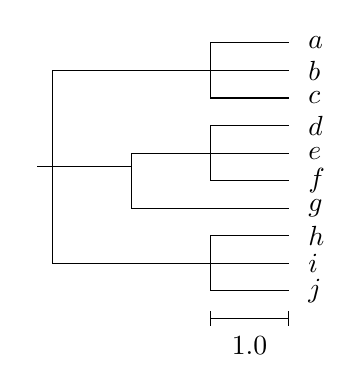
\begin{tikzpicture}[yscale=0.35]
    \node (r) at (0.0,0.0) {};
\node (rr) at (-0.2,0.0) {};
\draw (r.center) -- (rr.center);
\node (r1) at (2.0,-3.5) {};
\node[label=right:{$j$}] (r11) at (3.0,-4.5) {};
\draw (r1.center) |- (r11.center);
\node[label=right:{$i$}] (r12) at (3.0,-3.5) {};
\draw (r1.center) |- (r12.center);
\node[label=right:{$h$}] (r13) at (3.0,-2.5) {};
\draw (r1.center) |- (r13.center);
\draw (r.center) |- (r1.center);
\node (r2) at (1.0,0.0) {};
\node[label=right:{$g$}] (r21) at (3.0,-1.5) {};
\draw (r2.center) |- (r21.center);
\node (r22) at (2.0,0.5) {};
\node[label=right:{$f$}] (r221) at (3.0,-0.5) {};
\draw (r22.center) |- (r221.center);
\node[label=right:{$e$}] (r222) at (3.0,0.5) {};
\draw (r22.center) |- (r222.center);
\node[label=right:{$d$}] (r223) at (3.0,1.5) {};
\draw (r22.center) |- (r223.center);
\draw (r2.center) |- (r22.center);
\draw (r.center) |- (r2.center);
\node (r3) at (2.0,3.5) {};
\node[label=right:{$c$}] (r31) at (3.0,2.5) {};
\draw (r3.center) |- (r31.center);
\node[label=right:{$b$}] (r32) at (3.0,3.5) {};
\draw (r3.center) |- (r32.center);
\node[label=right:{$a$}] (r33) at (3.0,4.5) {};
\draw (r3.center) |- (r33.center);
\draw (r.center) |- (r3.center);
\draw[|-|] (2.0,-5.5) -- (3.0,-5.5);
\node at (2.5,-6.5) {1.0};
     \end{tikzpicture}
     \caption{}
     \label{fig:example-equidistant-2}
   \end{subfigure}

   \caption{A dendrogram is a visual representation of a tree.  Here we see
     two different ways to draw the same edge-weighted $X$-tree.}
   \label{fig:example-equidistant}
\end{figure}

The distance induced by a tree is a special type of metric called a
\textit{tree metric}.  These metrics have some interesting properties which
are discussed in \cite[Chapter 7]{semple2003phylogenetics}.  For our purposes
we are most interested in a special type of tree metric called an
\textit{ultrametric}.  A distance $\delta \colon X \times X \to \rr$ is called
an ultrametric if for every distinct $x,y,z \in X$ the following stronger form
of the triangle inequality holds:
\begin{equation*}
  \delta(x,y) \leq \max(\delta(x,z),\delta(y,z)).
\end{equation*}

An edge-weighting $\omega \colon E \to \rr$ for an $X$-tree $T=(V,E)$ with
root $\rho_T$ is called \textit{equidistant} if it satisfies the following
properties:
\begin{itemize}
\item[(i)] $D_{(T,\omega)}(\rho_T,x) = D_{(T,\omega)}(\rho_T,y)$ for all $x,y
  \in X$,
\item[(ii)] $D_{(T,\omega)}(x,y) \geq D_{(T,\omega)}(x,u)$ for all $x \in X$
  and any $u,v \in V$ whenever $u$ is encountered before $v$ on the directed
  path from $x$ to $\rho$.
\end{itemize}
If $\omega$ is an equidistant edge-weighting then $D_{(T,w)}$ is an
ultrametric \cite[Lemma 7.2.4]{semple2003phylogenetics}.  $X$-trees with
equidistant edge-weightings arise naturally in many places, for example in
phylogenetics.  For convenience we will from now on refer to such an $X$-tree
with equidistant edge-weighting as simply an \textit{equidistant $X$-tree}.

Figure~\ref{fig:example-equidistant} shows an example of an equidistant
$X$-tree with $X = \{a, \dotsc, j\}$ using two common display formats
(dendrograms).  In (i) the edges are simply labelled with their weights (edges
with weight 1 are left unlabelled for clarity).  In (ii) the weight of each
edge is proportional to the horizontal component of its length on the bar with
the actual length shown with a scale bar.

For any ultrametric $\delta \colon X \times X \to \rr$ there is, up to
isomorphism, a unique equidistant $X$-tree $(T,\omega)$ such that $\delta(x,y)
= D_{(T,\omega)}(x,y)$ for all $x,y \in X$.  This tree can be recovered from
the ultrametric in polynomial time, as we will see in the next section.

\section{Tree reconstruction}
\label{sec:tree-construction}

In this section, we look at various methods of reconstructing trees.  Of most
interest to us is the problem of reconstructing an $X$-tree from a distance on
$X$.  This is generally done by one of two broad classes of hierarchical
clustering methods which we discuss in Section~\ref{sec:hier-clust-meth}.

A further problem is that of reconstructing an edge-weighted $X$-tree from a
distance on $X$.  This is desirable in many cases, for example in
phylogenetics the edge-weights might represent the time or number of point
mutations \cite{felsenstein2004inferring}.

Closely related to this is the problem of reconstructing $X$-trees from only
partial distance information.  This means that we do not have the complete
distance $d$, but rather only have the values $d(x,y)$ for some, but not all,
pairs $x,y \in X$.  This problem is motivated by the fact that accurate
distance measurements are often difficult or impossible to obtain in practice
but one would still like to build an edge-weighted $X$-tree given only what is
known.

As with complete distance information, it is possible for partial distance
information to uniquely determine an $X$-tree.  This is the subject of
Section~\ref{sec:lassoing-corralling}.  This allows us to define a consistency
property for partial distance reconstruction methods.

\subsection{Reconstruction from subtrees}
\label{sec:constr-from-subtr}

Before we look at reconstructing trees from distances, it is interesting to
note that we do not actually need a distance to reconstruct only the topology
of an $X$-tree.  It suffices merely to know the set of subtrees displayed by
the tree \cite{semple2003phylogenetics}.

A pair of leaves of an $X$-tree that share the same parent is called a
\textit{cherry} and a set of leaves (of any size) that share the same parent
is called a \textit{pseudocherry}.  As before, an $X$-tree with $|X| = 3$ that
contains a cherry is called a triplet.  If $P$ is an $\{a,b,c\}$-tree $a,b$ is
a cherry of $P$ then we denote the triplet $P$ by $ab|c$.  We say that a
triplet $ab|c$ is \textit{displayed} by an $X$-tree $T$ if the restriction
$T|\{a,b,c\}$ of $T$ to $\{a,b,c\}$ is binary and $lca_T(a,c) = lca_T(b,c)$ is
an ancestor of $lca_T(a,b)$ in $T$.  For example, the tree $T_2$ in
Figure~\ref{fig:build-ex} is a triplet and can be written as $ad|c$.

\begin{figure}
  \centering
  \input{figures/background2/build-ex2.pdft}
  \caption{An illustration of \textsc{Build} with an input of $R =
    \{T_1,T_2\}$.  $[R,S]$ is the auxiliary graph built in the first iteration
    of the algorithm and $T$ is the final tree constructed.}
  \label{fig:build-ex}
\end{figure}

The \textsc{Build} algorithm \cite{aho1981inferring} can be used to
reconstruct an $X$-tree $T$ from the set of all triplets displayed by $T$.  We
show the \textsc{Build} algorithm in pseudocode in Algorithm~\ref{alg:build}
and give an example in Figure~\ref{fig:build-ex}.  The algorithm uses a set
$R$ of rooted trees $\{T_1,\dotsc,T_n\}$ where $L(T_1) \cup \dotsb \cup L(T_n)
= X$ and an auxiliary graph $[R,S]$ which has vertex set $S \subseteq X$ and
an edge $\{a,b\}$ for each $a,b \in S$ whenever there exists some $c \in S$
and some $T' \in R$ such that $T'|\{a,b,c\}$ and $ab|c$ are equivalent.

\begin{algorithm}
  \caption{\textsc{Build}.}
  \label{alg:build}

  \begin{algorithmic}
    \Require A set of rooted trees $R = \{T_1,\dotsc,T_n\}$.
    \Ensure  An $X$-tree $T$ where $X = L(T_1) \cup \dotsb \cup L(T_n)$.

    \State $S = \{x_1,\dotsc,x_m\} \gets X$.

    \If{$|S| = 1$} \Return the tree $(\{x_1\},\emptyset)$. \EndIf

    \If{$|S| = 2$} let $\rho$ be a new vertex and \Return the tree with root
    node $\rho$ obtained by attaching $x_1$ and $x_2$ to $\rho$. \EndIf

    \State Construct the auxiliary graph $[R,S]$.

    \State Let $S_1,\dotsc,S_k$ be the vertex sets of the connected components
    of $[R,S]$.

    \ForAll{$1 \leq i \leq k$}
    \State Let $T_i$ be the output of \textsc{Build} on $R_i =
    \{T|S_i \colon T \in R\}$.
    \EndFor

    \State Let $\rho$ be a new vertex and \Return the tree with root node
    $\rho$ obtained by attaching the root of each $T_i$ to $\rho$.
    
  \end{algorithmic}
\end{algorithm}

This algorithm has some nice properties, for example if \textsc{Build} returns
a tree then the set of input trees is said to be \textit{compatible}.  The
definition of compatible is independent of \textsc{Build} (see
\cite{semple2003phylogenetics}) but \textsc{Build} can be used to check
compatibility.  Furthermore, if we input the set of all triplets displayed by
a tree $T$, then \textsc{Build} is guaranteed to output $T$ and therefore $T$
is uniquely determined by the set of triplets it displays.

If the inputted set of triplets $R$ is some subset of all the triplets
displayed by a tree then the set is still compatible but this set is displayed
by possibly many trees.  In this case the output of \textsc{Build} is
deterministic and the tree reconstructed is known as \textit{the
  \textsc{Build} tree for $R$}.  Some interesting properties of these trees
can be found in \cite[Section 2.5.2]{bryant97buildingtrees}.

The \textsc{Build} algorithm was initially developed to construct a tree
satisfying a given set of constraints and was applied to problems arising in
the theory of relational databases.  It was later applied to phylogenetics but
remained relatively unknown in the field for a number of years
\cite{steel1992complexity,bryant04supertree}.

When the inputted trees are not compatible, \textsc{Build} returns an error.
Since it is often the case that trees will not be compatible, the
\textsc{MinCutSupertree} algorithm was developed which will construct a tree
even if the input trees are not compatible \cite{semple2000supertree}.
The algorithm builds a graph similar to $[R,S]$ and ensures that it is
disconnected in each step by using a minimum cut.  This algorithm was
developed primarily for construction of phylogenetic supertrees.

\subsection{Reconstruction from distances}
\label{sec:constr-from-dist}

We now turn to the problem of reconstructing an $X$-tree from a distance.  We
begin with a brief overview of general hierarchical clustering methods and
then look at the UPGMA method \cite{sokal1958statistical} and its optimal
runtime algorithm.  Hierarchical clustering methods in general build
unweighted $X$-trees, but UPGMA can be considered an extension which also
constructs an edge-weighting for the constructed tree.

For a distance-based reconstruction method the following property is
desirable: if we input a distance function $D_{(T,\omega)}$ induced by an
edge-weighted $X$-tree $(T,\omega)$ we get the tree $T$ and its edge-weighting
$\omega$.  If a method enjoys this property then we call it
\textit{consistent}.  For many methods this property holds only under certain
conditions.  For UPGMA this holds if $(T,\omega)$ is a binary equidistant
$X$-tree \cite{durbin1998biological}.

\subsubsection{Hierarchical clustering methods}
\label{sec:hier-clust-meth}

\begin{figure}
  \centering
  \input{figures/background2/tree-clust-ex.pdft}
  \caption{A tree can be viewed as a hierarchy of partitions.}
  \label{fig:tree-clust-ex}
\end{figure}

Hierarchical clustering is used for the classification of information in much
the same way as partitional clustering.  The aim of a hierarchical clustering
method is to produce an $X$-tree corresponding to a given distance $D$ on a
set $X$.  While a partition of a set is merely a set of disjoint subsets
(clusters) which ``cover'' the set, an $X$-tree can be viewed as a hierarchy
of such clusters which induces several partitions on $X$.  This natural
relationship between trees and partitions is illustrated in
Figure~\ref{fig:tree-clust-ex}.  In the example we have $X = \{a,\dotsc,e\}$.
The root of the tree corresponds to the single cluster $X$ (denoted $abcde$)
and as we move down the tree the set is partitioned further until we have
cluster of one leaf each ($\{\{a\},\dotsc,\{e\}\}$, denoted $a|b|c|d|e$ for
short).

There are two main methods in use for building hierarchies.  These are the
\textit{agglomerative} or ``bottom-up'' methods which begin with each element
of $X$ in its own cluster and successively merges clusters until there is only
one cluster left, and the \textit{divisive} or ``top-down'' methods which
begin with a single cluster and successively splits clusters until each
element is on its own.  The resulting hierarchy depends upon which merges or
splits have been chosen at each stage which, in turn, depends on finding a
local optimum according to some criterion.

\begin{algorithm}[h]
  \caption{Agglomerative hierarchical clustering algorithm.}
  \label{alg:agglomerative}

  \begin{algorithmic}
    \Require A set $X$ and a linkage function $D \colon 2^X \times 2^X \to \rr$
    with an underlying distance $d \colon X \times X \to \rr$.

    \Ensure  A rooted $X$-tree $T$.

    \State Let $F$ be a forest of $|X|$ trees each containing a unique element
    of $X$ as the only vertex, which is also the root,

    \While{$|F| > 1$}

       \State Let $v$ be a new vertex and $\displaystyle (x,y) \gets \argmin_{x,y
         \in F} D(L(x),L(y))$,
       \State Remove trees $x$ and $y$ from $F$ and add the tree obtained by
         attaching the roots of $x$ and $y$ to $v$ and letting $v$ be the root,
    
    \EndWhile

    \State \Return the single tree contained in $F$.
    
  \end{algorithmic}
\end{algorithm}

The general algorithm for agglomerative clustering is shown in
Algorithm~\ref{alg:agglomerative}.  The choice of linkage function determines
how the distances are recomputed at each stage and therefore which trees are
joined in each subsequent stage.  Given a set $X$ and distance $d \colon X
\times X \to \rr$ and two nonempty subsets $C_1,C_2 \subseteq X$, some common
choices for linkage functions include:\\
single-linkage:
\begin{equation*}
  \label{eq:slink}
  D_{SL}(C_1,C_2) = \min_{x \in C_1, y \in C_2} d(x,y),
\end{equation*}
complete-linkage:
\begin{equation*}
  \label{eq:clink}
  D_{CL}(C_1,C_2) = \max_{x \in C_1, y \in C_2} d(x,y),
\end{equation*}
and average-linkage:
\begin{equation*}
  \label{eq:alink}
  D_{AL}(C_1,C_2) = \left(\,\sum_{x \in C_1} \sum_{y \in C_2} d(x,y) \right) / |C_1| |C_2|.
\end{equation*}

The general algorithm for agglomerative clustering has runtime complexity of
$O(n^3)$ where $n = |X|$ since there are $O(n)$ merges to be done and finding
the $\argmin$ takes $O(n^2)$ time.  However, for many linkage criteria,
including the three above, it is possible to use an $O(n^2)$ algorithm.  Two
well known examples are SLINK \cite{sibson1973slink} and CLINK
\cite{defays1977efficient} for using single-linkage and complete-linkage
respectively.  In the next section we will see that hierarchical clustering
using average-linkage may be done in quadratic time too.

The divisive method works in the opposite direction: we begin with a single
cluster and successively split clusters until we end up with one cluster per
leaf.  Divisive methods are usually significantly more complicated than
agglomerative methods.  Each step requires an initial decision about which
cluster to split, and then a decision about how to split that cluster
\cite{savaresi2002cluster}.  A naïve approach for deciding which cluster to
split next is to always split the largest cluster, but there are more
sophisticated approaches, for example based on cluster homogeneity.  Splitting
a cluster then essentially requires a partitional clustering method
\cite{ding2002cluster}.  In general the time complexity of a divisive method
is $O(2^n)$ where $n = |X|$ making it prohibitively expensive for most
applications \cite{cimiano2004comparing}.

\subsubsection{UPGMA}
\label{sec:upgma}

Unweighted Pair Group Method with Arithmetic Mean (UPGMA)
\cite{sokal1958statistical} is in fact a modified agglomerative clustering
method using average-linkage which reconstructs an equidistant $X$-tree.  For
an equidistant $X$-tree $(T,\omega)$, let $height((T,\omega))$ be the sum of
the edge weights on the path from the root of $T$ to any leaf, or 0 if the
root is the sole vertex.  The algorithm for UPGMA is shown in
Algorithm~\ref{alg:upgma}.

\begin{algorithm}[h]
  \caption{UPGMA.}
  \label{alg:upgma}

  \begin{algorithmic}
    \Require A set $X$, and a distance $d \colon X \times X \to \rr$.
    \Ensure  A binary equidistant $X$-tree $(T, \omega)$.

    \State Let $F$ be a forest of $|X|$ trees each containing a unique element
    of $X$ as the only vertex, which is also the root.

    \While{$|F| > 1$}

       \State Let $v$ be a new vertex,
       \State put $\displaystyle m \gets \min_{x,y \in F} D_{AL}(L(x),L(y))$,
       \State and $\displaystyle (x,y) \gets \argmin_{x,y \in F} D_{AL}(L(x),L(y))$.
       \State Remove trees $x$ and $y$ from $F$ and add the tree obtained by
         attaching the root of $x$ to $v$ with an edge of length $m/2 -
         height(x)$, attaching the root of $y$ to $v$ with an edge of length
         $m/2 - height(y)$ and letting $v$ be the root.
    
    \EndWhile

    \State \Return the $X$-tree contained in $F$ and its edge-weighting.
  \end{algorithmic}
\end{algorithm}

Since only two trees are joined in each iteration, the output of UPGMA is
always a binary tree.  If the input distance $d$ is equal to the induced
distance $D_{(T,\omega)}$ of some equidistant binary $X$-tree $(T,\omega)$
then UPGMA is guaranteed to return $(T,\omega)$ \cite{durbin1998biological}.

% mention general method for other linkage criteria

% However, for all three of the linkage
% functions above there are special algorithms which run in only $O(n^2)$ time,
% these are SLINK \cite{sibson1973slink}, CLINK \cite{defays1977efficient} and
% UPGMA respectively.  The following section discusses .

In the general agglomerative algorithm, each step involves identifying a pair
of elements such that no other pair of elements in $X$ are closer according to
the chosen linkage criterion.  In other words, we are finding a global
minimum.  In more efficient algorithms we instead look only for a local
minimum at each stage.  A local minimum in this context means a pair of
elements which are \textit{mutual nearest neighbours} (MNNs).  Given a set $X$
and a distance $d$ on $X$, a pair $x,y \in X$ are MNNs if there exists no
element $z \in X$ for which $d(x,z) < d(x,y)$ or $d(y,z) < d(x,y)$.  Such a
pair can be safely agglomerated as soon as it is found, just as in the general
algorithm \cite{murtagh2011methods}.

Finding MNNs can be done quickly by building a chain of nearest neighbours in
the following way: we begin with an arbitrary cluster in $X$ and find its
nearest neighbour giving us a chain of length two.  We then repeatedly add to
the chain the nearest neighbour of the last element in the chain until we find
a pair of MNNs.  The MNNs are removed from the chain and agglomerated.  The
distances between new clusters and all other clusters are calculated
recursively using the Lance-Williams update formula in constant time
\cite{lance66theory}.  The process is then continued from the end of the
chain, or from an arbitrary cluster if the chain is empty.  This method works
because for certain linkage criteria, including average-linkage, the nearest
neighbour chain remains valid after an agglomeration (see
\cite{gronau2007optimal} for details).

This mutual nearest neighbour method, also called the \textit{algorithme des
  célibataires}, was developed in the early 1980s and initially appeared in
\cite{de1980classification} and \cite{juan1982programme} (in French) and later
in \cite{murtagh1983survey} and \cite{murtagh1984complexities} (in English).
It leads to the optimal $O(n^2)$ version of UPGMA and other hierarchical
clustering methods \cite{gronau2007optimal}.

\subsection{Reconstruction from partial distances}
\label{sec:constr-from-part}

Partial distances arise often in practice, that is a distance where the
distance between some pairs of elements is missing.  Potential reasons for
this might be that it is sometimes difficult or impossible to make
measurements between certain pairs due to those pairs not sharing any
information from which a distance can be inferred.  For example, in biological
studies involving large numbers of species and genes it is often the case that
species do not share any genes in the available data
\cite{criscuolo2008fastnj}.  We discuss the motivation for studying this
problem in more detail in Section~\ref{sec:lasso-motivation}.

For this reason it becomes useful to ask whether a partial distance can be
extended into a complete distance that is also an ultrametric.  More formally,
a \textit{partial distance} on $X$ is a function $d^* \colon (X \times X) - M
\to \rrnn$ where $M$ is the set of pairs for which the distance value is
missing.  The problem is to find a complete distance $d \colon X \times X \to
\rrnn$ where $d(x,y) = d^*(x,y)$ for all $x,y \in (X \times X) - M$ and which
is an ultrametric.  In \cite{farach1995robust} it was shown that it is
possible to decide in polynomial time whether an extension to an ultrametric
exists (and to compute such an extension), although the corresponding decision
problem for unrooted trees (that is, deciding if an extension to a general
tree metric exists) is NP-complete.

Below we describe three different methods proposed in the literature for
extending a partial distance on $X$ to an ultrametric on $X$ and
reconstructing the corresponding equidistant $X$-tree.  We restrict ourselves
to equidistant $X$-trees but similar results on unrooted trees may be found
in, for example, \cite{guenoche1999approximations}, \cite{farach1995robust},
\cite{makarenkov2001nouvelle} and \cite{guenoche2004extension}.

\subsubsection{An optimisation method}
\label{sec:part-dist-optim-method}

The approach taken by \citet{de1984ultrametric} is to consider a least squares
constrained optimisation problem.  Given a partial distance $d^* \colon (X
\times X) - M \to \rrnn$, a function $Loss \colon \rrnn^{X \times X} \to
\rrnn$ (where $\rrnn^{X \times X}$ is the set of all dissimilarities on $X$)
is defined as:
\begin{equation*}
  \label{eq:partial-dist-least-squares}
  Loss(d) = \sum_{(x,y) \in (X \times X) - M} \!\big(d^*(x,y)-d(x,y)\big)^2.
\end{equation*}
This is called the \textit{loss function}.  The problem is now to find a
function $d \colon X \times X \to \rrnn$ such that $Loss(d)$ is minimised and
with the constraint that $d$ is an ultrametric.

To solve the constrained minimisation problem the authors propose to use the
sequential unconstrained minimisation technique (SUMT)
\cite{fiacco1964sequential}.  Under this technique the constraint that $d$ be
an ultrametric is removed and instead we find a distance $d_n \colon X \times
X \to \rrnn$ which minimises the augmented function $\Phi \colon \rrnn^{X
  \times X} \times \rrnn \to \rrnn$ defined as:
\begin{equation*}
  \label{eq:partial-dist-optimisation}
  \Phi(d_n,\sigma) = Loss(d_n) + \sigma Pen(d_n), \qquad (\sigma > 0),
\end{equation*}
where $Loss$ is the loss function and $Pen \colon \rrnn^{X \times X} \to
\rrnn$ is called the \textit{penalty function} which is meant to enforce the
ultrametric condition.  $Pen$ is defined as:
\begin{equation*}
  \label{eq:penalty-function}
  Pen(d_n) = \sum_{(i,j,k) \in \Omega(d_n)} \! \big(d_n(i,k) - d_n(j,k)\big)^2
\end{equation*}
where
\begin{equation*}
  \Omega(d_n) = \{(i,j,k) \in X^3 \colon d(i,j) \leq \min\big(d_n(i,k),d_n(j,k)\big)
  \text{ and } d_n(i,k) \neq d_n(j,k)\}.
\end{equation*}
In other words, $\Omega(d_n)$ denotes the set of $3$-tuples for which the
ultrametric condition is violated.  The unconstrained minimisation is
performed successively with an increasing value for $\sigma$, each time using
the previous result $d_{n-1}$ to begin the search for the next $d_n$.  A
method by \cite{powell1977restart} is used to perform the unconstrained
minimisation.

\subsubsection{An agglomerative method}
\label{sec:part-dist-agglom-method}

Missing Values Linkage (MVL) is an example of an agglomerative approach
proposed by \cite{schader1992mvl}.  It is actually identical to the
agglomerative hierarchical clustering algorithm (see
Section~\ref{sec:hier-clust-meth}) but using a linkage criterion modified to
take into account missing values.

The modified
average-linkage criterion for two nonempty sets $S_1, S_2$ is:
\begin{equation*}
  D_{MVL}(S_1,S_2) =
  \begin{cases}
    \displaystyle
    \frac{\displaystyle \sum_{(x,y) \in (S_1 \times S_2) - M} d(x,y)}
         {|(S_1 \times S_2) - M|} & \text{if $(S_1
      \times S_2) - M \neq \emptyset$,} \\
    \infty & \text{otherwise},
  \end{cases}
\end{equation*}
where $M = \{(i,j) \in X \times X \colon d(i,j) \text{ is unknown}\}$.
Modified versions of other linkage criteria are possible; some more examples
are given in the original paper.

The authors do not provide an algorithm with better time complexity than that
of the naïve $O(n^3)$ agglomerative algorithm (where $n = |X|$).  They also
show that the MVL method produces very similar results to
\citeauthor{de1984ultrametric}'s method.

Figure~\ref{fig:farach-mvl-ex} (ii) shows the tree constructed by MVL from a
partial distance $d$ on a set $\{a,\dotsc,e\}$ containing only the distances
$d(a,b)=1, d(b,c)=1, d(c,d)=2, d(c,e)=2, d(d,e)=3$.

\subsubsection{A divisive method}
\label{sec:part-dist-divisive-method}

\citet{farach1995robust} use a top down, divisive approach.  Given a partial
distance function $d^* \colon (X \times X) - M \to \rrnn$ let $G=(V,E)$ be a
graph with vertex set $X$ and an edge $\{x,y\}$ with $x,y \in X$ but $(x,y)
\notin M$ (so the distance between $x$ and $y$ is known).  We also define an
edge-weighting $\omega \colon E \to \rr$ by $\omega(\{x,y\}) = d^*(x,y)$ for
all $x,y \in E$.

The tree reconstruction algorithm proceeds as follows:
\begin{enumerate}
\item If $E = \emptyset$, return the single element in $V$.
\item Otherwise, put $m \gets max_{e \in E} \omega(e)$.
\item Let $G^* = (V,E^*)$ be a graph and put $E^* \gets \{e \in E \colon
  \omega(e) < m\}$.
\item Let $u$ be a new vertex and return the tree with root node $u$ obtained
  by recursing on each connected component of $G^*$ and attaching the results
  of each to $u$.               %what if only one component?!
\end{enumerate}
This basic algorithm shown here requires $O(|V||E|)$ time but a quicker
algorithm requiring only $O(|E| + |V|\log |V|)$ time is also given by
\cite{farach1995robust}.

Figure~\ref{fig:farach-mvl-ex} (i) shows the tree constructed by this method
from the same partial distance $d$ on $\{a,\dotsc,e\}$ containing only the
distances $d(a,b)=1, d(b,c)=1, d(c,d)=2, d(c,e)=2, d(d,e)=3$.  Note that the
tree constructed is different to the tree constructed by MVL.

\begin{figure}
  \centering
  \input{figures/background2/farach-mvl-ex.pdft}
  \caption{The two different trees constructed by Farach's method (i) and the
    MVL method (ii) from the same partial distance information.}
  \label{fig:farach-mvl-ex}
\end{figure}

\section{Lassos}
\label{sec:lassoing-corralling}

As we saw in the example shown in Figure~\ref{fig:farach-mvl-ex}, the existing
partial distance reconstruction methods can construct different trees from the
same input.  The problem with the example partial distance in that case was
that no ultrametric extension exists so the methods each modified the given
distances in different ways to obtain an ultrametric.  This means that for
some pairs of leaves in the resulting tree the induced tree distance is not
equal to the inputted distance.  This may be undesirable.

A second problem is that often more than one extension to an ultrametric is
possible.  We will see this in the example in the following section.  In the
case where more than one extension is possible the existing algorithms will
provide one of many solutions.  But we may wish to know not only that an
ultrametric extension exists but that it is unique.  This section provides us
with some theory for deciding when this is possible.

Certain partial distances on $X$ have the property that they uniquely
determine the topology or edge-weights of an $X$-tree.  In other words, only
one extension to an ultrametric on $X$ is possible.  To enable us to
understand when partial distances have this uniqueness property, the theory of
lassos was developed.  We next define certain types of lassos as applied to
equidistant $X$-trees and look at some important characterisations.

\subsection{Definitions and basic properties}
\label{sec:defin-basic-prop}

Let $(T,\omega)$ and $(T',\omega')$ be two edge-weighted $X$-trees and $\cL
\subseteq {X \choose 2}$ be some subset of pairs of elements in $X$.  For
convenience we denote an element $\{x,y\} \in \cL$ as simply $xy$.  Then
$(T,\omega)$ and $(T',\omega')$ are called \textit{$\cL$-isometric} if
$D_{(T,\omega)}(x,y) = D_{(T',\omega')}(x,y)$ for all $xy \in \cL$.

Now, given an $X$-tree $T$ and a subset $\cL \subseteq {X \choose 2}$ we
define $\cL$ to be:
\begin{enumerate}[label=(\roman*)]
\item an \textit{equidistant lasso} for $T$ if $\omega = \omega'$ holds for
  all equidistant edge-weightings $\omega,\omega'$ of $T$ where $(T,\omega)$
  and $(T,\omega')$ are $\cL$-isometric,
\item a \textit{topological lasso} for $T$ if $T$ is equivalent to $T'$ for
  any $X$-tree $T'$ for which there exist proper edge-weightings $\omega$ and
  $\omega'$ of $T$ and $T'$ respectively where $(T,\omega)$ and $(T',\omega')$
  are $\cL$-isometric,
\item a \textit{strong lasso} $T$ if $\cL$ is both an equidistant and
  topological lasso for $T$.
\end{enumerate}

\begin{figure}
\begin{center}
\input{figures/background2/lasso-example.pdft}
\end{center}
\caption{Two equidistant $X$-trees.  All edges have weight 1 except bold edges
  which have weight 2.  For $\cL=\{ac,de,bc,ce,cd\}$ both trees induce the
  same distances over the cords in $\cL$ despite having different topologies.
  In this case $\cL$ is not a topological lasso.}
\label{fig:lasso-example}
\end{figure}

To illustrate these concepts consider the two equidistant $X$-trees
$(T,\omega)$ and $(T',\omega')$ depicted in Figure~\ref{fig:lasso-example}.
The edge-weights on the edges are proportional to the length of the edges as
shown and induce distances $D_{(T,\omega)} \colon X \times X \to \rr$ and
$D_{(T',\omega')} \colon X \times X \to \rr$ respectively.  The trees are
therefore equidistant.  If we have the set of cords $\cL=\{ac,de,bc,ce,cd\}$
then notice that the distances between each of these pairs of leaves is the
same according to the induced distances for both trees (for example
$D_{(T,\omega)}(a,c) = D_{(T',\omega')}(a,c)$).  Therefore $\cL$ is not a
topological lasso.  Notice that this property of $\cL$ is dependent solely on
the structure of the set itself and not on the actual distances on the trees.
For further information and discussion about lassos, especially those
concerning more general trees, the reader is referred to
\cite{dress11lassoing} and \cite{huber2014tree}.

\subsection{Characterising lassos: the child-edge graph}
\label{sec:lassoing-rooted-x}

Lassos for $X$-trees can be characterised using a graph associated to each
interior vertex of a tree \cite{huber13lassoing}.  First, a lasso $\cL$ of $X$
which satisfies the property that $\bigcup_{c \in \cL} c = X$ is called a
\textit{covering} of $X$.  Let $T$ be an $X$-tree and $\iV(T)$ denote the set
of internal vertices of $T$.  For some $v \in \iV(T)$, and a set of cords $\cL
\subseteq {X \choose 2}$, we associate a graph called $G(\cL,v)$ defined as
follows.  The vertex set of the graph $V_v$ is the set of all child edges of
$v$.  The edge set $E_v$ is the set of all $\{e,e'\} \in {V_v \choose 2}$ for
which there exist leaves $a,b \in X$ and a cord $ab \in \cL$ such that $e$ and
$e'$ are edges on the path from $a$ to $b$ in $T$.  We call the graph
$G(\cL,v)$ the \textit{child-edge graph} (\textit{of $v$ with respect to $T$
  and $\cL$}).

We have the following characterisation of topological lassos which originally
appeared in \cite{huber13lassoing}:
\begin{thm}
  \label{thm:child-edge-graph-complete}
  Suppose $T$ is an $X$-tree and $\cL \subseteq {X \choose 2}$ is a covering
  of $X$.  Then the following are equivalent:
  \begin{enumerate}
  \item $\cL$ is a topological lasso for $T$,
  \item for every vertex $v \in \iV(T)$, the graph $G(\cL,v)$ is complete.
  \end{enumerate}
\end{thm}

Due to the characterisation of equidistant lassos also presented in
\cite{huber13lassoing}, we also have that every topological lasso for $T$ must also be an
edge-weight lasso, and therefore a strong lasso, for $T$.

%%% Local Variables:
%%% TeX-master: "thesis"
%%% End:


% \chapter{Constructing Supertrees from Partial Distances}
\label{cha:constr-ultr-supertr}

\section{Summary}
\label{sec:con-summary}

It is well-known that an edge-weighted tree can be constructed from the matrix
if graph-theoretic distances between its leaf nodes.  This chapter considers
the problem of constructing trees from only partial distances.

\section{Lassoing binary ultrametric trees}
\label{sec:lass-ultr-trees}

An algorithm has been developed that constructs a binary ultrametric tree from
a given lasso.  The algorithm is based on the \textsc{BUILD} algorithm.



%%% Local Variables:
%%% TeX-master: "thesis"
%%% End:


\chapter{Contributions}
\label{cha:contributions}

This chapter contains a brief outline of the original contributions made by
the candidate to date.
\begin{itemize}
\item Showed that minimisation of the centroid-distance ($k$-means)
  homogeneity criterion is not equivalent to maximisation of the separation
  criterion when a mixed-data metric is used.  This means that the commonly
  used centroid-distance criterion should not generally be considered a
  criterion for the separation of clusters,
\item Proved that the \textsc{All-Squares Clustering} problem is NP-complete
  with a 3-valued metric by transformation from the \textsc{Partition into
    Triangles} problem, then proved that it is NP-complete with a $p$-valued
  metric whenever $p\geq 3$,
\item Proved that the \textsc{Centroid-Distance Clustering} problem is
  NP-complete with a 3-valued metric by transformation from the
  \textsc{Dominating Set} problem, then proved that it is NP-complete with a
  $p$-valued metric whenever $p\geq 3$,
\item Developed the Assignment Metric for comparing nonempty subsets of a
  metric space of arbitrary size.  The assignment metric can be used to
  compare partitions while taking into account the underlying metric space of
  the data, which is a major improvement on current methods for comparison of
  partitions,
\item Implemented the Assignment Metric for testing and comparison with other
  existing metrics,
\item Proved that a particular type of cover for a tree is a strong lasso,
\item Developed an algorithm for constructing a tree from a strong lasso,
  similar to the \textsc{Build} algorithm,
\item Implemented a simple framework for working with trees and the strong
  lasso construction algorithm for testing purposes.
\end{itemize}

%%% Local Variables:
%%% TeX-master: "thesis"
%%% End:


\chapter{Further Work}
\label{cha:further-work}



%%% Local Variables:
%%% TeX-master: "thesis"
%%% End:


\bibliographystyle{plainnat}
\bibliography{metrics.bib,comp-clustering.bib,clustering.bib,phylogenetics.bib}

\end{document}
